% =============================================================================
%  VERSION ENSAE  --  rapport de stage de fin d'etudes, Mastere specialise (MS)
%  Actuariat, annee scolaire 2025-2026.
%
%  DEPUIS LE 1er OCTOBRE 2026, CETTE VERSION ET LA VERSION INSTITUT SONT DEUX
%  DOCUMENTS. main_institut.tex est la version complete et figee : il n'est plus
%  genere depuis ce fichier, et refaire_tout.py verifie qu'il garde le contenu de
%  son PDF committe. Seule la version ENSAE se reduit, sous 100 pages, pour suivre
%  les consignes MS du service des stages (demande de Caroline Hillairet).
%
%  LA REDUCTION SUIT LA MISSION ECRITE EN TETE DU CLAUDE.md A LA RACINE (branche
%  reduction-sfe). Elle ne modifie que la version ENSAE : les fichiers qu'elle cree ou
%  change ne doivent jamais etre lus par main_institut.tex, qui reste tel quel.
%
%  ETAT : PHASE 3 DE LA REDUCTION, restructuration a texte constant. Cette version lit
%  ses chapitres dans chapitres_sfe/, copies de chapitres/ reorganisees selon le plan
%  cible de la mission : introduction, dix chapitres, conclusion, enseignements du
%  stage, bibliographie, annexes A a D, puis les deux notes de synthese en fin de
%  fichier (ordre impose par les consignes MS). Correspondance des sections :
%  reduction/phase3_correspondance.md. Le contenu retire (anciennes annexes B et F,
%  questionnaire d'elicitation) est dans supplement/, et les renvois du corps vers lui
%  passent par les etiquettes relais de la notice des annexes. Couverture :
%  garde_ensae.tex (phase 2). Etat de depart : etiquette avant-reduction.
%
%  FICHIER A DEPOSER : KADDOURI_Kelian_MS25.pdf (NOM_Prenom_MS25.pdf, consignes
%  MS 2025-2026), ou le meme suffixe _CONF si le rapport devenait confidentiel.
%  Depot sur la plateforme des stages AVANT LE 14 OCTOBRE 2026 A 17 H, date
%  previsionnelle, delai de rigueur.
% =============================================================================

\documentclass[12pt,a4paper]{report}

% FORMAT IMPOSE PAR L'ECOLE : Times New Roman 12 et interligne 1,5. La commande ci-dessous
% active, dans le preambule partage, la branche Times et 1,5 ; les autres versions ne la
% definissent pas et gardent Palatino 11. L'ecole a leve la limite de trente pages le
% 16 septembre 2026, pas la police ni l'interligne.
\newcommand{\formatensae}{}

% Meme preambule que la version 2, qui est la reference de style du projet.
% Préambule V2 : STYLE CLASSIQUE DE MONOGRAPHIE. Appelé par main_v2.tex.
%
% CE FICHIER NE CHANGE QUE L'APPARENCE. Les chapitres sont EXACTEMENT les mêmes
% fichiers que ceux de main.tex : aucun mot, aucun nombre, aucune structure ne
% diffère entre les deux versions. C'est la condition pour que la comparaison
% porte sur le style seul, et c'est aussi ce qui évite de maintenir deux textes.
%
% CE QUI CHANGE, ET POURQUOI
%   1. POLICE. Palatino (mathpazo) au lieu de Latin Modern. C'est une romaine de
%      la Renaissance revisitée : c'est elle qui donne l'aspect << texte ancien >>.
%      Sa hauteur d'x est grande, donc l'interligne est ouvert à 1,05, sans quoi
%      le gris de la page devient trop dense.
%   2. AUCUNE COULEUR. Tous les noms de couleurs du projet sont redéfinis en NOIR,
%      ce qui neutralise les \textcolor{navy} des chapitres sans les éditer. Les
%      liens restent cliquables mais s'impriment en noir.
%   3. LES ENCADRÉS DEVIENNENT DES FILETS. Les 66 blocs << clé >> et les 48 blocs
%      << attention >> perdent leur fond bleu et leur cadre arrondi. Ils gardent
%      leur distinction, mais par la TYPOGRAPHIE et non par la couleur : filets
%      haut et bas pour la synthèse, filet vertical épais pour l'avertissement.
%      C'est le dispositif des monographies imprimées, et il survit à la
%      photocopie comme à l'impression en noir et blanc.
%   4. TITRES. Petites capitales et filets, jamais de gras coloré. Les têtes de
%      paragraphe passent en italique : elles sont ici des phrases entières, et
%      une phrase entière en gras alourdit la page.
%   5. TITRES COURANTS. Chapitre en petites capitales en tête de page. Signal
%      classique, et utile sur un document de cette longueur.
%
% CE QUI NE CHANGE PAS, ET C'EST DÉLIBÉRÉ
%   LA GÉOMÉTRIE. Les marges restent à 2,4 cm. Une monographie classique aurait
%   une justification plus étroite, mais la lisibilité des cinquante figures est
%   calibrée sur CETTE largeur : \figover déborde à 1,14 fois la justification et
%   \figcle remplit la page. Rétrécir le bloc de texte rendrait les étiquettes
%   illisibles, ce qui est le défaut que la note de \figover documente. Le style
%   ne se paie pas en lisibilité des résultats.
%
%   LES CHIFFRES RESTENT ALIGNÉS (pas de chiffres elzéviriens). Palatino en
%   propose, et ils sont plus élégants dans un texte courant. Ils sont refusés
%   ici : ce document se lit pour ses nombres, et des chiffres de hauteur
%   inégale se comparent mal dans une colonne de tableau.

\usepackage[utf8]{inputenc}
\usepackage[T1]{fontenc}
% FORMAT ENSAE. La version deposee a l'ecole impose Times New Roman 12 et un interligne de
% 1,5, consigne maintenue par l'ecole le 16 septembre 2026 (qui a en revanche leve la limite de
% trente pages). main_ensae.tex definit \formatensae AVANT d'appeler ce preambule ; les trois
% autres versions ne la definissent pas et gardent Palatino, a l'identique.
% newtx plutot que la Times New Roman du systeme : celle-ci n'a pas de vraies petites capitales,
% et les soixante \textsc{} du memoire (scr, dora, tic...) s'imprimeraient en minuscules.
\ifdefined\formatensae
  \usepackage{amsmath}             % newtxmath exige amsmath AVANT lui
  \usepackage{amsthm}              % et amsthm aussi : sinon \openbox est defini deux fois
  \usepackage{newtxtext,newtxmath} % Times : petites capitales et mathematiques assorties
  \usepackage{setspace}
  \onehalfspacing                  % l'interligne 1,5 au sens du traitement de texte
  \usepackage{etoolbox}
  % Les tableaux restent en interligne simple : etires de moitie, ils debordent leur page
  % sans rien gagner en lisibilite. L'interligne vaut pour le texte courant.
  \AtBeginEnvironment{tabular}{\setstretch{1}}
  \AtBeginEnvironment{tabularx}{\setstretch{1}}
  \AtBeginEnvironment{longtable}{\setstretch{1}}
\else
  \usepackage[sc]{mathpazo}        % Palatino, avec vraies petites capitales
  \linespread{1.05}                % obligatoire avec Palatino : grande hauteur d'x
\fi
\usepackage[english,french]{babel}
% MARGES A 2,2 cm DEPUIS LE 22 SEPTEMBRE 2026, et c'est une contrainte de Kelian :
% le memoire depose a l'ENSAE doit IMPERATIVEMENT tenir sous 200 pages. Le levier
% est choisi parce qu'il ne retire RIEN du document, ni resultat, ni limite
% declaree, ni reserve, ce que la note d'honnetete du projet interdit de defaire.
% Mesure : 2,4 cm donnait 205 pages, 2,3 cm en donne exactement 200 et 2,2 cm en
% donne 196. On retient 2,2 : a 200 pile, la moindre retouche ferait repasser le
% document au-dessus de la limite. L'ecart de justification entre les deux
% reglages vaut 2 mm, soit environ un caractere par ligne.
% L'ecole impose la police et l'interligne (Times 12, 1,5), jamais les marges.
% EFFET DE BORD FAVORABLE ET VERIFIE : les debordements de paragraphe passent de
% 5 a 2, la justification elargie en absorbant trois. La ligne de base est donc 2.
\usepackage[margin=2.2cm]{geometry}
\usepackage{microtype}

% Palatino est PLUS LARGE que Latin Modern a taille nominale egale, si bien que
% des paragraphes qui tenaient debordent. On autorise donc TeX a etirer les
% blancs entre mots en dernier recours, ce qui resorbe les debordements de
% PARAGRAPHE sans toucher une ligne des chapitres. Les debordements de TABLEAU,
% eux, ne s'y reduisent pas : une colonne trop large reste trop large, et cela
% se corrige dans le tableau ou pas du tout.
\setlength{\emergencystretch}{2.5em}
\usepackage{booktabs}
\usepackage{array}
\usepackage[table]{xcolor}
\usepackage{amsmath}
% amssymb n'est pas charge avec newtxmath, qui en fournit deja tous les symboles : le charger
% apres redefinirait \Bbbk et arreterait la compilation.
\ifdefined\formatensae\else\usepackage{amssymb}\fi
\usepackage{mathtools}
\usepackage{enumitem}
\usepackage[most]{tcolorbox}
\usepackage{tabularx}
\usepackage{longtable}
\usepackage{graphicx}
% float : fournit le placement [H], reserve aux figures dont la position [htbp] a ete
% constatee derivante (elle finit apres des paragraphes ulterieurs, coupant leur texte).
% Ne pas l'employer par defaut : les floats mobiles restent la regle du projet.
\usepackage{float}
\usepackage{eurosym}
\usepackage{caption}
% subcaption : panneaux (a)/(b) d'une MEME figure. Charge apres caption, dont il depend.
% Sert aux variantes d'un meme objet (un taux et son effectif), jamais a entasser deux
% figures sans rapport pour gagner une page.
\usepackage{subcaption}
\usepackage{titlesec}
\usepackage{fancyhdr}
\usepackage{amsthm}
\usepackage[round,authoryear]{natbib}
\usepackage{hyperref}

% ---------------------------------------------------------------------------
% FIGURES : dispositif IDENTIQUE à la version 1, et il ne doit pas bouger.
% Voir la note du préambule de la version 1 pour le motif complet.
% ---------------------------------------------------------------------------
\newcommand{\figover}[1]{%
  \makebox[\textwidth][c]{\includegraphics[width=1.14\textwidth]{#1}}}

% ---------------------------------------------------------------------------
% PLACEMENT DES FLOTTANTS. Regle le 22 septembre 2026, sur DEUX defauts que
% Kelian a vus sur le PDF et que la source ne montrait pas : les quarante
% figures sont declarees en [htbp] entre deux paragraphes, ce qui est correct,
% mais les valeurs par defaut de la classe les faisaient atterrir mal.
%
%   - une figure du § 5.4 avait franchi le titre du § 5.5 et s'etait posee au
%     milieu de sa premiere phrase, coupant << au-dessus du maximum >> de
%     << de vraisemblance >> ;
%   - la figure 9.1 occupait une PAGE DE FLOTTANT a elle seule, entouree de
%     blanc, en coupant une phrase du chapitre 9 en deux.
%
% Les deux viennent des memes trois reglages. textfraction a 0,2 exige que
% toute page porte un cinquieme de texte, donc chasse les grandes figures ;
% floatpagefraction a 0,5 accorde une page entiere a toute figure qui remplit
% la moitie d'une page, ce qui est le cas des figures \figover avec leur
% legende. On relache les deux, et l'on remonte topfraction pour qu'une grande
% figure tienne en haut d'une page de texte plutot que seule sur la sienne.
%
% CONTRAINTE A RESPECTER SI L'ON Y RETOUCHE : floatpagefraction doit rester
% STRICTEMENT INFERIEUR a topfraction, faute de quoi LaTeX ne sait plus ou
% poser un flottant et emet << Float(s) lost >>.
\renewcommand{\topfraction}{0.9}
\renewcommand{\bottomfraction}{0.7}
\renewcommand{\textfraction}{0.1}
\renewcommand{\floatpagefraction}{0.85}

\newcommand{\figcle}[3]{%
  \begin{figure}[p]
    \centering
    \makebox[\textwidth][c]{%
      \includegraphics[width=1.10\textwidth,height=0.88\textheight,keepaspectratio]{#1}}
    \caption{#2}
    \label{#3}
  \end{figure}}

\graphicspath{{../recherche/vasicek_lab/figures/}{../recherche/cascade_qualitative/figures/}{../resultats/outputs/}}

% ---------------------------------------------------------------------------
% ÉNONCÉS. Style classique : corps en italique pour les théorèmes, en romain
% pour les définitions, ce qui les distingue sans numérotation séparée.
% ---------------------------------------------------------------------------
\theoremstyle{plain}
\newtheorem{theorem}{Théorème}[chapter]
\newtheorem{proposition}[theorem]{Proposition}
\newtheorem{lemma}[theorem]{Lemme}
\theoremstyle{definition}
\newtheorem{definition}[theorem]{Définition}

\newcommand{\R}{\mathbb{R}}
\newcommand{\E}{\mathbb{E}}
\newcommand{\Prob}{\mathbb{P}}
\newcommand{\Var}{\mathrm{Var}}
% VaR et TVaR sont RESERVEES a la charge annuelle agregee L, c'est-a-dire a la mesure de
% capital. Le quantile de la severite d'un SINISTRE UNIQUE est un autre objet : il porte le
% symbole q, et sa moyenne de queue le symbole q barre. Ne pas les confondre : un niveau de
% 99,5 % n'a de sens reglementaire que sur un horizon ANNUEL, et une perte unique n'en porte
% aucun. Voir la table des notations et le chapitre socle.
\newcommand{\VaR}{\mathrm{VaR}}
\newcommand{\TVaR}{\mathrm{TVaR}}
\newcommand{\qsev}{\mathrm{q}}
\newcommand{\qbarsev}{\overline{\mathrm{q}}}
\newcommand{\dd}{\mathrm{d}}
\newcommand{\indic}{\mathbf{1}}
\providecommand{\up}[1]{\textsuperscript{#1}}

% ---------------------------------------------------------------------------
% PALETTE : tous les noms de la version 1 existent encore, et ils valent NOIR.
% C'est ce qui rend les chapitres réutilisables sans une seule édition : les
% cinq \textcolor{navy} de la table des notations s'impriment en noir, et les
% cellules colorées des tables de synthèse deviennent blanches.
% ---------------------------------------------------------------------------
\definecolor{navy}{gray}{0}
\definecolor{bluemid}{gray}{0}
\definecolor{lightblue}{gray}{1}
\definecolor{accent}{gray}{0}
\definecolor{green}{gray}{0}
\definecolor{lightgreen}{gray}{1}
\definecolor{softgreen}{gray}{1}
\definecolor{softamber}{gray}{1}

\hypersetup{colorlinks=true, linkcolor=black, urlcolor=black, citecolor=black,
  pdftitle={Quantification du SCR lié à la non-conformité au règlement DORA},
  pdfauthor={Kélian Kaddouri}}

% ---------------------------------------------------------------------------
% LES DEUX ENCADRÉS, EN TYPOGRAPHIE PLUTÔT QU'EN COULEUR.
% Ils restent des environnements tcolorbox pour une raison pratique : ils
% doivent pouvoir se COUPER entre deux pages, ce qu'un simple \hrule autour
% d'un bloc ne sait pas faire proprement sur des blocs de dix lignes.
%   cle       : pleine justification, sans filet horizontal. C'est le << résumé
%               encadré >> des monographies : l'espacement et l'amorce en gras
%               l'arrêtent, sans trait ni couleur.
%   attention : filet vertical épais et retrait. Distinction lisible en noir et
%               blanc, et hiérarchie claire, l'avertissement étant en retrait
%               du fil du texte quand la synthèse l'interrompt.
% ---------------------------------------------------------------------------
% NOTE DE MISE EN OEUVRE, ET ELLE A COUTE UN ESSAI. Mettre boxrule a 0pt puis
% ne relever que toprule et bottomrule NE SUFFIT PAS : le squelette << enhanced >>
% trace quand meme un filet de cheveu sur les quatre cotes, et les deux encadres
% se retrouvent tous deux cadres, donc indistinguables. L'idiome correct est
% << frame hidden >> pour supprimer le cadre, puis des << borderline >> pour ne
% dessiner que les filets voulus. Verifie sur le PDF rendu, pas sur la source.
\newtcolorbox{cle}[1][]{%
  enhanced, breakable, sharp corners,
  colback=white, frame hidden,
  left=0pt, right=0pt, top=4pt, bottom=4pt,
  before skip=12pt, after skip=12pt, #1}

\newtcolorbox{attention}[1][]{%
  enhanced, breakable, sharp corners,
  colback=white, frame hidden,
  borderline west={1.8pt}{0pt}{black},
  left=12pt, right=0pt, top=4pt, bottom=4pt,
  before skip=12pt, after skip=12pt, #1}

\newtcolorbox{migration}[1][]{%
  enhanced, breakable, sharp corners, colback=white, colframe=black,
  boxrule=0.4pt, left=8pt, right=8pt, top=5pt, bottom=5pt,
  before skip=8pt, after skip=8pt, #1}
\newcommand{\areprendre}[1]{\begin{migration}\footnotesize\textit{[À migrer]}~#1\end{migration}}

% ---------------------------------------------------------------------------
% VERDICTS DES TABLES DE SYNTHÈSE. La version 1 les distingue par la couleur du
% fond de cellule. Ici c'est le mot qui porte, en petites capitales : les trois
% verdicts se lisent aussi bien, et la table survit à une impression en noir.
% \cascell devient neutre : la ligne qu'elle marquait porte déjà son gras.
% ---------------------------------------------------------------------------
\newcommand{\rob}{\textsc{robuste}}
\newcommand{\feat}{\textsc{voulu}}
\newcommand{\ass}{\textsc{assumé}}
\newcommand{\oui}{$\checkmark$}
\newcommand{\non}{$\times$}
\newcommand{\cascell}{}

% ---------------------------------------------------------------------------
% RENVOIS VERS LE MATERIEL COMPLEMENTAIRE, depuis le 18 septembre 2026.
% Les annexes B (demonstrations du socle), D (pieces justificatives) et
% E (complements aux chapitres du corps) sont deportees dans un depot numerique
% et ne sont plus compilees : leurs etiquettes n'existent plus. Tout renvoi qui
% pointait vers elles porte desormais \matcomp, mention statique et sans \ref,
% donc insensible a la disparition des etiquettes. Ne pas la remplacer par un
% \ref, et ne pas reintroduire les fichiers deportes dans un fichier maitre.
% ---------------------------------------------------------------------------
\newcommand{\matcomp}{\emph{(voir le Matériel Complémentaire en ligne)}}

% ---------------------------------------------------------------------------
% TITRES. Petites capitales et filets. Aucun gras coloré.
% L'espacement resserré de la version 1 est CONSERVÉ : il économise environ un
% quart de page par chapitre, et le style n'a pas de raison de le rendre.
% ---------------------------------------------------------------------------
\titleformat{\part}[display]
  {\normalfont\filcenter}
  {\large\scshape\partname~\thepart}
  {16pt}
  {\Huge\scshape}
% STYLE << CLASSIQUE ENSAE >>, choisi par Kelian le 19 septembre 2026 parmi trois maquettes :
% chiffre de chapitre en tres grande taille, seul, centre au-dessus du titre ; sections en
% petites capitales numerotees ; sous-sections en italique, inchangees.
\titleformat{\chapter}[display]
  {\normalfont\centering}
  {\fontsize{54}{54}\selectfont\thechapter}
  {10pt}
  {\normalfont\Large\bfseries}
\titlespacing*{\chapter}{0pt}{-6pt}{26pt}
\titleformat{\section}
  {\normalfont\Large\scshape\raggedright\hyphenpenalty=10000\exhyphenpenalty=10000}
  {\thesection}{0.6em}{}
\titleformat{\subsection}{\normalfont\normalsize\itshape}{\thesubsection}{0.5em}{}
\titleformat{\paragraph}[runin]{\normalfont\normalsize\itshape}{}{0pt}{}
\titlespacing*{\paragraph}{0pt}{9pt}{0.55em}

% L'etiquette imprimee est << Tableau >> et non le << Table >> de babel-french : le corps du
% memoire appelle ces objets << le tableau ~\ref{} >> partout, et les deux mots doivent
% coincider. \addto\captionsfrench est l'idiome babel, la valeur etant posee a \begin{document}.
\addto\captionsfrench{\renewcommand{\tablename}{Tableau}}

\captionsetup{font=small,labelfont=sc,labelsep=period,skip=6pt}
% Les lettres de panneau restent en minuscules romaines, (a) et (b) : les petites
% capitales du style general y donneraient (A) et (B), qui se lisent comme des renvois.
\captionsetup[sub]{font=small,labelfont=rm,labelformat=parens,labelsep=space,skip=3pt}

% Titres courants EN TETE ET EN PIED DE PAGE : chapitre en petites capitales a gauche, folio a
% droite, filet noir des deux cotes (au-dessus du pied comme en dessous de la tete). Demande de
% Kelian le 19 septembre 2026 : le pied reprend exactement ce que porte la tete, pas de contenu
% different entre les deux.
\pagestyle{fancy}
\fancyhf{}
\fancyhead[L]{\small\scshape\nouppercase{\leftmark}}
\fancyhead[R]{\small\thepage}
\fancyfoot[L]{\small\scshape\nouppercase{\leftmark}}
\fancyfoot[R]{\small\thepage}
\renewcommand{\headrulewidth}{0.4pt}
\renewcommand{\footrulewidth}{0.4pt}
% Page de PREMIERE PAGE DE CHAPITRE (style << plain >> impose par la classe << report >>) : la
% tete reste vide, le grand titre du chapitre juste en dessous suffit a l'identifier ; le pied,
% lui, porte le meme folio et le meme filet que partout ailleurs, pour qu'aucune page ne soit
% sans numero ni filet.
\fancypagestyle{plain}{%
  \fancyhf{}%
  \fancyfoot[L]{\small\scshape\nouppercase{\leftmark}}%
  \fancyfoot[R]{\small\thepage}%
  \renewcommand{\headrulewidth}{0pt}%
  \renewcommand{\footrulewidth}{0.4pt}}

% ---------------------------------------------------------------------------
% PAGE DE TITRE classique : filets, petites capitales, pas de couleur.
% ---------------------------------------------------------------------------
\title{%
  \vspace{-0.8cm}
  \rule{\textwidth}{1pt}\\[10pt]
  {\Large\scshape Quantification du SCR lié à la non-conformité\\[4pt]
   au règlement DORA}\\[10pt]
  \rule{\textwidth}{0.4pt}\\[12pt]
  {\large\itshape Une cascade dirigée entre les cinq piliers,\\
   dont l'état de conformité pilote le capital}}
\author{\normalsize\scshape Kélian Kaddouri \\[6pt]
  \normalfont\small ENSAE / Nexialog Consulting \\
  \small Tuteurs : Hugo Rapior, Caroline Hillairet}
\date{\small\today}


% Police newtx d'origine conservée à la demande de l'auteur (15 octobre 2026).

% Puces rondes dans la version ENSAE : babel-french compose sinon les puces en tiret cadratin,
% dont la consigne de l'auteur veut qu'aucun livrable n'en porte (11 octobre 2026).
\frenchbsetup{StandardItemLabels=true}

% VERSION ENSAE SEULE (reduction SFE, phase 3). Deux reglages qui ne touchent pas le preambule
% partage avec la version Institut :
%  - la bibliographie entre au sommaire, que les consignes MS exigent et ou natbib ne l'inscrit
%    pas ;
%  - un renvoi vers un contenu parti au supplement passe par une ETIQUETTE RELAIS, posee dans la
%    notice des annexes : le \ref du texte reste intact et imprime la place du contenu dans le
%    supplement (S1, S1.2...), le lien menant a la notice qui dit ou le trouver.
\renewcommand{\bibsection}{\chapter*{\bibname}\phantomsection
  \addcontentsline{toc}{chapter}{\bibname}\markboth{\bibname}{}}
\makeatletter
\newcommand{\etiquettesupplement}[2]{\phantomsection\def\@currentlabel{#2}\label{#1}}
\makeatother

\begin{document}
\hypersetup{pageanchor=false}

% COUVERTURE : le modele du service des stages (annexe 1 des consignes MS 2025-2026),
% phase 2 de la reduction. La version Institut garde page_de_garde.tex.
% =============================================================================
%  PAGE DE COUVERTURE DE LA VERSION ENSAE : MODELE DU SERVICE DES STAGES
%
%  Reproduit le « Modele de page de couverture du rapport a respecter » de
%  l'annexe 1 des consignes « Stage de fin d'etudes ENSAE, Masteres Specialises,
%  2025-2026 » (page 12 du PDF du service des stages), que le rapport doit
%  « respecter imperativement ». Demande de Caroline Hillairet le 1er octobre
%  2026 : la couverture deposee le 30 septembre, gabarit du memoire d'actuariat,
%  n'etait pas conforme pour le rapport de stage.
%
%  NE SERT QU'A LA VERSION ENSAE (phase 2 de la reduction SFE). La version
%  Institut garde page_de_garde.tex, le gabarit du memoire d'actuariat, avec ses
%  logos et ses deux signatures : amendement de Kelian du 1er octobre 2026, qui
%  laisse main_institut.tex tel quel, donc ni garde_institut.tex ni booleen
%  \ifversioninstitut.
%
%  Le modele ne porte ni date de soutenance, ni case a cocher, ni signature : n'en
%  ajouter aucun. Deux ajouts au modele, tous deux demandes par Kelian le 1er octobre
%  2026 : la ligne « Tutrice ecole : Caroline HILLAIRET », et un bandeau de logos (ENSAE
%  a gauche, a la place ou la page du modele montre le logo de l'ecole ; Nexialog
%  Consulting a droite). Le modele ne prevoit pas de logo d'entreprise : retirer le
%  bandeau se fait en passant \sfelogosfalse ci-dessous. Sa note « 1 Ecrire le nom du
%  MS » est une consigne, pas un element de la page. La police est celle du modele,
%  le Times (TeX Gyre Termes) du corps du document.
%
%  CONFIDENTIALITE : le memoire n'est pas confidentiel (decision du 16 septembre
%  2026). S'il le devenait, remplir \mentionconf ci-dessous ET renommer le fichier
%  depose en KADDOURI_Kelian_MS25_CONF.pdf, comme les consignes l'exigent.
% =============================================================================
\newcommand{\sfeeleve}{KADDOURI Kélian}
\newcommand{\sfems}{Mastère Spécialisé Actuariat}
\newcommand{\sfeannee}{2025-2026}
\newcommand{\sfeentreprise}{Nexialog Consulting}
\newcommand{\sfeville}{Paris, France}
\newcommand{\sfemaitre}{Hugo RAPIOR}
\newcommand{\sfetutrice}{Caroline HILLAIRET}
\newcommand{\sfedates}{Du 1\textsuperscript{er} juin au 27 novembre 2026}
\newcommand{\mentionconf}{}
\newif\ifsfelogos
\sfelogostrue   % bandeau ENSAE / Nexialog ; \sfelogosfalse retire les logos
\newif\ifsfemodeleofficiel
% false : mise en page centree demandee par Kelian le 1er octobre 2026 (Latin Modern, petites
% capitales, filet sous le titre, blocs Auteur et Encadrement), qui garde tous les champs du
% modele ; true : modele strict de l'annexe 1, en Times.
\sfemodeleofficielfalse

\ifsfemodeleofficiel
\begin{titlepage}
\thispagestyle{empty}
\begin{singlespace}
\ifsfelogos
\noindent
\begin{minipage}[c]{0.50\textwidth}
  
\includegraphics[height=2.6cm]{logos/ensae.png}
\end{minipage}%
\begin{minipage}[c]{0.50\textwidth}
  \raggedleft
\includegraphics[height=1.35cm]{logos/nexialog.png}
\end{minipage}

\vspace*{1.2cm}
\fi
\noindent
\begin{minipage}[t]{0.50\textwidth}
  {\fontsize{16}{19}\selectfont\bfseries \sfeeleve}
\end{minipage}%
\begin{minipage}[t]{0.50\textwidth}
  \centering
  {\fontsize{14}{17}\selectfont\bfseries \sfems\par
   Stage de fin d'études\par}
  {\fontsize{12}{15}\selectfont\bfseries\itshape Année scolaire \sfeannee\par}
\end{minipage}

\vspace*{0.23\textheight}

\noindent\fbox{\begin{minipage}{\dimexpr\textwidth-2\fboxsep-2\fboxrule\relax}
  \centering
  \vspace{12pt}
  {\fontsize{24}{30}\selectfont\bfseries Quantification du SCR lié\\[2pt]
   à la non-conformité au règlement DORA\par}
  % Encadre du modele : le titre, puis la mention de confidentialite si besoin. Le sous-titre
  % (« Une cascade dirigee entre les cinq piliers ») en est retire le 1er octobre 2026, la
  % place etant celle de cette mention dans le modele de l'annexe 1.
  \mentionconf
  \vspace{12pt}
\end{minipage}}

\vspace*{0.17\textheight}

\noindent
\begin{minipage}[t]{0.50\textwidth}
  {\fontsize{14}{17}\selectfont\bfseries \sfeentreprise\par
   \vspace{6pt}\sfeville\par}
\end{minipage}%
\begin{minipage}[t]{0.50\textwidth}
  {\fontsize{14}{17}\selectfont\bfseries Maître de stage : \sfemaitre\par}
  \vspace{4pt}
  {\fontsize{14}{17}\selectfont\bfseries Tutrice école : \sfetutrice\par}
  \vspace{6pt}
  {\fontsize{12}{15}\selectfont\bfseries \sfedates\par}
\end{minipage}
\vfill
\end{singlespace}
\end{titlepage}
\else
\begin{titlepage}
\thispagestyle{empty}
\begin{singlespace}
\fontfamily{lmr}\selectfont
\centering
\ifsfelogos
\noindent
\begin{minipage}[c]{0.50\textwidth}
  \raggedright
\includegraphics[height=2.4cm]{logos/ensae.png}
\end{minipage}%
\begin{minipage}[c]{0.50\textwidth}
  \raggedleft
\includegraphics[height=1.25cm]{logos/nexialog.png}
\end{minipage}\par
\vspace{1.0cm}
\fi
{\Large \textsc{ENSAE Paris}\par}
\vspace{0.25cm}
{\normalsize \textsc{\sfems}\par}
{\normalsize \textsc{Rapport de stage de fin d'études}\par}
{\normalsize \textsc{Année scolaire \sfeannee}\par}

\vspace{2.2cm}

{\LARGE \bfseries Quantification du SCR lié\par}
\vspace{0.25cm}
{\LARGE \bfseries à la non-conformité au règlement DORA\par}
\mentionconf

\vspace{0.8cm}
\rule{0.8\textwidth}{0.6pt}

\vfill

\begin{minipage}[t]{0.48\textwidth}
  \raggedright
  {\large \textbf{Auteur}\par}
  \vspace{0.3cm}
  {\large Kélian \textsc{Kaddouri}\par}
  \vspace{0.7cm}
  {\large \textbf{Entreprise}\par}
  \vspace{0.3cm}
  {\large \sfeentreprise\par}
  {\large \sfeville\par}
\end{minipage}%
\hfill
\begin{minipage}[t]{0.48\textwidth}
  \raggedleft
  {\large \textbf{Encadrement}\par}
  \vspace{0.3cm}
  {\large Maître de stage : Hugo \textsc{Rapior}\par}
  {\large Tutrice école : Caroline \textsc{Hillairet}\par}
\end{minipage}

\vspace{1.5cm}

{\large \textsc{\sfedates}\par}
\end{singlespace}
\end{titlepage}
\fi

\hypersetup{pageanchor=true}

% PIECES LIMINAIRES : remerciements, resume, abstract, sommaire, glossaire. Copies de
% remerciements.tex, 01_resume.tex et 00_glossaire.tex, a reecrire en phase 4.
% =====================================================================
% VERSION ENSAE, REDUCTION SFE (phase 3, 1er octobre 2026) : remerciements.
% Copie a texte constant de remerciements.tex.
% Ne changent que les titres et les renvois repares, listes dans
% reduction/phase3.md.
% Lu par main_ensae.tex seul : ne jamais le faire lire par main_institut.tex,
% qui garde chapitres/.
% =====================================================================

% =====================================================================
% EXERGUE ET REMERCIEMENTS
%
% Fichier PARTAGÉ par les quatre versions du document, au même titre que les
% chapitres et que la page de garde : main.tex, main_v2.tex, main_v3.tex et
% main_ensae.tex l'appellent tous. NE PAS LE DUPLIQUER pour faire évoluer une
% version, ce serait quatre textes à maintenir.
%
% UN CHAMP RESTE À COMPLÉTER, ET IL N'APPARTIENT PAS À L'ASSISTANT : le nom de
% famille du fondateur de Nexialog Consulting. Il s'imprime en gras entre
% crochets tant qu'il n'est pas renseigné, donc un dépôt avec un nom absent est
% visible à la relecture plutôt que silencieux.
% =====================================================================

% --- Le champ à compléter --------------------------------------------
\newcommand{\fondateurnexialog}{Ali~BEHBAHANI}
% ---------------------------------------------------------------------

% =====================================================================
%  EXERGUE
%
%  La citation est la « loi de la crédibilité décroissante » de Manski, qui
%  ouvre Identification Problems in the Social Sciences. Elle est à sa place
%  ici et pas seulement par ornement : le mémoire refuse de poser la direction
%  de la contagion et publie un capital en bornes, ce qui est exactement
%  l'arbitrage qu'elle énonce.
%
%  ELLE EST CITÉE DANS SA LANGUE D'ORIGINE DEPUIS LE 28 SEPTEMBRE 2026, demande
%  de Kélian. Elle portait jusque-là une traduction de l'auteur, signalée comme
%  telle ; l'anglais évite d'avoir à défendre une traduction qui n'apporte rien,
%  la phrase étant courte et le lecteur d'un mémoire d'actuariat la lisant sans
%  peine. Pour mémoire, la traduction retirée : « La crédibilité d'une inférence
%  décroît avec la force des hypothèses que l'on maintient. »
%
%  LA CÉSURE EST INTERDITE DANS CE BLOC, et ce n'est pas cosmétique : babel est
%  chargé en français SEUL, donc il couperait cette phrase anglaise sur des
%  motifs français. Interdire la césure ici coûte deux lignes bien réparties et
%  évite de toucher au préambule à deux jours du dépôt.
% =====================================================================
\thispagestyle{empty}
\vspace*{0.30\textheight}

\begin{flushright}
\begin{minipage}{0.72\textwidth}
\itshape\hyphenpenalty=10000 \exhyphenpenalty=10000
The credibility of inference decreases with the strength of the assumptions
maintained.

\vspace{10pt}
\normalfont\small\raggedleft
Charles F. Manski, \emph{Partial Identification of Probability Distributions}, 2003.
\end{minipage}
\end{flushright}

\clearpage

% =====================================================================
%  REMERCIEMENTS
% =====================================================================
\chapter*{Remerciements}
\addcontentsline{toc}{chapter}{Remerciements}
% Voir la note de 20_notes_synthese : un \chapter* laisse le titre courant sur
% la marque precedente. Sans effet visible ici, la page etant unique, mais la
% regle vaut pour les quatre versions et le texte peut s'allonger.
\markboth{Remerciements}{}

% REECRITS LE 1er OCTOBRE 2026 AU SOIR, demande de Kelian : memes personnes, meme ordre, memes fonctions,
% phrases simples, sans formule litteraire ni phrase de cloture. Retires : le paragraphe
% d'ouverture et trois phrases (« Un travail de cette nature... », « Ces quelques mois... »,
% « Son soutien n'a jamais... Ce travail lui revient... »).
Je remercie \fondateurnexialog, fondateur de Nexialog Consulting, de m'avoir accueilli dans
son cabinet et de la confiance qu'il m'a accordée.

Je remercie mon maître de stage, Hugo RAPIOR, responsable R\&D en actuariat, pour son accueil
dans son équipe, sa disponibilité et son encadrement. Nos points d'avancement hebdomadaires et
ses conseils ont beaucoup apporté à ce travail.

Je remercie également les équipes du pôle Actuariat de Nexialog Consulting pour leur accueil et
nos échanges. Je remercie en particulier les trois praticiens qui ont confronté les affirmations
du modèle à leur expérience.

% LES TROIS RELECTEURS NE SONT PAS NOMMÉS, et cette règle ne bouge pas : décision de
% Kélian du 9 septembre 2026, tenue alors même que la première répondante avait coché
% « citez-moi par mon nom ». Ils ne sont désignés ici que par leur nombre, et par leur
% rôle au § de la relecture de praticien de l'annexe C, où leurs réponses sont rapportées.
% Le 28 septembre, la phrase ne citait que la première : elle les cite tous les trois.

Mes remerciements vont aussi au corps enseignant de l'ENSAE Paris et à la filière Actuariat,
pour la qualité de leurs enseignements. Je remercie ma tutrice académique, Caroline HILLAIRET,
pour son suivi et ses remarques sur le traitement de l'incertitude, qui ont fait évoluer ce travail.

Je remercie enfin ma famille pour son soutien.

\clearpage

% =====================================================================
% VERSION ENSAE, REDUCTION SFE (phase 3, 1er octobre 2026) : resume.
% Copie a texte constant de 01_resume.tex.
% Ne changent que les titres et les renvois repares, listes dans
% reduction/phase3.md.
% Lu par main_ensae.tex seul : ne jamais le faire lire par main_institut.tex,
% qui garde chapitres/.
% =====================================================================

\chapter*{Résumé}
\addcontentsline{toc}{chapter}{Résumé}
% Un \chapter* ne met pas le titre courant a jour : sans cette ligne, la seconde page du
% resume portait << Remerciements >> en tete.
\markboth{Résumé}{}

% LONGUEUR CONTRAINTE PAR LE § 5.1.c DES RECOMMANDATIONS JURY : 150 A 250 MOTS, pour le
% resume francais comme pour l'abstract anglais, ces deux textes servant a l'indexation sur
% le site de l'Institut. Mesure du 23 septembre 2026 AVANT resserrage : 322 et 305 mots sur
% le PDF, soit +29 % et +22 %. Ce qui a ete retire est du DETAIL, jamais un resultat ni une
% reserve : le compte des sources qui echouent et le champ VERIS rempli une fois sur 10 591,
% et le mecanisme de la decroissance de la charge avec la taille. Tous trois vivent dans la
% note de synthese et dans l'executive summary, qui n'ont AUCUNE limite de longueur.
% NE PAS REGROSSIR CES DEUX BLOCS : recompter sur le PDF apres toute retouche.
% REECRITS LE 30 SEPTEMBRE 2026, 247 et 239 mots : la bande dite hors des deux etats, le
% chiffre d'entite en majorant, la seule dependance gouvernance-incidents, le groupe de tete
% des piliers, les deux canaux a bornes posees, et trois antitheses retirees. L'abstract
% passe en romain, comme le resume francais.
Le règlement européen DORA impose aux entités financières de maîtriser leurs risques
informatiques. Nous chiffrons en capital le coût d'une non-conformité pour le risque opérationnel d'origine
informatique de l'entité. Nous posons qu'une entité non conforme subit davantage d'incidents, les détecte plus tard et les voit se propager davantage. Les pénalités réglementaires et le risque de souscription cyber sont exclus.

Le modèle associe le nombre annuel d'incidents, leur coût à queue lourde et leur propagation entre domaines de DORA. Le besoin de capital est le quantile à $99{,}5\,\%$ de la perte annuelle.

Les montants suivants valent pour le périmètre financier étudié, non pour un assureur,
et la borne haute explorée varie d'un facteur $41$ selon la sévérité et la fréquence : seuls
l'écart entre les deux états et l'ordre des domaines les plus coûteux sont interprétés. Entre
l'état conforme et l'état non conforme, posés, le besoin de capital passe de $6\,049$ à
$20\,188$~M\euro, soit $3{,}34$ fois plus. Une entité de $15\,000$~M\euro{} de provisions se situe
entre $131{,}5$ et $183{,}3$~M\euro, une extrapolation d'ordre de grandeur.

Les sources examinées ne permettent pas de calibrer la propagation entre domaines.
Nous calculons le capital aux $1\,024$ sommets de l'ensemble admissible, la partie
symétrique étant posée à dire d'expert. Les valeurs y vont de $6\,858$ à $8\,697$~M\euro{}
(largeur : $1\,839$~M\euro{}).

Sur une grille discrète, connaître six directions de propagation réduit la plage de $32{,}7\,\%$ en moyenne ($22$ à $44\,\%$ selon la graine).

\paragraph{Mots-clés.} Risque cyber ; DORA ; SCR ; Solvabilité II ; théorie des valeurs
extrêmes ; cascade dirigée ; identification partielle ; bornes de capital ; inférence
bayésienne ; valeur de l'information.

% =====================================================================
% LE PARAGRAPHE D'USAGE DE L'IA N'EST PLUS ICI DANS LA VERSION ENSAE (1er octobre 2026, nuit,
% decision de Kelian). Sa place « a la fin du resume » vient du § 5.1.c des Recommandations Jury
% de l'Institut des actuaires, qui vaut pour le jury de l'Institut : la version Institut garde ce
% paragraphe. Les consignes MS du service des stages ne disent rien de l'IA. La declaration reste
% complete en annexe C (ann:ia), et l'introduction l'appelle a la fin du paragraphe sur le stage :
% les consignes MS veulent des annexes appelees depuis le corps, et ce paragraphe etait le seul
% appel de l'annexe. Ne supprimer ni l'annexe ni la phrase de l'introduction ; audit_pdf.py ensae
% controle les deux.
% =====================================================================

% << ABSTRACT >> EST UN TITRE, ET NON UNE AMORCE EN GRAS. La liste de controle
% de l'ecole l'exige nommement : << le titre de votre resume francais est
% Resume et le titre de votre resume en anglais est Abstract >>. Il portait
% jusqu'au 28 septembre 2026 un simple  \textbf{Abstract.}  en tete de
% paragraphe, qui n'est pas un titre et n'apparaissait pas au sommaire.
%
% ET LA PAGE NEUVE NE COUTE RIEN. La meme liste demande un resume d'UNE page au
% plus dans chaque langue : le francais et l'anglais tenaient sur la meme page,
% donc l'anglais aurait debordé sur la suivante des qu'on lui pose un titre. Les
% deux blocs occupent desormais une page chacun, et le document n'en gagne
% aucune, le paragraphe d'usage de l'IA occupant deja seul la seconde.
% \chapter* ET NON \section* : le titre de l'abstract doit avoir le meme
% rang que celui du resume francais, la liste de controle les citant cote a
% cote. Un \chapter* ouvre sa page lui-meme, d'ou l'absence de \newpage.
\chapter*{Abstract}
\addcontentsline{toc}{chapter}{Abstract}
\markboth{Abstract}{}

\begin{otherlanguage*}{english}
The European DORA regulation requires financial entities to control their IT risks. We express in capital terms what non-compliance costs for the entity's own IT-related
operational risk. We posit that a non-compliant entity suffers more incidents, detects them later and sees them spread more.
Regulatory penalties and the cyber policies an insurer sells are not modelled. 

The model combines the annual number of incidents, their cost (heavy-tailed law) and the spread from one DORA area to another. Capital need is the $99.5\,\%$ quantile of the annual loss.

The amounts below are for the financial sample, not for one insurer, and
the explored upper endpoint varies by a factor of $41$ across severity and frequency calibrations: only the gap
between the two states and the order of the costliest areas are interpreted. Between the compliant
and the non-compliant entity, posited states, capital need rises from $6\,049$ to
$20\,188$~M\euro, a factor of $3.34$. An entity with $15\,000$~M\euro{} of provisions lies between
$131.5$ and $183.3$~M\euro, an extrapolated order of magnitude.

The available sources cannot calibrate propagation between areas. We compute
capital at the $1\,024$ vertices of the admissible set, whose symmetric part is set by expert judgement. In this calibration the vertex values range from $6\,858$ to $8\,697$~M\euro{} (width:
$1\,839$~M\euro{}).

On a discrete grid, knowing six propagation directions narrows the range by $32.7\,\%$ on average ($22$ to $44\,\%$ across seeds).
\end{otherlanguage*}

% =====================================================================
% SOMMAIRE AU NIVEAU DES SECTIONS, et non des sous-sections. Mesure du
% 22 septembre 2026 : en listant les sous-sections il occupait SIX pages, sur un
% document que Kelian veut imperativement sous 200. Rien n'est retire du
% memoire, seule la profondeur du sommaire change ; les sous-sections gardent
% leur numero et leur titre dans le corps.
\setcounter{tocdepth}{1}
\tableofcontents

% =====================================================================

% SOURCES-SCRIPTS: 28 39 33 43 68 92 66 89 91 100 30 55 65 117
      % Résumé, abstract, sommaire
% =====================================================================
% VERSION ENSAE, REDUCTION SFE (phase 3, 1er octobre 2026) : glossaire.
% Copie a texte constant de 00_glossaire.tex.
% Ne changent que les titres et les renvois repares, listes dans
% reduction/phase3.md.
% Lu par main_ensae.tex seul : ne jamais le faire lire par main_institut.tex,
% qui garde chapitres/.
% =====================================================================

% =====================================================================
% GLOSSAIRE DES SIGLES
%
% PIÈCE PROPRE À LA VERSION ENSAE, placée en tête avant les notes de synthèse, sur
% le modèle du mémoire de F. Dountio (ENSAE, 2026). La table des notations
% mathématiques reste en annexe : ce glossaire ne porte que les sigles et les
% termes qu'un lecteur non spécialiste rencontre dès les notes de synthèse.
% =====================================================================

\chapter*{Glossaire}
\addcontentsline{toc}{chapter}{Glossaire}
\markboth{Glossaire}{}

% HARNAIS-HORS-SECTION: glossaire de sigles ; les seuls nombres sont des numeros
% de pilier, un numero de reglement et un niveau de quantile reglementaire.

\begin{center}\small
\renewcommand{\arraystretch}{1.15}
\begin{longtable}{@{}>{\raggedright\arraybackslash}p{2.6cm}>{\raggedright\arraybackslash}p{12.2cm}@{}}
\toprule
\textbf{Sigle ou terme} & \textbf{Signification} \\
\midrule
\endhead
ACPR & Autorité de contrôle prudentiel et de résolution \\
AMRAE & Association pour le management des risques et des assurances de l'entreprise, qui publie l'étude LUCY \\
BSCR & \emph{Basic Solvency Capital Requirement}, capital de solvabilité de base de la Formule Standard \\
CTE & \emph{Conditional Tail Expectation}, espérance conditionnelle de la perte au-delà d'un quantile \\
DORA & \emph{Digital Operational Resilience Act}, règlement (UE) 2022/2554 sur la résilience opérationnelle numérique du secteur financier \\
EIOPA & Autorité européenne des assurances et des pensions professionnelles \\
Effet de fermeture & Capital retiré en corrigeant un seul canal à partir de l'état non conforme \\
Effet isolé & Capital ajouté par un seul canal à partir de l'état conforme \\
FFT & \emph{Fast Fourier Transform}, transformée de Fourier rapide, utilisée pour inverser la loi de la charge annuelle \\
GPD & \emph{Generalized Pareto Distribution}, loi de Pareto généralisée, loi des excès au-dessus d'un seuil élevé \\
Hackmageddon & Recensement public d'incidents cyber, utilisé pour la répartition par vecteur d'attaque \\
IC & Intervalle de confiance \\
Identification partielle & Démarche qui, faute de pouvoir estimer un paramètre, calcule l'ensemble de ses valeurs compatibles avec la donnée et publie des bornes \\
LUCY & \emph{Lumière sur la cyberassurance}, étude annuelle du marché français de la cyberassurance \\
MFA & \emph{Multi-Factor Authentication}, authentification multifacteur \\
ORSA & \emph{Own Risk and Solvency Assessment}, évaluation interne des risques et de la solvabilité \\
P1 à P5 & Les cinq piliers de DORA : gouvernance du risque TIC, gestion des incidents, tests de résilience, risque lié aux prestataires tiers, partage d'informations \\
PIT & \emph{Probability Integral Transform}, transformée intégrale de probabilité, utilisée pour tester une loi prédictive \\
POT & \emph{Peaks Over Threshold}, méthode d'estimation de queue par les dépassements d'un seuil \\
PRC & \emph{Privacy Rights Clearinghouse}, base publique de notifications de violations de données \\
SAS OpRisk Global & Base commerciale de pertes opérationnelles publiques, en montants \\
SCR & \emph{Solvency Capital Requirement}, capital de solvabilité requis sous Solvabilité~II : VaR à 99,5\,\% de la variation des fonds propres de base sur un an ; le quantile de perte du mémoire en est un substitut ORSA \\
SFCR & \emph{Solvency and Financial Condition Report}, rapport public sur la solvabilité et la situation financière \\
Shapley & Règle d'attribution qui partage un écart entre plusieurs causes en moyennant leurs contributions sur tous les ordres d'introduction \\
SLA & \emph{Single Loss Approximation}, approximation du quantile agrégé par celui d'une perte unique \\
TIC & Technologies de l'information et de la communication \\
TVaR & \emph{Tail Value-at-Risk}, moyenne de la perte au-delà de la VaR \\
VaR & \emph{Value-at-Risk}, quantile de la loi de perte ; dans ce mémoire, réservée à la charge annuelle agrégée \\
VERIS & \emph{Vocabulary for Event Recording and Incident Sharing}, schéma de description d'incidents ; VCDB en est la base communautaire \\
\bottomrule
\end{longtable}
\end{center}


% CORPS, SELON LE PLAN CIBLE DE LA MISSION. Plus de parties : leurs six etiquettes part:...
% sont reposees sur le chapitre qui ouvre desormais leur contenu.
% =====================================================================
% VERSION ENSAE, REDUCTION SFE : introduction.
% Phase 3 : copie de l'ancienne sous-section 1.5.3 (chapitres/02b_cadre_cyber_dora.tex,
% lignes 684 a 743). Phase 4 (1er octobre 2026) : reecrite selon la regle n°2 de la mission, et
% completee de ce que les consignes MS demandent a une introduction (situer le stage, le
% probleme, le contexte et les moyens employes), avec des faits pris dans le chapitre du stage,
% le chapitre 1 et la cartographie des sources du chapitre 3. Rapport :
% reduction/chapitres/00_introduction.md.
% Reprise le 1er octobre 2026 tard le soir, demande de Kelian (« une ecriture plus humaine ») :
% registre cale sur six memoires d'actuariat publies avant 2022 (style/registre_humain.py,
% style/registre_humain.md) : phrases plus longues et plus variees, connecteurs et « nous » des
% memoires de reference, moins de points-virgules et de verbes « porter ». Fond inchange.
% Lu par main_ensae.tex seul : ne jamais le faire lire par main_institut.tex.
% Le script 74 est cite pour le bruit de simulation de l'ecart (± 734 M€), publie au chapitre 10.
% =====================================================================

\chapter*{Introduction}
\phantomsection
\addcontentsline{toc}{chapter}{Introduction}
\markboth{Introduction}{}
\label{subsec:problematique-positionnement}
% SOURCES-SCRIPTS: 43 68 92 74 33 65 67

Depuis $2025$, le règlement européen sur la résilience opérationnelle numérique (DORA) impose aux
entités financières de maîtriser cinq domaines, que nous appelons piliers. Il rend ainsi observable un
niveau de maîtrise qui ne l'était pas, mais aucun dispositif prudentiel ne le traduit en capital. La Formule
Standard de Solvabilité~II, la formule réglementaire de calcul du capital des assureurs, charge le risque
opérationnel par un forfait assis sur les primes ou les provisions techniques. Deux entités de même bilan
se voient donc exiger le même capital, quelle que soit leur maturité sur les cinq piliers.

Ce travail a été mené lors d'un stage de fin d'études chez Nexialog Consulting, cabinet de conseil
en risques pour le secteur financier, de juin à fin novembre $2026$, sous la direction de Hugo Rapior.
Le stage a produit un second livrable, écrit avec le maître de stage : l'analyse actuarielle de
l'édition $2026$ d'une étude du marché français de la cyberassurance \citep{RapiorKaddouri2026}. Le
chapitre~\ref{chap:cadre-cyber-dora} en reprend les constats. Des outils d'IA générative ont été
utilisés pour l'aide à l'écriture du texte et le développement du code ; la démarche et les choix de
modélisation sont ceux de l'auteur (voir annexe~\ref{ann:ia}).

Nous cherchons à traduire un niveau de non-conformité à DORA, même hypothétique ou graduel, en une
distribution de pertes, puis en besoin de capital. Les pertes sont celles du risque opérationnel
d'origine informatique de l'entité ; les pénalités réglementaires et le risque des polices cyber
qu'un assureur vend ne sont pas modélisés. Le SCR réglementaire correspond à une VaR à $99{,}5\,\%$ de la variation des fonds propres de base sur un an. Notre modèle en retient un substitut : le quantile à $99{,}5\,\%$ de la charge annuelle de pertes, dépassé avec une probabilité de $0{,}5\,\%$. La
Formule Standard ne comportant aucun module DORA, il ne s'agit pas d'un capital de solvabilité requis (SCR) réglementaire : nous parlons de besoin de capital, au sens de l'évaluation interne des risques et de la solvabilité
(ORSA).

Le modèle assemble quatre composantes. Le nombre d'incidents par an suit une loi binomiale négative, et
leur coût une loi de Pareto généralisée au-delà d'un seuil, adaptée aux pertes rares et très lourdes. Une
cascade dirigée fait passer un incident d'un pilier aux autres selon une matrice de contagion, qui indique
quel pilier en entraîne quel autre. Une couche multi-états, fondée sur une chaîne de Markov, décrit
l'état de conformité de chaque pilier et son évolution. Le capital s'obtient par simulation de Monte-Carlo
de la charge annuelle.

Trois sources alimentent la calibration. La base internationale de pertes opérationnelles SAS
OpRisk Global fournit la sévérité et le nombre annuel d'incidents utilisé par le modèle, et la base \emph{Privacy
Rights Clearinghouse} (PRC) une fréquence de comparaison ainsi qu'une sévérité alternative. Quant à la
base Hackmageddon, elle donne la répartition des attaques par vecteur, ce qui pondère le multiplicateur
de fréquence entre les deux états, sans fixer le nombre d'incidents de référence.

La première contribution porte sur la représentation de la dépendance : la cascade, une
dépendance dirigée entre les piliers, dont le chapitre~\ref{chap:cascade} démontre trois propriétés. D'abord, le
coût d'une chaîne de défaillances y dépend de l'ordre dans lequel les piliers sont atteints, ce qu'aucune dépendance
symétrique ne reproduit. Ensuite, la normalisation de Leontief, une règle de mise à l'échelle de la matrice, y garantit que la
contagion s'éteint. Enfin, une
matrice et sa transposée, que les données publiques ne distinguent pas au premier ordre, y conduisent
en général à un capital différent.

La deuxième contribution est une frontière d'identifiabilité. Le
chapitre~\ref{ch:identifiabilite} montre que, sur les trois sources publiques agrégées examinées, les défaillances ne sont pas observées dans un panel homogène par pilier. Un corpus de rapports d'incidents suggère un ordre partiel, sans identifier les coefficients de propagation. Nous posons une matrice à dire d'expert, sans la présenter
comme calibrée, puis explorons le capital aux sommets en faisant varier la seule direction, la partie symétrique restant posée, et chiffrons ce
qu'un registre d'incidents mieux spécifié resserrerait l'intervalle de capital (chapitre~\ref{chap:partielle}). La troisième contribution, au
chapitre~\ref{chap:resultats}, donne le surcoût de la non-conformité, son attribution par pilier et
l'ordre de remédiation.

La conformité agit sur quatre paramètres, que nous appelons canaux. Entre les deux états,
le nombre d'incidents par an passe de $21{,}6$ à $53{,}6$. Pour chaque pilier touché,
la probabilité de dépasser le seuil de sévérité passe de $0{,}128$ à $0{,}181$. La force de propagation entre piliers passe de
$0{,}45$ à $0{,}90$, et l'accumulation par un prestataire commun de $0$ à $0{,}68$. Les niveaux de
référence des deux premiers sont calibrés sur les données. L'écart entre les deux états est posé pour
les quatre, celui de la fréquence à partir d'effets publiés.

Les montants concernent le périmètre financier étudié, qui compte $21{,}6$ incidents informatiques enregistrés par an, et non un assureur.
Une perte isolée dépasse $663$~M\euro{} une fois sur deux cents. À $21{,}6$ événements par an,
l'approximation par perte unique associe au quantile annuel à $99{,}5\,\%$ un quantile individuel proche de $99{,}977\,\%$,
soit environ $4\,530$~M\euro{} (chapitre~\ref{chap:socle}).

Pour une entité de $15\,000$~M\euro{} de provisions, la mise à l'échelle du calage sectoriel donne
$131{,}5$--$183{,}3$~M\euro{} selon la matrice admissible. Cette extrapolation fournit un ordre de grandeur,
sans garantie de majoration, et ne remplace pas la Formule Standard (chapitre~\ref{chap:resultats}).

Les niveaux de propagation sont posés : le sens de l'écart ne dépend que de leur
ordre, puisque les essais numériques donnent un besoin de capital croissant avec ce paramètre, mais son amplitude en dépend. Le niveau
varie d'un facteur $41$ selon la loi de sévérité et la fréquence retenues (chapitre~\ref{chap:partielle}),
et nous n'en interprétons que les écarts entre états et l'ordre des piliers les plus coûteux (P1, gouvernance, et P4, prestataires tiers, en tête ; chapitre~\ref{chap:cadre-cyber-dora}).

Pour le périmètre financier étudié, le besoin de capital passe de
$6\,049$ à $20\,188$~M\euro{} entre l'état conforme et l'état non conforme des quatre canaux, soit un
facteur $3{,}34$. L'écart de $14\,139$~M\euro{} présente un écart-type de $734$~M\euro{} entre quatre graines de simulation.
L'interaction entre canaux représente $5\,001$~M\euro{}, soit $35\,\%$ de l'écart : elle correspond au total moins les effets des canaux pris séparément. À lui seul, le nombre d'incidents
fait passer le capital de $6\,049$ à $10\,377$~M\euro{}, davantage qu'aucun autre canal isolé ; les trois
autres canaux réunis le font passer à $11\,413$~M\euro{} ($\pm 548$ et $\pm 245$~M\euro{}).

Le cadre, la littérature et les données précèdent le modèle (chapitres~\ref{chap:cadre-cyber-dora} à~\ref{chap:multietats}). Viennent ensuite l'identification, les extrema numériques, les résultats et leurs limites (chapitres~\ref{ch:identifiabilite} à~\ref{ch:robustesse}).
             % ex-1.5.3
% =====================================================================
% VERSION ENSAE, REDUCTION SFE (phase 3, 1er octobre 2026) : chapitre 1, risque cyber, DORA et cadre prudentiel.
% Copie a texte constant de chapitres/02b_cadre_cyber_dora.tex (lignes 1 a 682) puis chapitres/04_cadre_reglementaire.tex (en entier, devenu la section 1.6).
% Ne changent que les titres et les renvois repares, listes dans
% reduction/phase3.md.
% Lu par main_ensae.tex seul : ne jamais le faire lire par main_institut.tex,
% qui garde chapitres/.
% =====================================================================

% =====================================================================
% CHAPITRE 1 : RISQUE CYBER, RESILIENCE NUMERIQUE ET BESOIN DE CAPITAL.
%
% CE CHAPITRE SUIT LE PLAN ARRETE PAR KELIAN. Cinq sections, de la definition du risque a la
% problematique, sur le modele progressif du chapitre 1 de F. Dountio (ENSAE, 2026).
%
% CE QU'IL ABSORBE, ET C'EST LA DECISION DE STRUCTURE LA PLUS LOURDE DU FICHIER. Le plan met
% DORA en section 4 et la problematique en 5.3, or ces deux contenus vivent aujourd'hui dans
% 04_cadre_reglementaire.tex et 02_introduction.tex. SI CE CHAPITRE EST RETENU :
%   - 02_introduction.tex doit disparaitre ou se reduire a ce que 2b.5.3 ne reprend pas. Sa
%     section LUCY (sec:lucy) est reprise ici en section 3 et NE DOIT PAS figurer deux fois ;
%   - 04_cadre_reglementaire.tex doit se reduire a la seule articulation avec Solvabilite II,
%     le cadre DORA lui-meme passant ici. Son label chap:reglementaire doit survivre, cinq
%     chapitres le citent.
% Ne pas compiler le document avec ce chapitre ET les deux autres en l'etat : le lecteur lirait
% deux fois la meme lecture de marche et deux fois les cinq piliers.
%
% LES TROIS SOURCES DE CONTEXTE ET LEUR STATUT. Les valeurs 2026 de la cartographie France
% Assureurs, du barometre CESIN et de l'etude LUCY sont TRANSCRITES dans config.py sous
% CARTO_FA_2026, CESIN_2026 et LUCY_2026, au statut de CITATION EXTERNE NON RECALCULABLE. Le
% depot ne detient aucune de ces donnees d'origine : il ne peut que verifier la fidelite de la
% recopie, ce que font les scripts 63 (LUCY) et 103 (cartographie et barometre). Aucune n'entre
% dans une calibration et aucune ne porte un montant de capital. NE PAS ecrire une valeur de ces
% sources directement ici : elle echapperait au harnais, ce qui est la classe de defaut qui a
% produit les queues Bale et le Hill a 1,42.
%
% LES FIGURES SONT EXTRAITES DES RAPPORTS, comme les trois figures LUCY, et vivent dans
% memoire_cascade/figures_externes/, exception declaree du projet. Son README doit etre complete
% pour chaque figure ajoutee : provenance, page, recadrage. L'AUTORISATION DE REPRODUCTION EST
% ACQUISE POUR TOUTES : accordee par Hugo Rapior le 17 septembre pour les figures LUCY, puis
% etendue par lui le 19 septembre a la cartographie France Assureurs, au barometre CESIN et a la
% carte Avast. Ne pas rouvrir.
%
% AUCUNE FIGURE EN PLEINE PAGE. La macro de figure cle est interdite depuis le 15 septembre.
% Figures en ligne, 5 a 9 cm imprimes.
% =====================================================================

\chapter{Risque cyber, DORA et cadre prudentiel}
\label{chap:cadre-cyber-dora}
\label{part:contexte}



%======================================================================
\section{Pertes, propagation et dépendance}
\label{sec:risque-cyber}

\subsection{Définition et périmètre du risque cyber}
\label{subsec:definition-cyber}
% HARNAIS-HORS-SECTION: section de definitions, sans valeur chiffree issue d'un calcul du projet.

Le risque cyber désigne les pertes liées à une défaillance des systèmes d'information, malveillante
ou non, qui touche la confidentialité des données, leur intégrité ou la disponibilité des services.
L'\emph{incident} couvre tout événement qui affecte la sécurité d'un système, erreurs humaines et
pannes comprises, tandis que la \emph{cyberattaque} en désigne le sous-ensemble intentionnel, abouti
et à impact significatif \citep{cesin2026}. DORA retient la notion la plus large. Son champ, celui
de l'incident lié aux technologies de l'information et de la communication, couvre ainsi une mise à
jour défectueuse qui immobilise un système, même en l'absence de tout adversaire. Nous chiffrons le risque opérationnel d'origine informatique de l'entité, quelle que soit l'intention ; les pénalités et le risque des polices cyber qu'un assureur vend ne sont pas modélisés.

On distingue quatre familles d'incidents selon leurs conséquences financières. Le rançongiciel
coûte surtout par l'interruption d'activité qu'il provoque. La fuite de données coûte avec retard, par les notifications, les actions de groupe et les sanctions. Le déni de service produit
une perte d'exploitation bornée dans le temps, tandis que la défaillance d'un prestataire ou d'un
logiciel tiers atteint simultanément tous ses clients et produit, par construction, des sinistres
corrélés.

\subsection{Incidents individuels et chocs de cause commune}
\label{subsec:chocs-cause-commune}
% HARNAIS-HORS-SECTION: section conceptuelle, aucune valeur chiffree.

Les trois premières familles produisent des incidents que la mutualisation absorbe. La quatrième
produit une \emph{accumulation}, puisque la compromission d'un prestataire partagé frappe en même temps
des assurés qui n'ont d'autre lien que ce fournisseur. Le même passage de l'incident isolé au choc
commun se produit à l'intérieur d'une entité, niveau que nous modélisons. Les piliers
n'y cèdent pas indépendamment les uns des autres, car une gouvernance défaillante retarde la
détection des incidents et une dépendance mal maîtrisée à un prestataire crée une vulnérabilité que
les tests n'ont pas explorée.

La propagation a un sens. Un pilier dont la défaillance entraîne les autres n'appelle pas la même
remédiation qu'un pilier qui subit la leur, alors que les statistiques disponibles n'enregistrent
qu'une co-occurrence. Nous construisons au chapitre~\ref{chap:cascade} la propagation dirigée qui distingue ces deux situations, avant d'étudier au chapitre~\ref{ch:identifiabilite} ce que les données
permettent d'en identifier.

\section{Limites de l'assurabilité et de la capitalisation du risque cyber}
\label{sec:assurabilite-capital}

\subsection{Fréquence, sévérité et contrat d'assurance}
\label{subsec:frequence-severite-contrat}
% HARNAIS-HORS-SECTION: section de cadrage actuariel, aucune valeur chiffree du projet.

On décompose la charge annuelle d'un risque en un nombre d'événements et un coût par événement,
c'est-à-dire la fréquence et la sévérité. Les mêmes mesures ne réduisent pas les deux, la
sensibilisation des collaborateurs agissant sur la fréquence et une capacité de reprise sur la
sévérité. Nous appliquons cette décomposition à l'écart de capital entre états de conformité
(chapitre~\ref{chap:resultats}).

Le contrat d'assurance transforme la perte. La \emph{franchise} laisse à l'assuré la première
tranche du sinistre et la \emph{capacité} plafonne l'engagement de l'assureur, si bien qu'une
charge indemnisée et une perte brute ne se comparent ni en niveau ni en quantile. Sur des données
agrégées, une baisse de franchise et une aggravation de la menace produisent le même signal, à
savoir une charge indemnisée qui monte. On retrouve cette situation au
chapitre~\ref{ch:identifiabilite}, à l'échelle des piliers, et nous la traitons de la
même façon, en bornant ce que la donnée ne sépare pas.

\subsection{Conditions d'assurabilité et asymétrie d'information}
\label{subsec:dependance-accumulation}
% HARNAIS-HORS-SECTION: section de cadrage, aucune valeur chiffree du projet.

Le risque cyber met à l'épreuve les conditions de l'assurabilité. La défaillance d'un prestataire commun accroît la dépendance des pertes et limite la mutualisation. Une attaque ciblée reste incertaine pour la victime ; son caractère intentionnel ne supprime pas à lui seul l'aléa assurable. L'historique
manque en outre là où se joue la quantification. L'asymétrie d'information entre assureur et assuré sur
l'état réel du système d'information renforce enfin l'aléa moral et l'anti-sélection. DORA agit sur
ce dernier point, car le registre des accords avec les prestataires, la notification des incidents
majeurs et les tests de résilience rendent la maîtrise du risque observable. Une méthode qui traduit
cette maîtrise en capital pourra exploiter cette information.

\subsection{Rareté des données extrêmes et limite de l'historique français}
\label{subsec:donnees-extremes}
% HARNAIS-HORS-SCRIPT: le niveau reglementaire 99,5 % est pose par la directive ; le recul
% de 20 % des sinistres et les millesimes 2020-2022 viennent d'analyses de sinistralite
% europeennes citees en bibliographie, que le depot ne detient pas et ne recalcule pas.

Le capital de solvabilité est un quantile à $99{,}5\,\%$ de la charge annuelle, dépassé une année
sur deux cents. Il dépend donc des sinistres les plus lourds, pour lesquels la donnée française est
presque vide (section~\ref{sec:marche-cyber-francais}). Pour estimer une queue par dépassement de
seuil, on ne retient que les pertes au-dessus d'un montant élevé, et il faut un effectif suffisant
au-delà de ce seuil, ce que l'historique national n'offre pas. Une estimation sur cette base serait
instable et sous-estimerait le risque, faute d'avoir observé les pertes qui le déterminent. C'est
pourquoi nous calibrons la sévérité sur une base internationale (chapitre~\ref{chap:donnees}).

Cette rareté ne traduit pas une protection du marché français. Les sinistres cyber européens
ont certes reculé d'environ $20\,\%$ en $2024$, mais restent près d'un tiers au-dessus des exercices
$2020$ à $2022$ \citep{marsh2025}, et le marché britannique est décrit comme plus exposé aux
sinistres sévères \citep{dsit2025}.

\section{Marché français de la cyberassurance}
\label{sec:marche-cyber-francais}
% SOURCES-SCRIPTS: 63

L'étude LUCY de l'AMRAE, dont l'édition $2026$ couvre l'exercice $2025$, observe le marché français
sur $20\,996$ polices et $1\,251$ sinistres déclarés, recueillis auprès de douze courtiers et d'un
assureur \citep{amraeLucy2026}. La série, engagée en $2019$, compte sept exercices comparables. Nous
avons co-écrit l'analyse actuarielle de cette édition \citep{RapiorKaddouri2026}. Ses valeurs sont
reprises comme des citations externes, que nous ne pouvons pas recalculer, et n'entrent ni dans le
modèle ni dans le calcul d'un montant de capital.

La charge indemnisée s'élève à $83{,}2$~M\euro{} en $2025$ contre $54{,}5$ l'exercice précédent, soit
$+53\,\%$. Nette de franchise et plafonnée par la capacité, elle ne se compare pas à la perte brute
d'une entité, que nous modélisons. Entre $2024$ et $2025$, le nombre d'entreprises assurées croît de
$49\,\%$, mais les primes reculent de $3\,\%$. Le ratio sinistres sur primes remonte depuis
deux exercices, de $12\,\%$ en $2023$ à $27\,\%$, loin des $169\,\%$ de $2020$.

La hausse du ratio recouvre deux régimes opposés. En $2024$, les sinistres sont moins nombreux
($\times 0{,}73$) mais deux fois plus lourds ($\times 1{,}96$). En $2025$, ils sont presque
trois fois plus nombreux ($\times 2{,}79$) pour un coût moyen divisé par deux ($\times 0{,}55$). Seule la
décomposition de la charge en nombre et coût moyen sépare ces deux situations, qui n'appellent pas
les mêmes mesures.

La limite qui engage notre modélisation se situe dans la queue. Deux exercices sur sept ne comptent
aucun sinistre de la classe de 10 à 40~M\euro{}, et un exercice y enregistre
$135$~M\euro{}. En $2025$, cette classe représente $19$~M\euro{}, pour un seul sinistre au-delà de
$10$~M\euro{} (figure~\ref{fig:lucy-taille}). L'historique national s'arrête avant le haut de la distribution. 

\begin{figure}[H]
\centering
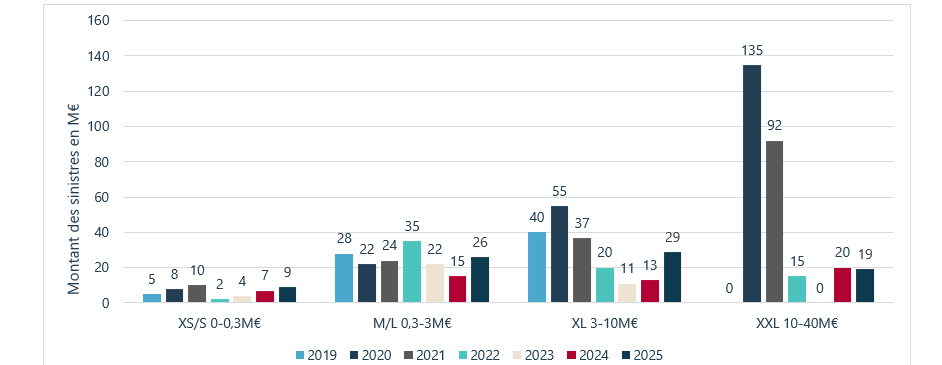
\includegraphics[width=0.80\textwidth]{figures_externes/lucy_taille_des_sinistres.png}
\caption{Charge indemnisée par classe de taille de sinistre, $2019$--$2025$. La classe la plus
haute est vide deux exercices sur sept : l'historique national s'arrête avant le haut de la
distribution.
Source : rapport LUCY 2026, Nexialog Consulting \citep{RapiorKaddouri2026}.}
\label{fig:lucy-taille}
\end{figure}

\section{Le règlement DORA}
\label{sec:dora}
% HARNAIS-HORS-SECTION: section reglementaire. Les seuls nombres sont des millesimes, des
% numeros d'articles et des references de textes, aucun ne provient d'un calcul du projet.

\subsection{Cadre réglementaire européen du cyber}
\label{subsec:cadre-reglementaire-europeen}
% HARNAIS-HORS-SECTION: section reglementaire. Les nombres sont la date d'entree en
% application, des millesimes et des numeros officiels de textes. Ce sont des donnees de droit.

Quatre textes européens encadrent le risque cyber. La directive NIS~2
\citep{NIS2Directive2022}, relative à la sécurité des réseaux et des systèmes d'information, impose
des exigences de sécurité et de notification aux entités essentielles et importantes. Elle rend
également l'organe de direction responsable des mesures de gestion du risque. Le règlement général
sur la protection des données \citep{RGPD2016} encadre les données personnelles, la directive sur la
résilience des entités critiques \citep{REC2022} la continuité des fonctions sociétales vitales. Le
règlement sur la cyberrésilience \citep{CRA2024} couvre enfin la sécurité des produits numériques.
Aucun n'est propre au secteur financier.

Le règlement DORA \citep{DORA2022} comble ce manque. Entré en application le $17$ janvier $2025$, il
s'adresse à une vingtaine de catégories d'entités financières, dont les entreprises d'assurance, et
leur demande de résister à l'incident, d'y réagir et de s'en rétablir. 

Nous ne modélisons que DORA, car il est le seul de ces textes à découper la résilience en piliers
dont la défaillance pourra se lire dans les incidents notifiés. Les cadres de l'intelligence
artificielle et de l'identité numérique ne sont pas traités. Le règlement sur la cyberrésilience,
applicable à partir de décembre~$2027$, agira sur la fréquence future des vulnérabilités. Notre calibration l'estime sur l'historique et ne la projette pas.

\subsection{Les cinq piliers de DORA}
\label{subsec:cinq-piliers-dora}
% HARNAIS-HORS-SECTION: section reglementaire. Les nombres sont les etiquettes P1 a P5, les
% numeros d'articles du reglement et les delais qu'il fixe. Ce sont des donnees de droit.

Le règlement organise la résilience en cinq domaines, notés P1 à P5, que nous appelons \emph{piliers}.
\begin{itemize}[leftmargin=1.4em,itemsep=2pt]
\item P1, gouvernance du risque lié aux technologies (articles~$5$ à~$16$) : responsabilité non
      délégable de l'organe de direction, cartographie des actifs et des dépendances critiques,
      contrôle interne continu.
\item P2, gestion, classification et notification des incidents (articles~$17$ à~$23$) : notification initiale dès que possible, sous quatre heures après classification majeure et au plus tard vingt-quatre heures après prise de connaissance. Si la classification intervient après ce délai, la notification suit sous quatre heures. Le rapport intermédiaire est dû sous soixante-douze heures après la notification initiale, le rapport final sous un mois après le rapport intermédiaire ou sa dernière mise à jour \citep{eu2025_301}.
\item P3, tests de résilience opérationnelle numérique (articles~$24$ à~$27$), dont des tests de
      pénétration guidés par la menace (TLPT), au moins tous les trois ans, pour les entités
      significatives (article~$26$).
\item P4, gestion du risque lié aux prestataires tiers (articles~$28$ à~$44$) : registre
      d'informations des contrats, clauses impératives de l'article~$30$, stratégie de sortie, et
      surveillance des prestataires critiques et prise en compte de leur chaîne de sous-traitance, sans limite générale au troisième rang.
\item P5, partage d'informations sur les cybermenaces (article~$45$), volontaire et encadré, le
      pilier le moins utilisable dans un calibrage actuariel.
\end{itemize}
Ces piliers ne sont pas indépendants, car un incident qui touche l'un dégrade la capacité de l'entité à tenir les autres (sous-section~\ref{subsec:chocs-cause-commune}). Nous formalisons cette dépendance au chapitre~\ref{chap:cascade}.

\subsection{Prestataires TIC, concentration et propagation du risque}
\label{subsec:risque-tiers-dora}
% SOURCES-SCRIPTS: 103

La sous-traitance informatique du secteur financier est concentrée sur un petit nombre de
fournisseurs, si bien qu'une défaillance chez l'un d'eux atteint de nombreuses entités sans faute de
leur part. DORA instaure pour cette raison une surveillance directe des prestataires critiques, ce qui
est nouveau dans l'architecture prudentielle européenne. Le premier bilan des notifications montre
le poids des prestataires. En $2025$, les sociétés de gestion ont adressé à l'Autorité des marchés
financiers $47$ notifications initiales, dont $31$ incidents majeurs confirmés, parmi lesquels $27$,
soit $87\,\%$, trouvent leur origine chez un prestataire \citep{amf2026incidents}.

Cette part dit d'où viennent les incidents ; elle ne fournit pas de probabilité de transfert entre piliers et ne calibre aucun paramètre du modèle. Les notifications initiales précèdent la confirmation du caractère majeur : l'écart avec les
incidents confirmés est celui d'un seuil de matérialité, et la collecte réglementaire ne retiendra que
les incidents au-dessus de ce seuil.

Pour la modélisation, l'exigence la plus utile est le registre d'informations. En recensant les
contrats TIC critiques et leurs chaînes de sous-traitance, il produit une donnée sur la concentration
technologique que l'évaluation interne des risques ne savait pas chiffrer. Il ne couvre que
la dépendance déclarée et ne dit rien de l'ordre dans lequel les défaillances s'enchaînent
(section~\ref{ch:livrable}). Les autorités de supervision ne publient pas de probabilité de
propagation entre piliers, si bien que les valeurs de propagation du modèle sont posées
à dire d'expert, puis bornées.

\section{Perception du risque et traitement prudentiel}
\label{sec:enjeu-prudentiel}

\subsection{Perception prospective selon France Assureurs et le CESIN}
\label{subsec:france-assureurs-cesin}
% SOURCES-SCRIPTS: 103 63

La cartographie prospective de France Assureurs classe le risque cyber au premier rang pour le
huitième exercice consécutif, avec un score de $4{,}1$ sur $5$ \citep{franceassureurs2026}. Ce score
a culminé à $4{,}48$ en $2022$ et revient à $4{,}10$ en $2026$ (figure~\ref{fig:carto-retro-rapport}).
Entre $2025$ et $2026$, il recule de $0{,}45$ point en fréquence anticipée et progresse de
$0{,}25$ point en sévérité.

D'après le baromètre du CESIN (Club des experts de la sécurité de l'information et du numérique), qui en donne le constat déclaré \citep{cesin2026}, $40\,\%$ des
entreprises interrogées ont subi au moins une cyberattaque significative en $2025$. L'hameçonnage
est cité par $55\,\%$ des entreprises attaquées, l'exploitation d'une faille par $41\,\%$ et l'attaque
indirecte par un tiers par $35\,\%$, part qui monte à $43\,\%$ dans les grandes entreprises. On
reconnaît là le pilier P4, vu par une source indépendante de ce travail.

Quatre entreprises attaquées sur cinq déclarent un impact sur leur activité, mais la sanction
d'une autorité ne concerne que $3\,\%$ des cas. Nous ne modélisons donc pas les pénalités : la
non-conformité coûte, dans le modèle, par les incidents qu'elle laisse passer. La déconnexion de l'entité par ses propres partenaires, citée dans $12\,\%$ des cas,
montre enfin que la dépendance joue dans les deux sens.

\begin{figure}[H]
\centering
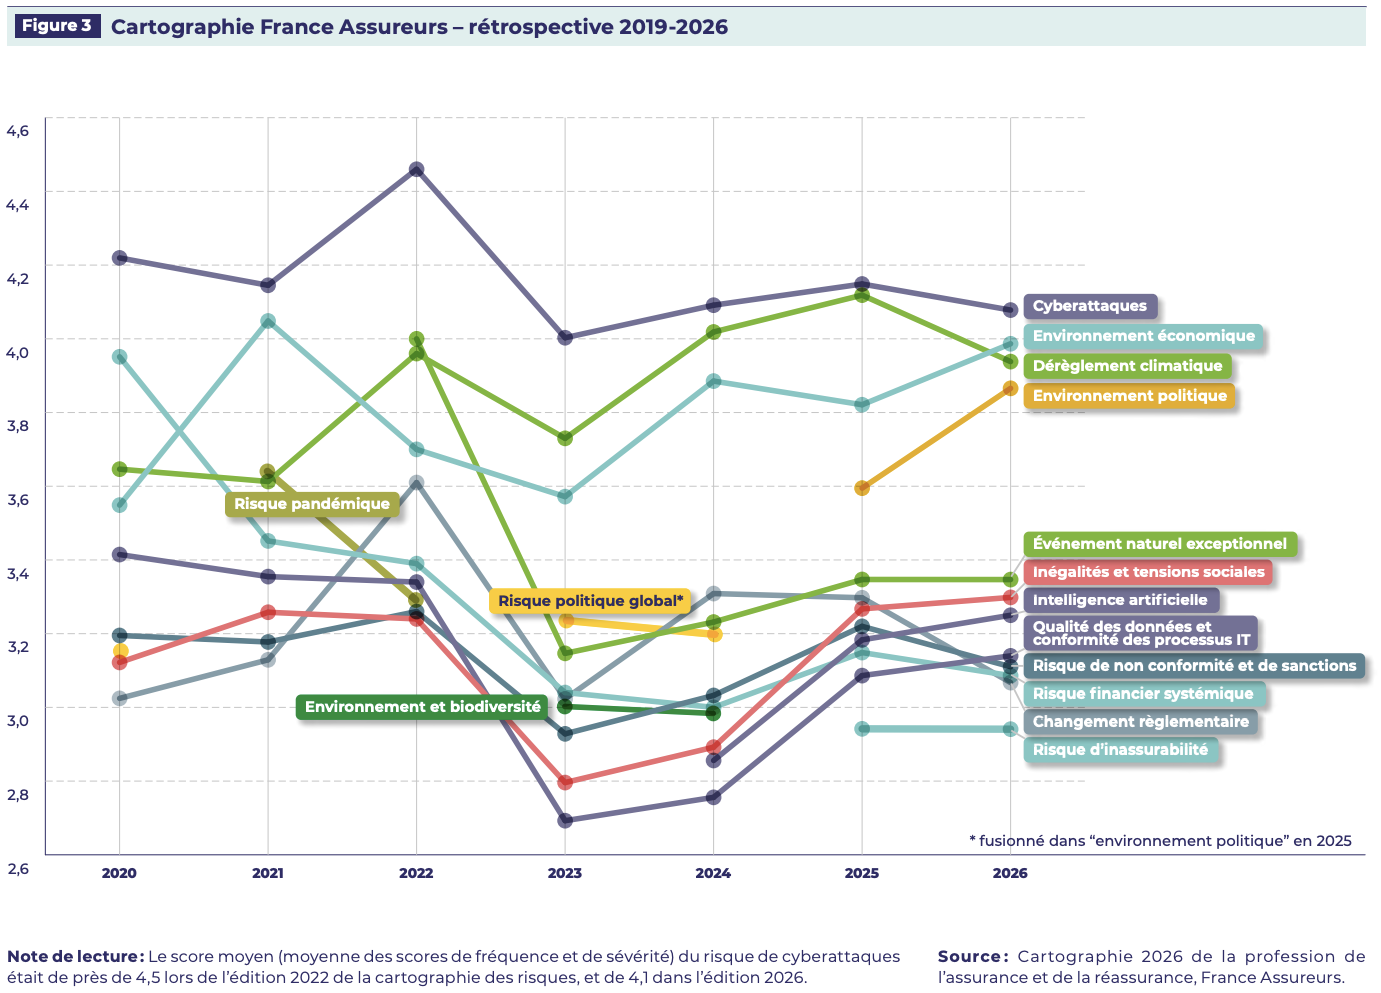
\includegraphics[width=0.72\textwidth]{figures_externes/carto_fa_2026_retrospective.png}
\caption{Trajectoire des scores de la cartographie prospective des risques de France Assureurs,
$2020$--$2026$. Le risque de cyberattaques reste au premier rang ; son score ne monte plus depuis
$2022$. Source : \citet{franceassureurs2026}.}
\label{fig:carto-retro-rapport}
\end{figure}

\subsection{Limites de Solvabilité II et de la Formule Standard}
\label{subsec:limites-formule-standard}
% HARNAIS-HORS-SECTION: section de cadrage prudentiel, aucune valeur chiffree du projet.

La Formule Standard de Solvabilité~II charge le risque opérationnel par un pourcentage de primes ou
de provisions techniques. Faute de
sous-module cyber, les assureurs sont renvoyés à leurs modèles internes et à leur évaluation interne
des risques (section~\ref{chap:reglementaire}).

Une copule, outil usuel, décrirait la loi jointe des pertes entre domaines, mais non l'ordre dans lequel un incident les atteint. Or deux matrices de dépendance transposées l'une de l'autre, que les statistiques
usuelles ne distinguent pas, conduisent en général à un capital différent
(chapitre~\ref{chap:cascade}).

\section{Cadre prudentiel et articulation avec DORA}
\label{chap:reglementaire}

% HARNAIS-HORS-SCRIPT: cadre reglementaire : numeros d'articles, delais de notification et seuils cites des textes (DORA, Solvabilite II, Bale). Ce sont des donnees de droit, pas des resultats.

Le risque opérationnel reçoit la même définition dans la banque et dans l'assurance. Il s'agit du
risque de perte résultant de l'inadaptation ou de la défaillance de procédures, de personnels et de
systèmes internes, ou d'événements extérieurs. Il comprend le risque juridique et exclut les risques
stratégique et de réputation.

Les modes de quantification ont cependant divergé. Le secteur bancaire a abandonné les
modèles internes de mesure avancée au profit d'une approche standardisée \citep{bcbs2017}, sans invalider l'approche
par distribution des pertes (LDA, \emph{Loss Distribution Approach}) comme outil de modélisation.
Nous en reprenons les deux marges, fréquence et sévérité, et remplaçons son agrégation par une
cascade dirigée. L'assurance conserve sous Solvabilité~II le choix entre la Formule Standard, des
paramètres propres à l'entreprise et un modèle interne, partiel ou global, approuvé par l'autorité de
contrôle.

Dans la Formule Standard, l'exigence pour risque opérationnel ($SCR_{Op}$) s'ajoute au capital de
solvabilité requis de base ($BSCR$), ajusté de la capacité d'absorption des pertes :
\begin{equation}
SCR = BSCR + Adj + SCR_{Op},
\qquad
SCR_{Op} = \min(0{,}3 \times BSCR,\ Op) + 0{,}25 \times Exp_{ul},
\label{reg:eq:scrop}
\end{equation}
où $Adj$ est l'ajustement pour la capacité d'absorption des pertes, $Exp_{ul}$ les frais annuels des contrats en unités de compte et $Op = \max(Op_{premiums}, Op_{provisions})$ applique des coefficients forfaitaires aux primes et
aux provisions. Cette forme est simplifiée, car l'article~204 du règlement délégué~2015/35 ajoute des
termes de croissance, de la forme $\max\!\left(0;\, 0{,}04 \times \Delta\!\right)$, qui pénalisent
les hausses de primes supérieures à $20\,\%$ d'un exercice à l'autre. Fondée sur des indicateurs de
volume, l'approche attribue la même exposition à deux assureurs de même volume, quelles que soient la
qualité de leur informatique et leur dépendance à des prestataires critiques. Le $SCR_{Op}$ réglementaire s'ajoute au BSCR sans diversification. Cela n'implique pas qu'un quantile ORSA supplémentaire doive être ajouté en entier : il faut éviter le double compte du risque informatique déjà couvert (\S\ref{sec:agregation-scr}).

Le $SCR_{Op}$ relève des exigences quantitatives (forfaitaires) de Solvabilité~II. Les exigences de gouvernance imposent l'évaluation
interne des risques et de la solvabilité (\emph{Own Risk and Solvency Assessment}, ORSA). Elle
confronte le profil de risque réel aux besoins de solvabilité et admet les scénarios stochastiques
que la Formule Standard ne produit pas. Notre modélisation se situe dans ce cadre. ORSA et DORA
partagent un objet, le risque opérationnel d'origine technologique, l'ORSA pour la continuité
financière, DORA pour la continuité opérationnelle. Nous partons d'états de conformité posés pour quantifier dans l'ORSA ce que celui-ci ne savait que décrire (chapitres~\ref{chap:multietats}
et~\ref{chap:resultats}).
                 % ex-chapitres 1 et 2
% =====================================================================
% VERSION ENSAE, REDUCTION SFE : chapitre 2, revue de littérature et positionnement.
% Phase 3 : copie a texte constant de chapitres/03_etat_art_positionnement.tex.
% Phase 4 (1er octobre 2026) : reecrit et condense ; toutes les citations, le tableau
% comparatif et les nombres sont conserves. Le texte d'origine reste dans chapitres/
% (version Institut) et dans l'historique Git.
% Lu par main_ensae.tex seul : ne jamais le faire lire par main_institut.tex,
% qui garde chapitres/.
% =====================================================================
\chapter{Revue de littérature et positionnement}
\label{ch:positionnement}

% SOURCES-SCRIPTS: 08g 32 01 23

La modélisation actuarielle du risque cyber s'est construite en trois vagues. La première traite
l'assurabilité du risque et la rareté des données \citep{BienerElingWirfs2015}, et décrit les
marges par la théorie des valeurs extrêmes. La deuxième modélise la contagion entre entités d'un
portefeuille par des modèles de réseau ou épidémiologiques, et la troisième décrit la dynamique des
arrivées par des processus de Hawkes.

Nous reprenons à ces travaux les marges empiriques et le cadre du risque extrême. Au risque de
crédit, nous empruntons le processus de branchement multitype pour la propagation entre piliers
(chapitre~\ref{chap:cascade}), et les modèles multi-états de migration de rating pour l'état de
conformité (chapitre~\ref{chap:multietats}). 

\section{Dépendance dirigée et dépendance à l'ordre}
% SOURCES-SCRIPTS: 08g 32 01 23

La matrice $W$ de contagion entre piliers (posée à dire d'expert, puis bornée au chapitre~\ref{chap:partielle}) donne par $W_{jk}$ la propension d'une défaillance de $j$ à entraîner celle de $k$. La ligne désigne l'émetteur, la colonne le récepteur. Elle est
dirigée, au sens où $W_{jk}\neq W_{kj}$, et autorise des cycles comme P1$\to$P2$\to\cdots\to$P1. La
normalisation de Leontief permet de stabiliser ces cycles ($\rho(W)\le g<1$, forme réduite $(I-W)^{-1}$).

Avec le score de criticité du modèle, de $0$ à $10$ et construit sur $W$ (chapitre~\ref{chap:cascade}), $22$ des $26$ sous-ensembles d'au moins deux piliers changent de score selon l'ordre. L'écart atteint $6$ points, entre $8$ pour la chaîne P1$\to$P2 et $2$ pour la chaîne
P2$\to$P1. Un score statique invariant par permutation ne peut pas
reproduire cette propriété. Nous avons aussi testé, sous trois formulations, une non-transitivité de la dominance entre piliers ; elle ne se vérifie pas et n'est pas revendiquée (chapitre~\ref{chap:cascade}).

\section{Comparaison aux approches existantes}
% SOURCES-SCRIPTS: 32 23 01

\begin{center}\footnotesize
\renewcommand{\arraystretch}{1.35}
\begin{tabular}{@{}p{3.1cm} c c c c p{3.1cm} p{2.9cm}@{}}
\toprule
\textbf{Approche} & \textbf{Dirigée} & \textbf{Ordre} & \textbf{Cycles} & \textbf{Propagation} &
\textbf{Donnée requise} & \textbf{Objet modélisé} \\
\midrule
Matrices de risque / AMDEC & \non & \non & \non & \non & dires d'expert & risques listés (probabilité $\times$ gravité) \\
Copule (Gumbel, gaussienne) & \non & \non & \non & \non & co-mouvement observé & briques de perte \\
Réseau / épidémiologie (SIR) & \oui & \non & \oui & \oui & structure réseau $+$ taux d'infection & entités d'un portefeuille \\
Hawkes (multivarié) & \oui & \non & \oui & \oui & horodatage fin des arrivées & types d'attaque, dans le temps \\
Réseau bayésien & \oui & \non & \non & \oui & tables de probabilités conditionnelles & variables d'un graphe acyclique \\
\cascell\textbf{Cascade dirigée (ici)} & \cascell\oui & \cascell\oui & \cascell\oui & \cascell\oui & \cascell jugement d'expert, puis bornes & \cascell\textbf{domaines de contrôle (piliers) d'une entité} \\
\bottomrule
\end{tabular}
\end{center}

\vspace{2pt}
\noindent Les matrices de risque et l'analyse des modes de défaillance, de leurs effets et de leur
criticité (AMDEC), standard des praticiens, notent des risques sans propagation ni direction.
L'AMDEC les classe par un indice de priorité (RPN $=$ gravité $\times$ occurrence $\times$ détection). Les copules
\citep{BohmeKataria2006, HerathHerath2011} décrivent une dépendance statique entre risques, sans ordre d'atteinte. Dans la comparaison du chapitre~\ref{chap:resultats}, leur interaction moyenne entre piliers est nulle par construction ($+0$), contre $+560$~M\euro{} (périmètre financier étudié) pour la cascade. Leur ordre de priorité diffère de celui de la cascade sur P2 et P3 (chapitre~\ref{chap:resultats}).

Les modèles de réseau et épidémiologiques \citep{HillairetLopez2021,
HillairetLopezDOultremontSpoorenberg2022, XuHua2017, Baldwin2017} modélisent la contagion entre
entités d'un portefeuille et exigent la structure du réseau et des taux d'infection, indisponibles
ici. Nous reprenons cependant à Hillairet et Lopez l'idée d'états successifs, transposée à l'état de conformité de chaque pilier. Les processus de Hawkes \citep{BessyRolandBoumezouedHillairet2021, BoumezouedCherkaouiHillairet2023}
décrivent l'auto-excitation entre types d'attaque. Sur le nombre annuel d'incidents, les données ne séparent pas l'auto-excitation d'une co-occurrence exogène le même jour (chapitre~\ref{ch:robustesse}). Nous retenons la seconde lecture, plus parcimonieuse ; elle se distingue du modèle à deux phases de $2023$, qui conserve l'auto-excitation tout en ajoutant une excitation externe. Les réseaux bayésiens intègrent la direction, mais supposent un graphe acyclique
et des probabilités conditionnelles qui se heurtent au même problème d'identification que $W$
(chapitre~\ref{ch:identifiabilite}).

\section{Travaux par thème}

\subsection*{Dépendance et contagion}
% SOURCES-SCRIPTS: 08g
La corrélation entre risques cyber a d'abord été traitée par
copules \citep{BohmeKataria2006, HerathHerath2011}. Sur la chronologie PRC, l'indice de Gini de la charge journalière vaut $0{,}69$ ($2\,922$ jours, $4\,614$ événements) : les sinistres se concentrent sur peu de jours, ce qui est compatible avec une accumulation par cause commune.
\citet{HillairetLopez2021} couplent des processus de comptage à un modèle épidémiologique
compartimental de type SIR (susceptibles, infectés, rétablis), et \citet{HillairetLopezDOultremontSpoorenberg2022} y ajoutent une
structure de réseau. \citet{XuHua2017} et \citet{Baldwin2017} modélisent la contagion entre cibles.

\subsection*{Dynamique temporelle}
\citet{BessyRolandBoumezouedHillairet2021} ajustent des processus de
Hawkes aux données PRC, l'une de nos sources, puis \citet{BoumezouedCherkaouiHillairet2023}
ajoutent un terme exogène. \citet{HillairetReveillacRosenbaum2021} en développent la théorie pour le
pricing de dérivés, et \citet{Peng2016} les appliquent à des taux d'attaque horodatés.

\subsection*{Fréquence, sévérité et queue}
\citet{Edwards2016} ajustent une binomiale négative au
nombre journalier de brèches, et \citet{LuZhangZhu2024} séparent fréquence et nombre de brèches par
événement, une structure compatible avec la loi de fréquence retenue ici (binomiale négative, chapitre~\ref{chap:socle}). \citet{FarkasLopezThomas2021}
tarifent par arbres de régression GPD. La queue lourde des pertes cyber est documentée
\citep{MaillartSornette2010, wheatley2016}, et \citet{elingloperfido2017} comparent plusieurs
familles de lois sur les brèches de données. \citet{elingwirfs2019} étudient les pertes cyber de la
base SAS OpRisk Global par les valeurs extrêmes, et leur étude est le précédent le plus proche pour la sévérité.

\subsection*{Travaux sur les mêmes sources}
\citet{Ranguin2024} modélise le risque cyber des
entreprises françaises pour la Caisse Centrale de Réassurance, à partir de PRC, VCDB, Hackmageddon et
de l'étude LUCY. La sévérité y est construite par arbres de régression GPD sur le volume de données
compromises. La sinistralité d'un portefeuille fictif est simulée, sinistres courants compris. Les lois
sont ensuite reparamétrées dans un cadre bayésien sur le marché français. Cette étude ne produit pas de
mesure de capital à un quantile réglementaire. Notre objet est le besoin de capital d'une
entité financière selon son état de conformité. Nous calibrons la sévérité sur des pertes en montants et
modélisons la dépendance entre piliers.

Sur PRC, \citet{KherLopezRapior2023} estiment la gravité d'un incident à partir de sa description
textuelle par réseaux de neurones, et \citet{Dountio2026} prolonge cette démarche. Ces travaux
classent la sévérité d'un incident en volume de dossiers compromis.

\subsection*{Cadre structurel et identification partielle}
Le facteur latent commun vient du modèle à facteur de \citet{Vasicek2002}, et la normalisation qui stabilise une contagion avec
cycles provient de l'analyse entrées-sorties de \citet{Leontief1936}.

Le traitement du paramètre non identifiable relève de la littérature économétrique des bornes. On y
caractérise l'ensemble des valeurs compatibles avec les données, et l'on en déduit un intervalle pour
la quantité d'intérêt. Initiée par les bornes de sélection de \citet{Manski1990}, exposée dans
\citet{Manski1995} et systématisée par \citet{Tamer2010}, cette approche est courante en évaluation
des politiques publiques. Elle est presque absente de l'actuariat du cyber, où l'on pose d'ordinaire
un paramètre non observable à dire d'expert. Nous publions le capital en bornes sur l'ensemble admissible
(chapitre~\ref{chap:partielle}). Une échelle de repli sur l'écart $u_{ij}$ à la dépendance moyenne y gradue les hypothèses de
structure.

\subsection*{Cascade de risques climatiques}
Un préprint de 2026 propose un réseau de cascade pour le
risque climatique de catastrophe \citep{ccrn2026}, sans péril, données ni auteurs communs avec ce
travail. Il s'agit d'un graphe dirigé de propagation entre n\oe uds, avec des indices de temps
séparés. Ce préprint est synthétique, et ses auteurs mettent en garde contre toute lecture de ses
valeurs comme calibrées. Nous n'en reprenons aucun chiffre ; nous empruntons l'architecture : séparation d'échelles, protocole de comparaison, expérience d'ablation et forme
fonctionnelle.

\section{Positionnement}

Nous reprenons la queue de sévérité par les valeurs extrêmes, la structure de paquet de la fréquence
et l'idée d'états successifs de Hillairet et Lopez, transposée à la conformité. Deux éléments sont nouveaux : une
dépendance dirigée et à l'ordre entre les piliers DORA, traduite en capital, et une frontière
d'identifiabilité explicite, traduite en recommandation sur les données à déclarer. Aucune des références que nous avons lues ne modélise une dépendance dirigée entre piliers d'une entité ni ne la traduit en besoin de capital (ORSA). Les lois de sévérité et de fréquence sont reprises de la littérature et calibrées.

\nocite{BohmeKataria2006, HerathHerath2011, HillairetLopez2021,
  HillairetLopezDOultremontSpoorenberg2022, XuHua2017, Baldwin2017,
  BessyRolandBoumezouedHillairet2021, BoumezouedCherkaouiHillairet2023,
  HillairetReveillacRosenbaum2021, Peng2016, Edwards2016, LuZhangZhu2024,
  FarkasLopezThomas2021, Vasicek2002, Leontief1936}
                    % ex-3
% =====================================================================
% VERSION ENSAE, REDUCTION SFE (phase 3, 1er octobre 2026) : chapitre 3, donnees.
% Copie a texte constant de chapitres/05_donnees_limites.tex.
% Ne changent que les titres et les renvois repares, listes dans
% reduction/phase3.md.
% Lu par main_ensae.tex seul : ne jamais le faire lire par main_institut.tex,
% qui garde chapitres/.
% =====================================================================

\chapter{Données}
\label{chap:donnees}
\label{part:donnees}

% MIGRÉ AUTOMATIQUEMENT depuis memoire/main.tex (plages 1002-1433).
% Hiérarchie descendue d'un cran, labels préfixés "don:".
% RELECTURE FAITE (août 2026). Aucune phrase du chapitre n'annonce la copule ni
% la variable latente comme LE modèle. Ajouts d'août : la table des trois
% fréquences, le seuil de collecte, et la section des deux biais chiffrés
% (élasticité de taille corrigée par troncature, chain-ladder de remontée).
%==============================================================

Trois bases alimentent le modèle, chacune pour la composante qu'elle peut renseigner.

%--------------------------------------------------------------
%--------------------------------------------------------------
\section{Sources et rôles}
\label{sec:carto}
%--------------------------------------------------------------

\begin{center}
\renewcommand{\arraystretch}{1.3}
\begin{tabular}{>{\raggedright}p{2.75cm} >{\raggedright}p{2.6cm} >{\raggedright}p{3.9cm} >{\raggedright\arraybackslash}p{4.05cm}}
\toprule
\rowcolor{lightblue}
\textbf{Source} & \textbf{Effectif retenu} & \textbf{Rôle dans le modèle} & \textbf{Justification / limite} \\
\midrule
PRC 2025 & $15\,053$ incidents, 2019 à 2025 & Sévérité alternative via conversion Jacobs ; nombre annuel de notifications $\lambda_{ref}$, décrit et non utilisé par le moteur &
Périmètre défini, mais sévérité dérivée d'un modèle log-log \\
\addlinespace
SAS OpRisk Global & $41\,975$ pertes, dont $582$ en cyber $\times$ finance, 1979 à 2026 & Sévérité (montants réels) et nombre annuel d'incidents du moteur ($\lambda$) &
Montants observés, mais biais vers les grandes entités financières \\
\addlinespace
Hackmageddon & $1\,041$ incidents, premier semestre 2026 & Parts par vecteur d'attaque (structure du risque) &
Ne fixe aucun niveau : pondère le multiplicateur qui fait passer $\lambda$ d'un état de conformité à l'autre \\
\bottomrule
\end{tabular}
\end{center}

Les articles~19 et~231 du règlement délégué (UE) 2015/35 exigent des données exactes, exhaustives et
appropriées, pour les provisions techniques et pour un modèle interne ; nous prenons ces critères pour référence. Aucune des bases que nous avons examinées ne remplit ces trois exigences. Nous documentons les biais de chaque source et leurs retraitements.

% SOURCES-SCRIPTS: 63 104

\section{Biais statistiques des sources}
\label{sec:trois-biais}

Trois biais affectent les bases PRC et OpRisk. Le
\emph{biais de sélection} touche OpRisk, qui recense surtout des pertes rendues publiques, donc
celles des grandes entités ou des montants exceptionnels. Il surreprésente les événements extrêmes,
et nous ramenons la fréquence et la sévérité à la taille de l'entité par deux élasticités estimées
(\S\ref{sec:biais-chiffres} et chapitre~\ref{chap:resultats}). Le \emph{biais de déclaration}
touche la PRC, car la notification des fuites de données personnelles est obligatoire dans la plupart
des États américains, pas celle d'un rançongiciel qui n'exfiltre rien. Le niveau de fréquence est
donc lu sur OpRisk, et la répartition par vecteur sur Hackmageddon.

Un \emph{biais de survie} pourrait sous-représenter les entités disparues, mais les pertes qui ont conduit à une faillite sont souvent publiques : ni son existence ni son signe ne sont établis sur ces bases, et il ne figure pas parmi les écarts mesurés du chapitre~\ref{ch:robustesse}.

\section{Hétérogénéité temporelle et actualisation des sinistres}

Le sous-échantillon cyber-finance OpRisk contient des pertes de $1979$ à $2026$, période sur laquelle les montants nominaux dérivent.
Pour chaque perte, la base donne le montant de l'année de l'événement et sa valeur courante, corrigée
de l'inflation générale. Leur rapport, égal à un pour les années récentes, atteint $1{,}747$ en
$2004$, d'où une inflation implicite de $2{,}19\,\%$ par an. Nous calibrons cependant sur le premier,
c'est-à-dire sur des montants \emph{nominaux}. Ce choix minore les sinistres anciens ramenés en euros
courants, donc la queue et le capital. Son effet sur la dérive des pertes est mesuré au
\S\ref{soc:sec:backtest}.
% SOURCES-SCRIPTS: 102

La PRC fournit la fréquence de référence $\lambda_{ref}$, qui compte des notifications sans seuil de
matérialité et ne fixe pas le niveau du capital. Elle sert aussi de source de sévérité indirecte : la conversion de \citet{jacobs2014}, $\ln(L) = 7{,}68 + 0{,}76\,\ln(X)$, donne la perte $L$ en dollars d'un incident à partir de son nombre $X$ d'enregistrements. Calibrée sur les $15\,053$ incidents 2019--2025 dont le volume touché est renseigné (la figure~\ref{fig:composition-temporelle-rapport} compte toutes les notifications), la queue PRC a un paramètre de forme $\hat{\xi}_{\text{PRC}} = 1{,}03$ (intervalle à $90\,\%$ :
$[0{,}97~;~1{,}09]$). À cette valeur, l'espérance est infinie. On ne la lit qu'avec le plafond de sévérité
propre à cette source \matcomp.

\begin{figure}[H]
\centering
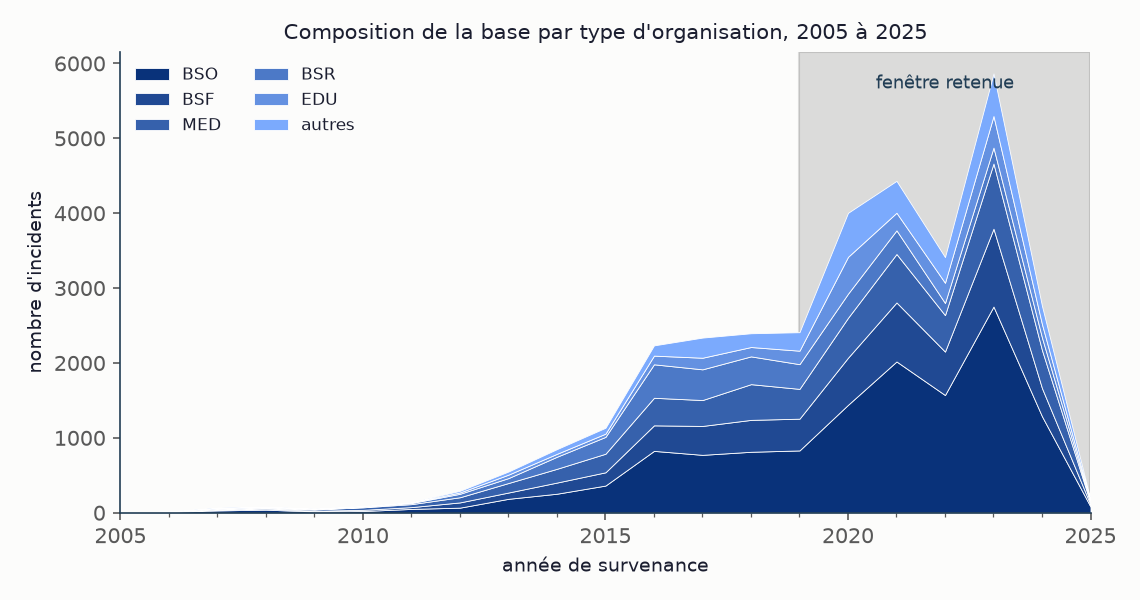
\includegraphics[width=0.78\textwidth]{D4_composition_temporelle.png}
\caption{Composition de la chronologie PRC par type d'organisation et par année. La zone grisée est
la fenêtre retenue. La hausse d'avant $2019$ suit l'extension de la collecte. La baisse de $2025$ traduit le manque de recul. BSF : organisations financières ; les autres codes sont ceux de la base.}
% SOURCES-SCRIPTS: 104
\label{fig:composition-temporelle-rapport}
\end{figure}



% SOURCES-SCRIPTS: 57 62 63

\section{Fréquences et seuils de collecte}

% SOURCES-SCRIPTS: 08b 60 62

La valeur de la fréquence dépend du périmètre de comptage de la source. Sur le
panel firme-année du SAS OpRisk (sous-catégories TIC, 2005--2022), le taux est de $0{,}10$ événement
par firme et par an toutes firmes confondues, et $0{,}21$ pour les firmes à au moins dix événements.
Au chapitre~\ref{chap:resultats}, nous estimons $\lambda$ comme une fonction de la taille de firme afin
de le lire à celle de l'entité notionnelle, ce qui donne $0{,}092$. Ces taux sont par firme ; celui du moteur compte le périmètre financier étudié. Le panel d'entité retient cinq sous-catégories TIC, plus larges que le filtre cyber-finance de sévérité : leur réconciliation reste nécessaire. Tous ne retiennent que les pertes au-dessus du seuil de collecte d'OpRisk. Ils comptent
donc les incidents TIC \emph{matériels}, pas tous les incidents au sens du reporting DORA.

Le taux par firme est une propriété d'entité, lisible sur un panel. Le tableau~\ref{tab:echelle} traduit ces échelles en capital.

Le terme de fréquence recouvre trois taux, à trois niveaux d'observation :
\begin{center}\small
\renewcommand{\arraystretch}{1.3}
\begin{tabular}{@{}l l r p{5.1cm}@{}}
\toprule
\textbf{Symbole} & \textbf{Source} & \textbf{Valeur} & \textbf{Ce qu'il compte} \\
\midrule
$\lambda_{ref}$ & PRC & $341$/an & notifications de violation de données des
\emph{organisations financières} de la base PRC (code \texttt{BSF}), et non de la base
entière, qui en compte $2\,150$ par an. Décomposée par vecteur d'attaque ; n'entre pas dans le moteur et ne fixe aucun niveau de capital. \\
$\lambda$ & OpRisk & $21{,}6$/an & incidents TIC \emph{matériels} du secteur
financier mondial. C'est l'entrée du moteur de cascade et le seul des trois dont dépend le capital. \\
$\lambda_{\text{entité}}$ & OpRisk & $0{,}092$/an & les événements TIC du panel, rapportés
à \emph{une} firme et lus \emph{à la taille} de l'entité notionnelle. C'est
l'échelle de lecture d'une entité soumise à DORA. \\
\bottomrule
\end{tabular}
\end{center}
Le facteur $3\,719$ entre $\lambda_{ref}$ et $\lambda_{\text{entité}}$ sépare trois comptages, ceux des notifications, des pertes
matérielles du secteur et des pertes matérielles par entité. Le moteur de simulation n'utilise que
$\lambda$.
% SOURCES-SCRIPTS: 67

\section{Effet chiffré de deux biais}
\label{sec:biais-chiffres}
% SOURCES-SCRIPTS: 57

Corrigée de la troncature au seuil de collecte, l'élasticité de la sévérité à la taille est de
$b=0{,}087$, et la sévérité transposée à l'entité notionnelle n'est multipliée que par $0{,}861$. Le
biais de taille est réel, mais faible. On corrige la troncature à droite par chain-ladder : les $97$ événements observés sur 2023--2025 deviennent $255$ à l'ultime, soit $85{,}0$ par an contre $74{,}1$ sur 2015--2022, et la fréquence est relevée d'un facteur $1{,}147$. Le risque TIC n'a donc pas
baissé après 2022, il n'est pas encore remonté dans la base. Les régressions et le triangle de
développement sont déportés \matcomp.
% SOURCES-SCRIPTS: 67

Les deux corrections se compensent presque sur la perte moyenne, $0{,}861\times1{,}147=0{,}987$, soit
un effet net de $1{,}3\,\%$, inférieur à l'incertitude d'estimation de chacune, mais elles ne se compensent pas sur le capital. À queue lourde, le quantile à $99{,}5\,\%$ répond à la sévérité bien plus qu'à la fréquence. Leur effet net sur le capital n'est pas chiffré. La correction de taille agit sur la sévérité et celle de troncature sur la fréquence ; leur compensation sur la moyenne ne détermine pas le signe de l'effet sur le quantile.

\section{Hackmageddon et la structure du risque}
\label{sec:hackmageddon}

Hackmageddon donne la \emph{structure} du risque, jamais son niveau. Le décompte retenu couvre le
semestre janvier--juin 2026, avec 1\,041 incidents, dont 840 à vecteur d'accès initial identifié
($81\,\%$). Le jeu consulté n'a pas été conservé ; relu en octobre 2026 avec une autre grille, il ne redonne pas ces décomptes à l'unité. Ce sont des citations datées. Ils fixent les parts de répartition par vecteur, qui pondèrent le
multiplicateur de fréquence entre états de conformité (\S\ref{sec:quatre-canaux}). Ce
multiplicateur hérite donc de leur statut de citation.

\begin{center}
\renewcommand{\arraystretch}{1.3}
\begin{tabular}{>{\raggedright}p{5cm} c >{\raggedright\arraybackslash}p{6cm}}
\toprule
\rowcolor{lightblue}
\textbf{Vecteur d'attaque} & \textbf{Part} & \textbf{Exigence DORA} \\
\midrule
Hameçonnage / ingénierie sociale & $38{,}8\,\%$ & Art.~13, sensibilisation \& formation \\
Exploitation vuln.\ exposée & $33{,}8\,\%$ & Art.~26, tests TLPT ; Art.~8--10 \\
Chaîne d'approvisionnement / tiers TIC & $15{,}8\,\%$ & Art.~28--44, gestion du risque tiers \\
Identifiants compromis & $6{,}3\,\%$ & Art.~9, contrôle d'accès \& MFA \\
\bottomrule
\end{tabular}
\end{center}

Deux parts structurent les scénarios du chapitre~\ref{chap:multietats} : $15{,}8\,\%$ des attaques
empruntent le vecteur tiers, objet des articles~28 à~44, et $49{,}6\,\%$ (dont ces $15{,}8\,\%$) relèvent de vecteurs qu'un
test TLPT est censé détecter en amont. La base recense des incidents rendus publics, ce qui interdit
d'en tirer un niveau de fréquence, et sa taxonomie est instable. La catégorie rançongiciel n'existait
pas en 2023, et une lecture naïve lui prête une hausse de 11 points là où, après reclassement, elle recule de 23 points. Seules les motivations se comparent directement dans le temps. Les catégories bâloises de la base SAS informent trop faiblement la sévérité pour fonder une segmentation (\S\ref{sec:profilage-variables}).

% SOURCES-SCRIPTS: 63

\section{OpRisk Global et la sévérité en euros}
\label{sec:oprisk}

% SOURCES-SCRIPTS: 07 47 63

OpRisk Global est la base de référence historique du risque opérationnel au sens de Bâle. Le risque cyber y est reconstruit à
partir des catégories \og Systems Security\fg{} et \og Business Disruption and System Failures\fg{}, et
le périmètre cyber $\times$ finance compte 582 incidents, dont certains sont antérieurs à 2000. Le dénominateur de 27 ans utilisé pour la fréquence est une convention de calibration ; il ne correspond pas à toute la période observée. Une recalibration cohérente du filtre temporel et de la fréquence reste nécessaire. \citet{elingwirfs2019}
en extraient également les pertes d'origine informatique. Cette base alimentait les modèles internes de
mesure avancée (section~\ref{chap:reglementaire}), qui calibraient la sévérité extrême sur des pertes
observées sans passer par un indicateur de volume. Nous reprenons cette logique.

Sur la population de la fréquence (secteur financier, catégories TIC, 2005--2022, $1\,476$
observations), la sévérité se décrit ainsi :
\begin{center}
\renewcommand{\arraystretch}{1.3}
\begin{tabular}{l r l r}
\toprule
\rowcolor{lightblue}
\textbf{Indicateur} & \textbf{Valeur} & \textbf{Indicateur} & \textbf{Valeur} \\
\midrule
Médiane & 1{,}20 M\$ & P99 & 419{,}3 M\$ \\
Moyenne & 33{,}8 M\$ & Maximum & 10\,970{,}8 M\$ \\
P90 & 25{,}3 M\$ & Total cumulé & 49{,}8 Md\$ \\
\bottomrule
\end{tabular}
\end{center}
Les montants de ce tableau sont en dollars ; le moteur les convertit en euros au taux fixe de $0{,}92$. Le décile supérieur concentre $92{,}3\,\%$ de la perte totale et le centile supérieur $65{,}1\,\%$,
ce qui justifie la théorie des valeurs extrêmes du chapitre~\ref{chap:socle}.
% SOURCES-SCRIPTS: 67

Nous ajustons la loi de Pareto généralisée sur les $582$ pertes cyber $\times$ finance au-delà d'un
seuil $u = 20$~M\euro, proche du percentile~85 des montants, où le graphique des excès moyens devient
linéaire (figure au supplément, \S\ref{don:fig:mep}). Avec $91$ excès, on obtient :
\[
\hat{\xi} = 0{,}595 \quad (\text{IC}_{90\%}=[0{,}30\,;\,0{,}83]), \qquad
\hat{\sigma} = 58{,}0~\text{M\euro}, \qquad
\qsev_{99{,}5\%}(X) = 663~\text{M\euro}.
\]
Le dernier terme est le quantile de la sévérité d'un sinistre, pas un capital, car le besoin de capital
est le quantile de la charge annuelle agrégée, obtenu par composition avec la fréquence. L'intervalle
bootstrap de ce quantile, $[411\,;\,1037]$~M\euro, couvre un facteur~2{,}5. L'écart avec la PRC
($\hat{\xi}_{\text{PRC}} = 1{,}03$) ne mesure pas une différence de risque : la sévérité PRC
est une puissance de pente $0{,}76$ du nombre d'enregistrements, et une puissance multiplie l'indice
de queue par son exposant. Les deux indices sont positifs ($\xi > 0$), sur deux objets différents.

%--------------------------------------------------------------
\section{Analyse exploratoire et profilage des variables}
\label{sec:profilage-variables}
%--------------------------------------------------------------
% SOURCES-SCRIPTS: 104

Le profilage des variables des deux bases, détaillé dans le supplément, montre d'abord que, dans la
chronologie PRC, un champ non renseigné prend la valeur \texttt{UNKN} au lieu d'être vide. Le nombre d'enregistrements touchés n'est ainsi documenté que dans $41{,}77\,\%$ des cas. De plus, la base n'agrège pas les
notifications, si bien qu'un même incident déclaré à plusieurs autorités y figure plusieurs fois. La
déduplication retire $1\,643$ lignes, soit $10{,}9\,\%$ des lignes, une borne basse. Nous n'additionnons jamais ces volumes, mais les doublons pèsent encore sur les comptages et sur l'ajustement de la sévérité ; leur effet n'est pas chiffré.

La chronologie PRC compte $74\,783$ incidents, dont $31\,217$ documentent un volume touché
positif. La base SAS compte $41\,976$ lignes brutes et $41\,975$ pertes après retrait d'une
aberration de saisie, dont $1\,099$ en catégories TIC et $582$ dans le croisement cyber $\times$
finance retenu pour la sévérité. Le tableau donne pour chaque variable son type, son rôle et la part
de lignes renseignées, \texttt{UNKN} compté comme un manquant.

\begin{center}\footnotesize
\renewcommand{\arraystretch}{1.05}
\begin{tabular}{@{}>{\ttfamily\raggedright}p{3.35cm} l >{\raggedright}p{5.1cm} l r@{}}
\toprule
\textbf{Variable} & \textbf{Type} & \textbf{Rôle dans le modèle} & \textbf{Base} & \textbf{Renseignée} \\
\midrule
total\_affected & quantitative & enregistrements touchés, seule mesure d'impact de la base & PRC & $41{,}77\,\%$ \\
residents\_affected & quantitative & sous-ensemble territorialisé du précédent & PRC & $79{,}88\,\%$ \\
breach\_date & temporelle & date de survenance, support de la fréquence annuelle & PRC & $54{,}82\,\%$ \\
reported\_date & temporelle & date de notification, support du délai de détection & PRC & $99{,}54\,\%$ \\
end\_breach\_date & temporelle & fin d'exposition, support de la durée d'incident & PRC & $28{,}18\,\%$ \\
organization\_type & qualitative & classe d'organisation, huit modalités & PRC & $89{,}29\,\%$ \\
breach\_type & qualitative & vecteur de la brèche, huit modalités & PRC & $47{,}31\,\%$ \\
\midrule
Loss Amount & quantitative & montant de perte avérée, source de la sévérité & SAS & $100\,\%$ \\
Event Risk Category & qualitative & catégorie bâloise de niveau 1, sept modalités & SAS & $100\,\%$ \\
Sub Risk Category & qualitative & sous-catégorie, définit le périmètre TIC & SAS & $100\,\%$ \\
Basel Business Line & qualitative & ligne métier, dix modalités & SAS & $100\,\%$ \\
Industry Sector Name & qualitative & secteur, définit le périmètre financier & SAS & $100\,\%$ \\
Revenue & quantitative & chiffre d'affaires, mesure de taille & SAS & $87{,}82\,\%$ \\
Assets & quantitative & actif total, mesure de taille prudentielle & SAS & $83{,}51\,\%$ \\
\bottomrule
\end{tabular}
\end{center}

Le volume touché est la variable d'impact la moins bien renseignée, et pas au hasard : les champs
qu'impose l'obligation de notification sont remplis, ceux qui demandent une enquête ne le sont pas.
Le manquant est donc plausiblement corrélé à la gravité, ce qui explique que le modèle ne conditionne
la sévérité sur aucune de ces variables.

La perte n'est ni normale ni log-normale. Après passage au logarithme, le test de Shapiro-Wilk rejette encore la normalité (statistique $W=0{,}970$ sur les enregistrements PRC, $W=0{,}986$ sur les pertes SAS). Nous modélisons donc la seule queue, par une loi de Pareto généralisée au-delà d'un seuil.

Sur $33\,769$ pertes à profil financier complet, le $V$ de Cramér reste sous $0{,}20$,
l'$\varepsilon^2$ de Kruskal-Wallis sous $0{,}08$, et les corrélations de rang entre perte et taille
sous $0{,}16$. Ces tailles d'effet sont faibles, et nous ajustons une queue commune. C'est une hypothèse : l'indice varie selon la catégorie bâloise, et aucune base n'observe la sévérité par pilier. L'actif
total est le moins lié à la perte des trois mesures de taille ($0{,}068$, contre $0{,}159$ pour le
chiffre d'affaires et $0{,}139$ pour l'effectif). La mise à l'échelle du chapitre~\ref{chap:resultats} utilise pourtant le bilan, le prédicteur le plus faible des trois ; c'est une hypothèse du modèle.

\section{Limites des données}
\label{sec:portee-donnees}

Les pertes observées donnent une fréquence d'incidents, modulée entre états de conformité selon la répartition des attaques citée. Elles servent aussi à calibrer une
sévérité de queue lourde sur OpRisk, à la confronter à une source indépendante et à traiter l'écart
entre sources comme une incertitude à part entière.

Ces données ne mesurent pas la conformité DORA d'une entité ; nous posons donc l'état de chaque pilier (chapitre~\ref{chap:multietats}). Il
n'existe pas de base d'incidents harmonisée, exhaustive et exempte de biais de visibilité. Faute
d'historique d'événements joints, on ne peut pas estimer la corrélation entre les pertes des piliers, que
nous traitons au chapitre~\ref{chap:cascade} par une structure de dépendance explicite. Le registre des incidents majeurs que DORA instaure atténuera ces limites sans les lever : limité aux incidents au-dessus d'un seuil de matérialité, il restera tronqué.

S'il renseigne la taille de l'entité et le prestataire en cause, il permettra de conditionner la sévérité à la taille et cartographiera les prestataires tiers ; l'effet d'une telle donnée sur le capital est chiffré au chapitre~\ref{chap:partielle}. Le modèle ne dépend pas de la source : substituer ce registre aux bases PRC et OpRisk ne change pas sa structure.

% SOURCES-SCRIPTS: 05 63

\section{Nombre de sources retenues}

D'autres bases existent, sinistres cyber assurantiels ou enquêtes sectorielles, mais chacune
comporterait ses propres biais et ne comblerait pas l'absence d'un registre harmonisé. Dans l'analyse de sensibilité du chapitre~\ref{chap:resultats}, l'incertitude sur l'indice de queue de la sévérité domine toute autre source de variation du modèle. Une base de plus ne la réduirait que si elle apportait des pertes en montant au-delà du seuil. Les parts par vecteur tirées de
Hackmageddon sont du même ordre dans le rapport \emph{ENISA Threat Landscape 2025} \citep{enisa2025}, collecté autrement \matcomp.

Les données fixent la queue de sévérité ($\hat\xi = 0{,}595$ sur OpRisk) et le nombre annuel d'incidents $\lambda$. L'accumulation chez un prestataire commun est posée, et la direction de la contagion n'est pas identifiée (chapitre~\ref{ch:identifiabilite}), d'où les bornes de capital du chapitre~\ref{chap:partielle}.

% SOURCES-SCRIPTS: 05 62 63
                  % ex-4
% =====================================================================
% VERSION ENSAE, REDUCTION SFE (phase 3, 1er octobre 2026) : chapitre 4, modele frequence-severite.
% Copie a texte constant de chapitres/06_socle_mecaniste.tex.
% Ne changent que les titres et les renvois repares, listes dans
% reduction/phase3.md.
% Lu par main_ensae.tex seul : ne jamais le faire lire par main_institut.tex,
% qui garde chapitres/.
% =====================================================================

\chapter{Modèle fréquence-sévérité}
\label{chap:socle}
\label{part:modele}

\noindent Le modèle combine une loi de sévérité de Pareto généralisée (GPD), commune à tous les
piliers touchés, et une loi de fréquence binomiale négative à dispersion posée.
La cascade du chapitre~\ref{chap:cascade} modifie seulement la façon dont ces deux
lois s'agrègent.

% MIGRÉ depuis memoire/main.tex (plages 787-932, 1492-1667).
% Hiérarchie descendue d'un cran, labels préfixés "soc:".
% RELECTURE FAITE (août 2026). Vérifié : aucune phrase de ce chapitre n'annonce la
% copule de Gumbel ni la variable latente comme LE modèle du mémoire ; la copule
% n'apparaît qu'au chapitre 13 comme axe de comparaison de la bande de modèle.
% Deux ambiguïtés de l'ancien modèle ont été levées ici :
%   (a) l'encadré "deux grilles coexistent" articule vecteur d'attaque et pilier ;
%   (b) l'encadré sur lambda_ref dit explicitement que les 341 de la PRC sont une clé
%       de répartition et n'alimentent PAS le moteur (l'entrée est lambda = 21,6).
% La charge systémique empirique a été corrigée sur la sortie réelle du script 08b
% (a = 0,122 [0,054 ; 0,223] ; phi = 2,24), l'ancien "a ~ 0,30 / phi ~ 3" était faux.
%--------------------------------------------------------------


\section{Théorèmes de l'extrapolation de queue}
% HARNAIS-HORS-SECTION: enonces de theoremes. Les nombres y sont des constantes d'enonce
%   (indices de domaine d'attraction, bornes, dates de publication), aucun n'est calcule
%   par le pipeline ; les valeurs empiriques correspondantes sont verifiees dans les
%   sections de calibration et de validation du meme chapitre.

\begin{theorem}[Fisher--Tippett--Gnedenko]\label{soc:th:ftg}
Soit $(X_i)_{i\ge1}$ i.i.d.\ de fonction de répartition $F$ et $M_n=\max(X_1,\dots,X_n)$. S'il existe des suites $a_n>0$, $b_n\in\R$ et une loi non dégénérée $H$ telles que $(M_n-b_n)/a_n \xrightarrow{d} H$, alors $H$ est, à un changement d'échelle et de position près, une loi des valeurs extrêmes généralisée (GEV) $H_\xi$. Le signe de $\xi$ détermine le domaine d'attraction : Fréchet ($\xi>0$, queue lourde), Gumbel ($\xi=0$) ou Weibull ($\xi<0$, support borné).
\end{theorem}

\noindent L'approche par maxima de blocs ne retient qu'une observation par bloc. Nous lui
préférons l'approche par dépassement de seuil, qui permet d'exploiter toutes les pertes au-delà d'un
seuil $u$. Celle-ci repose sur le théorème suivant, où
$G_{\xi,\sigma}(y)=1-\left(1+\xi y/\sigma\right)^{-1/\xi}$ désigne la loi de Pareto
généralisée (GPD).

\begin{theorem}[Pickands--Balkema--de Haan]\label{soc:th:balkema}
Soit $F$ dans le domaine d'attraction d'une GEV $H_\xi$ (Théorème~\ref{soc:th:ftg}). Alors il existe une fonction $\sigma(u)>0$ telle que la loi des excès converge uniformément vers une GPD lorsque le seuil approche la borne supérieure $x_F$ du support :
\begin{equation}
\lim_{u\to x_F}\ \sup_{0\le y< x_F-u}\bigl|F_u(y)-G_{\xi,\sigma(u)}(y)\bigr|=0,
\end{equation}
où $F_u(y)=\Prob(X-u\le y\mid X>u)$ et $G_{\xi,\sigma}$ est la fonction de répartition de la GPD. L'indice de queue $\xi$ est identique à celui de la GEV limite.
\end{theorem}

\noindent Pour $\xi>0$, la queue est lourde (figure~\ref{fig:domaines-attraction}). La variance de la
sévérité devient infinie dès $\xi\ge 1/2$, et son espérance dès $\xi\ge 1$ \citep{mcneil2015} :
avec $\hat\xi=0{,}595$ ci-dessous, la variance est infinie et l'espérance finie. Les énoncés développés
et les éléments de démonstration sont déportés \matcomp.

\section{Estimation de l'indice de queue}

% SOURCES-SCRIPTS: 47 63 67

L'estimateur de Hill étant biaisé hors du régime asymptotique strict, nous estimons la GPD par
maximum de vraisemblance sur les $N_u$ excès $y_i$ au-delà du seuil $u$. Pour $\xi \neq 0$, la
log-vraisemblance s'écrit
\begin{equation}
\ell(\xi, \sigma) = -N_u \ln(\sigma) - \left(1 + \frac{1}{\xi}\right) \sum_{i=1}^{N_u} \ln\left(1 + \frac{\xi y_i}{\sigma}\right)
\label{soc:eq:loglik-gpd}
\end{equation}
et se maximise numériquement par l'algorithme de Nelder-Mead. Par la delta-méthode, on obtient pour
l'indice de queue un intervalle de confiance asymptotique à $90\,\%$ égal à $[0{,}320\,;0{,}871]$,
qui recoupe l'intervalle bootstrap $[0{,}304\,;0{,}831]$.

% Figure ajoutee le 1er octobre 2026, demande de Kelian : tracee par le script 112, et non reprise
% d'un autre memoire. Les indices du panneau (a) et le -0,3 du panneau (b) sont des valeurs
% d'illustration ; seul l'indice calibre est un resultat, lu dans config.py par le script.
\begin{figure}[H]\centering
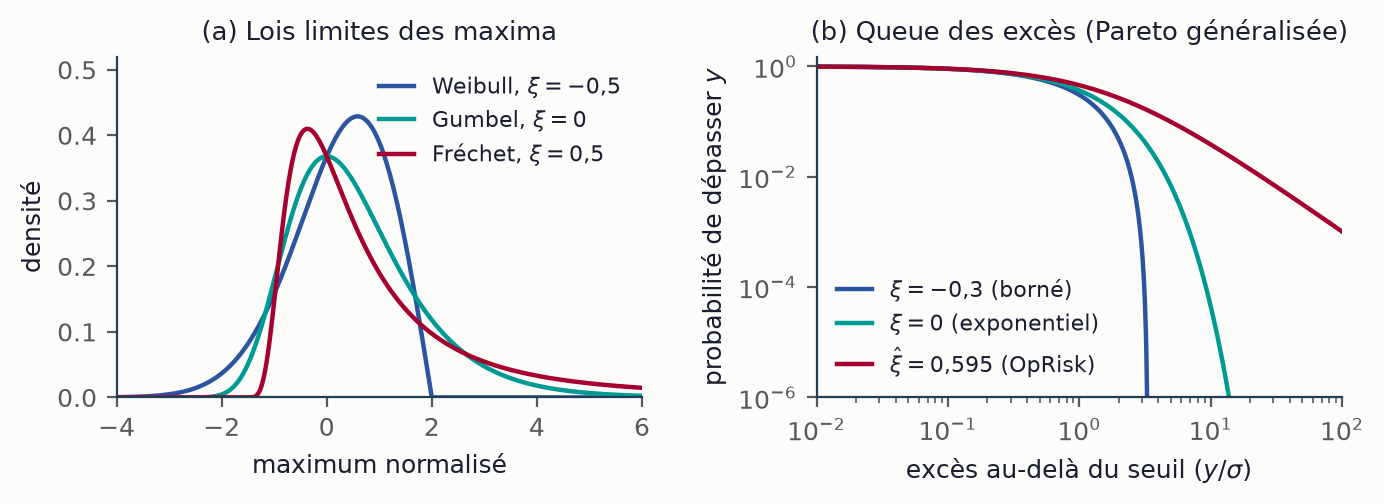
\includegraphics[width=0.95\textwidth]{GEV_domaines_attraction.png}
\caption{Domaines d'attraction des maxima et queue calibrée. (a) Densités des lois des valeurs
extrêmes généralisées de type Weibull ($\xi=-0{,}5$, support borné), Gumbel ($\xi=0$) et Fréchet
($\xi=0{,}5$, queue lourde), valeurs d'illustration. (b) Probabilité qu'un excès dépasse $y$ sous
une loi de Pareto généralisée d'échelle unité, en échelles logarithmiques. Les excès sont bornés
pour $\xi=-0{,}3$, et leur probabilité de dépassement décroît exponentiellement pour $\xi=0$, en
puissance pour l'indice calibré sur OpRisk, $\hat\xi=0{,}595$, qui relève du domaine de Fréchet.}
% SOURCES-SCRIPTS: 112
\label{fig:domaines-attraction}
\end{figure}

En notant $\zeta_u=\Prob(X>u)$, noté $p_u$ dans la suite, on dispose de formes fermées
classiques pour le quantile d'\emph{un} sinistre et sa moyenne de queue \citep{mcneil2015}. Ce
quantile n'est pas un besoin de capital, car celui-ci n'apparaît qu'après agrégation annuelle et
propagation dans la cascade.

\begin{proposition}[Quantile et moyenne de queue d'une sévérité GPD]\label{soc:prop:varestvar}
Sous le modèle POT, pour $\alpha$ tel que $\qsev_\alpha(X)>u$ et $\xi\in(0,1)$ :
\begin{align}
\qsev_\alpha(X) &= \boxed{\,u + \frac{\sigma}{\xi}\left[\left(\frac{1-\alpha}{\zeta_u}\right)^{-\xi}-1\right]\,},\label{soc:eq:var-gpd}\\[4pt]
\qbarsev_\alpha(X) = \E[X\mid X>\qsev_\alpha(X)] &= \boxed{\,\frac{\qsev_\alpha(X)}{1-\xi}+\frac{\sigma-\xi u}{1-\xi}\,}.\label{soc:eq:tvar-gpd}
\end{align}
Lorsque $\xi\ge 1$, l'espérance $\E[X]$ est infinie et $\qbarsev_\alpha$ n'est pas définie.
\end{proposition}

\noindent La calibration OpRisk ($u=20{,}03$, $\sigma=57{,}97$, $\xi=0{,}595$, $\zeta_u=0{,}151$)
donne par \eqref{soc:eq:var-gpd} un quantile de sévérité $\qsev_{99{,}5\%}(X)=663{,}0$~M\euro\ et
par \eqref{soc:eq:tvar-gpd} une moyenne de queue $\qbarsev_{99{,}5\%}(X)=1\,752{,}4$~M\euro. Ces
deux nombres décrivent un sinistre et ne se comparent jamais à un besoin de capital. Celui-ci est
$\VaR_{99{,}5\,\%}(L)$, quantile de la charge annuelle agrégée $L$, de l'ordre de plusieurs milliards
d'euros pour le périmètre financier étudié. Nous réservons $\VaR$ et $\TVaR$ à $L$,
$\qsev$ et $\qbarsev$ à $X$. À $\lambda\simeq21{,}6$ incidents enregistrés par an, l'approximation par perte unique associe au quantile annuel à $99{,}5\,\%$ un quantile
par sinistre de l'ordre de $99{,}98\,\%$. Les deux
échelles sont confrontées au \S\ref{sec:ancrage}.
% SOURCES-SCRIPTS: 67

Le vecteur d'attaque décrit l'entrée de l'incident : hameçonnage, exploitation de vulnérabilité
ou chaîne d'approvisionnement. Le pilier DORA désigne le contrôle qui a cédé.
Les parts $\pi_v$ des vecteurs répartissent la fréquence, sans appariement avec les piliers.
Le premier pilier touché suit les parts d'amorce du chapitre~\ref{chap:cascade} ; la cascade décrit la propagation qui suit.

\section{Loi de fréquence}

La fréquence de référence $\lambda_{ref}$ est lue sur le périmètre financier de la base PRC
($\lambda_{ref} = 341$ notifications/an). Nous la décomposons en sous-fréquences par vecteur
d'attaque, selon la structure de la base Hackmageddon :
% SOURCES-SCRIPTS: 62
\begin{equation}
\lambda_{ref} = \sum_{v} \lambda_v,
\qquad
\lambda_v = \lambda_{ref} \times \pi_v,
\end{equation}
où $\pi_v$ est la part du vecteur $v$ ($38{,}8\,\%$ hameçonnage, $33{,}8\,\%$ exploitation de
vulnérabilités, $15{,}8\,\%$ chaîne d'approvisionnement, $6{,}3\,\%$ identifiants compromis, $5{,}3\,\%$
autres). Un
défaut de conformité sur une exigence n'agit ainsi que sur la sous-fréquence du vecteur qu'elle
atténue. Les $341$ notifications américaines, sans seuil de matérialité, ne servent qu'à cette décomposition par vecteur. La base entière en compte $2\,150$ par an. L'entrée du
moteur est la fréquence conventionnelle des événements TIC collectés par OpRisk, $\lambda \simeq 21{,}6$ par an
pour le périmètre financier étudié, et tout niveau de capital du chapitre~\ref{chap:resultats}
repose sur elle.

Afin de tenir compte de la surdispersion ($\sigma^2/\mu > 1$), nous modélisons la fréquence agrégée
$\lambda_{S_x} = \lambda_{\text{C}}\sum_v \pi_v\, m_{v,S_x}$ d'un scénario $S_x$ par une loi binomiale
négative. Nous attribuons à l'état conforme la fréquence historique $\lambda_{\text{C}}\simeq 21{,}6$.
C'est une hypothèse, car aucune base n'observe l'état de conformité.
Nous posons $\phi = \sigma^2/\mu = 9{,}2$, constant d'un scénario à l'autre, et le paramètre
$r$ est recalculé :
\begin{equation}
r_{S_x} = \frac{\lambda_{S_x}}{\phi - 1},
\qquad
p_{S_x} = \frac{r_{S_x}}{r_{S_x} + \lambda_{S_x}}.
\end{equation}
La surdispersion en régime de forte dégradation n'est pas observée, faute
d'historique de crise DORA.

Pour un mélange de Poisson, l'indice de dispersion $1+\lambda/r$ croît avec la fréquence à $r$ fixé.
Le moteur maintient $\phi$ constant et recalcule $r$. L'indice est de $1{,}19$ sur les $14\,944$ cellules firme-année du
panel, de $2{,}24$ sur la série annuelle sectorielle détendancée (IC~$95\,\%$ $[1{,}24\,;5{,}18]$,
dix-huit points), et nous retenons $9{,}20$ dans le moteur.

Cette dernière valeur est un choix de prudence sur la queue de fréquence, pas une calibration. Il
en va de même de la charge systémique $a=0{,}60$ du mélange de la fréquence (supplément), qui dépasse la
borne haute de l'intervalle de la charge empirique $a=0{,}122$ (IC~$95\,\%$ $[0{,}054\,;0{,}223]$).
La charge $a$ est le coefficient du facteur dans le mélange lognormal $\exp(aY-a^2/2)$. Passer du Poisson à la
binomiale négative posée relève le besoin de capital du périmètre financier étudié de $+9\,\%$, la queue
restant déterminée au $99{,}5\,\%$ par la perte unique dominante.
% SOURCES-SCRIPTS: 47 08b 67 41

Le moteur tire indépendamment les comptes annuels selon cette loi binomiale négative.
Le facteur commun de conformité $\Theta$ intervient dans les probabilités des états C, PC et NC
(chapitre~\ref{chap:multietats}), auxquels correspondent les scénarios $S_0$, $S_1$ et $S_2$.
Les capitaux publiés sont calculés dans ces états discrets.

\section{Loi de sévérité}
\label{soc:sec:severite}

Chaque pilier touché reçoit une sévérité élémentaire : zéro avec probabilité $1-p_u$, ou $u+Y$, avec $Y$ de loi GPD.
Les pertes sous le seuil sont négligées. La perte d'un incident est la somme de ces sévérités,
hypothèse d'additivité non testée faute de coûts observés par pilier. La fréquence compte les événements avant ce tirage.

% SOURCES-SCRIPTS: 07 47 63 67

Sur la population OpRisk de fréquence et de descente d'échelle, les $10\,\%$ d'incidents les plus graves concentrent $92{,}3\,\%$ de la perte totale
(chapitre~\ref{chap:donnees}), ce qui conduit à représenter la queue par une GPD au-delà d'un seuil $u$
(\emph{peaks-over-threshold}). Au seuil du percentile~85 ($u = 20{,}0$~M\euro, 91 excès) :
\begin{equation}
\hat{\xi}_{\text{OpRisk}} = 0{,}595 \quad (\text{IC}_{90\%}=[0{,}30\,;\,0{,}83]),
\qquad
\hat{\sigma}_{\text{OpRisk}} = 58{,}0~\text{M\euro},
\qquad
\qsev_{99{,}5\%}(X) = 663~\text{M\euro}.
\end{equation}
L'intervalle bootstrap du quantile de sévérité, $[411\,;\,1037]$~M\euro, représente un facteur~2{,}5
entre les bornes, dû à la seule incertitude de paramètre. Nous plaçons le seuil là où l'indice de
forme quitte la zone $\xi \geq 1$, dans laquelle l'espérance n'existe pas, tout en gardant assez
d'excès pour l'estimation ($n = 91 > 30$). Cet argument ne tient qu'au voisinage du seuil, l'indice
décroissant sur toute la plage (\S\ref{soc:sec:validation}).

\section{Estimateur de Hill}

% SOURCES-SCRIPTS: 47 63 67

Au seuil retenu ($k=86$), l'estimateur de Hill \citep{Hill1975} atteint $1{,}32$ et dépasse de
$120{,}8\,\%$ le maximum de vraisemblance. Sur $2\,000$ échantillons simulés sous le modèle publié,
les six valeurs observées de Hill tombent dans l'intervalle simulé à $90\,\%$, si bien que l'écart
correspond à celui qu'un indice de $0{,}595$ produit en échantillon fini. De plus, Hill croît avec $k$ alors que
le balayage de seuil fait décroître $\hat\xi$, ce qui serait inversé si la queue valait $1{,}32$.
Sur la PRC, $\hat\xi = 1{,}03$ concerne un autre objet, puisque la sévérité y est une puissance du
nombre d'enregistrements (\S\ref{sec:oprisk}).

\section{Adéquation des lois}
\label{soc:sec:validation}

Pour la sévérité, les tracés quantile-quantile et probabilité-probabilité s'alignent sur la
diagonale, et la vie résiduelle moyenne est linéaire au-delà du seuil (figure~\ref{soc:fig:validation}).
L'estimation $\hat\xi$ est stable à $0{,}5\,\%$ près au voisinage du seuil retenu, jusqu'au
percentile $85$ des données courantes. Du percentile $85$ au percentile $95$, elle décroît de
$0{,}60$ à $0{,}38$ sur quatre seuils comptant chacun au moins trente excès, sans sortir de
l'intervalle à $90\,\%$ publié, $[0{,}30\,;0{,}83]$. Sous le seuil retenu, elle remonte jusqu'à
$0{,}98$ et sort de cet intervalle, ce qui traduit le biais de seuil attendu et interdit de
descendre plus bas.

Les tests par bootstrap paramétrique (91 excès) ne rejettent ni la famille GPD (Anderson-Darling $p=0{,}96$,
écart de Kolmogorov-Smirnov mesuré aux seuls points d'observation, $p=0{,}89$), ni le couple $(\hat\xi,\hat\sigma)$ publié, paramètres imposés
(Anderson-Darling $p=0{,}99$, Kolmogorov-Smirnov $p=0{,}89$). Mesurée par simulation, la couverture
réelle de l'intervalle à $90\,\%$ de $\xi$ est de $86\,\%$, donc l'intervalle est trop
étroit et l'élargir d'environ $10\,\%$ rétablirait le nominal. La sous-couverture concerne l'incertitude de l'estimation ; elle n'établit pas le signe d'un biais du capital. Le taux de dépassement et la dérive d'échelle font l'objet de diagnostics distincts (\S\ref{sec:pu-coherence} et \S\ref{soc:sec:backtest}).

Le test du rapport de vraisemblance rejette le Poisson au profit de la binomiale négative (statistique $130{,}5$, $p\approx 10^{-30}$ sur $14\,944$ cellules firme-année), bien que $\Var/\E=1{,}19$ reste proche de un. Ce $p$ traite les cellules comme indépendantes et ignore la dépendance par firme ; le rejet ne calibre pas non plus le facteur $9{,}2$ du moteur.

\begin{figure}[H]\centering
\figover{J3_validation_adequation.png}
\caption{Adéquation du socle. (a-b) Diagrammes quantile-quantile et probabilité-probabilité de la sévérité
contre la GPD ajustée. (c) vie résiduelle moyenne, linéaire au-delà de $u$. (d) stabilité
de $\hat\xi$ au seuil. (e) test d'Anderson-Darling, loi nulle par bootstrap
paramétrique et statistique observée ($p=0{,}96$). (f) adéquation de la fréquence :
la binomiale négative colle aux comptes firme-année, le Poisson rate la queue.}
% SOURCES-SCRIPTS: 47 93
\label{soc:fig:validation}
\end{figure}

Une règle de stabilité appliquée à dix percentiles candidats retient $19{,}87$~M\euro{} contre
$20{,}03$ publiés, avec un quantile identique. Ce seuil est également le mieux ajusté du balayage.
La règle la plus permissive descendrait à $12{,}88$~M\euro{} et donnerait un quantile de sévérité
supérieur de $16{,}0\,\%$.

Lorsqu'on retire chacun des $91$ excès à son tour, le quantile de sévérité balaie une étendue de
$111{,}7$~M\euro, qui représente $17{,}9\,\%$ de l'amplitude de l'intervalle publié, sans jamais en
sortir. Le plus gros excès, $1\,380$~M\euro, le déplace de $-15{,}8\,\%$. Sur le périmètre
calibré, le maximum équivaut à $3{,}7$ fois le quantile à $99\,\%$, contre $52{,}7$ sur la base
entière.

Retirer les trois plus grosses pertes ramène le quantile sous la borne basse.
En retirer cinq le fait passer de $657{,}2$ (quantile recompté, contre $662{,}78$ publié) à $327{,}3$~M\euro.
L'indice $\xi$ passe alors de $0{,}60$ à $0{,}22$.
Le quantile publié dépend donc de ces quelques pertes. Ces tests portent sur la forme des lois, non sur le niveau du capital.
% SOURCES-SCRIPTS: 106 41

\section{Backtest hors échantillon}
\label{soc:sec:backtest}

Pour chaque année d'origine, nous ajustons les deux lois sur les seules observations antérieures et
évaluons la prévision de l'année suivante, puis l'origine avance d'un an. La fenêtre va de $2004$ à $2025$
($539$ incidents, douze années notées), car avant $2004$ la base compte de un à neuf incidents par
an, et $2026$ n'en compte que cinq. Le seuil est ré-estimé sur chaque échantillon d'apprentissage
par la règle du percentile $85$.

Un intervalle de prévision à $90\,\%$ contient la réalisation $11$ années sur $12$ ($91{,}7\,\%$)
sous la binomiale négative et $9$ sur $12$ ($75{,}0\,\%$) sous le Poisson. Le log-score cumulé de la binomiale négative dépasse celui du Poisson de $3{,}054$ nats, gain dû à trois années. Douze années donnent trop peu de puissance : ce
résultat va dans le sens du choix de la binomiale négative sans le démontrer, et il ne teste pas
le facteur de surdispersion posé dans le moteur. Le test de Kolmogorov-Smirnov sur la probabilité intégrale
des excès ne rejette pas la GPD ($D=0{,}100$, $p=0{,}4087$), avec peu d'excès donc peu de
puissance. Le test de Kupiec rejette la couverture des quantiles de sévérité à $99\,\%$
($p=0{,}0078$) et à $99{,}5\,\%$ ($p=0{,}0140$), avec $8$ et $5$ dépassements pour $2{,}8$ et
$1{,}4$ attendus. L'échelle de la queue dérive de $4{,}00\,\%$ par an, dont la moitié
d'inflation monétaire. L'effet sur le quantile de sévérité est
d'au moins $+24{,}7\,\%$.

Sous la sévérité dérivée, le facteur entre états (rapport des capitaux non conforme sur conforme, chapitre~\ref{chap:resultats}) passe de
$3{,}344$ à $3{,}124$ ($-6{,}6\,\%$) et l'écart en euros bouge de $-1{,}9\,\%$, par compensation
entre forme et échelle. La charge annuelle agrégée est rejetée pour la même cause, sur les dernières
années notées seulement. L'indépendance entre fréquence et sévérité tient sur les excès. Ce
défaut d'échelle figure au registre des limites (\S\ref{sec:pu-coherence}), et nous ne corrigeons
pas la valeur publiée.
% SOURCES-SCRIPTS: 89 90 91 102

Détecter un doublement du taux de dépassement avec $80\,\%$ de puissance demanderait $1\,811$ années à $99{,}5\,\%$, $905$ à $99\,\%$ et $78$ à $90\,\%$. Douze années ne valident donc pas la queue du capital.
       % ex-5
% =====================================================================
% VERSION ENSAE, REDUCTION SFE (phase 3, 1er octobre 2026) : chapitre 5, cascade dirigee entre piliers.
% Copie a texte constant de chapitres/07_cascade_dirigee.tex.
% Ne changent que les titres et les renvois repares, listes dans
% reduction/phase3.md.
% Lu par main_ensae.tex seul : ne jamais le faire lire par main_institut.tex,
% qui garde chapitres/.
% =====================================================================

\chapter{Cascade dirigée entre piliers}
\label{chap:cascade}

La matrice d'influence dirigée $W$ décrit la propagation entre les cinq piliers.
Le cadre latent ci-dessous sert à définir cette influence ; le capital est calculé par une marche
auto-évitante (\S\ref{sec:formalisation}). Le seuil latent $K_j$ est apparié à un seuil
statistique de matérialité $u_j$, non à une valeur fixée par DORA.

\section{Modèle de Vasicek à un facteur}

Le modèle structurel de Merton-Vasicek associe à chaque entité une variable latente $X$, qui
mesure le stress. Nous l'utilisons sous la probabilité historique : aucun prix ni aucune valeur de
firme n'est calculé. Le modèle s'écrit
\begin{equation}
X_i \;=\; \sqrt{\rho}\;Y \;+\; \sqrt{1-\rho}\;\varepsilon_i, \qquad \Var(X_i)=1,
\end{equation}
où $Y\sim\mathcal N(0,1)$ est le facteur systémique commun, $\varepsilon_i\sim\mathcal N(0,1)$ le
choc idiosyncratique, et $\rho\in[0,1]$ la part du systémique, commune à toutes les entités.
L'incident survient lorsque le stress franchit un seuil, $D_i=\mathbf 1\{X_i\ge K_i\}$, avec dans
le modèle classique, seuil de défaut du crédit, $K_i=\Phi^{-1}(1-\mathrm{PD}_i)$.

Deux hypothèses de ce modèle ne s'appliquent pas au cyber sous DORA. La dépendance y est
symétrique, avec un $Y$ et un $\rho$ uniques, alors que la matrice posée à dire d'expert est
nettement asymétrique : la norme de l'écart entre la matrice et sa transposée vaut $81\,\%$ de celle de la matrice. Le seuil $\Phi^{-1}(\mathrm{PD})$ suppose de plus une PD stable et mesurable et
une valeur de firme sous-jacente, qui n'existent pas en cyber.

% SOURCES-SCRIPTS: 01 03

\section{Facteur systémique par pilier}

Nous indexons désormais par entité~$i$ et pilier~$j\in\{1,\dots,5\}$, et remplaçons le facteur
unique par un facteur systémique par pilier $Y_j$ et une sensibilité propre $\rho_{ij}$ :
\begin{equation}
X_{ij} \;=\; \sqrt{\rho_{ij}}\;Y_j \;+\; \sqrt{1-\rho_{ij}}\;\varepsilon_{ij}.
\end{equation}
Les $Y_j$ sont corrélés entre eux par une matrice $\Sigma_Y$, qui décrit les dépendances croisées
au niveau systémique. Elle prolonge les modèles latents gaussiens du crédit (copule des temps de défaut, \citet{Li2000}).

Les données étudiées ne permettent pas de calibrer un $\rho_{ij}$ par entité. La probabilité marginale de non-conformité reste
à $0{,}35$, quelle que soit cette sensibilité ; seule la co-variation des cellules partageant un facteur la renseigne.
Même avec $Y_j$ connu, détecter un écart de $0{,}10$ demande environ $813$ périodes indépendantes,
d'après une approximation locale de la puissance à $80\,\%$.

Sur une coupe unique, deux fois la divergence de Kullback-Leibler atteint $0{,}47$ pour l'alternative la plus éloignée, $\rho_{ij}=0{,}99$.
Cette moyenne du double log-rapport de vraisemblance ne se compare pas au seuil de $3{,}84$.
Au niveau du pilier, il faut de l'ordre de $474$ périodes à quatre entités, et de $81$ sur une population entière.
Dans ce cadre, l'information vient de la répétition dans le temps.

Une extension serait le compromis hiérarchique $\rho_{ij}=\rho_j+u_{ij}$. Sa variante
$\mathrm{logit}\,\rho_{ij}=\mathrm{logit}\,\rho_j+u_{ij}$ reste dans $[0\,;\,1]$ par construction,
alors que le terme additif en sort avec une probabilité de $1{,}40\,\%$ pour une dispersion de
$0{,}20$. Le modèle publié garde une sensibilité unique et n'utilise pas cette extension.
Au chapitre~\ref{chap:multietats}, le facteur est celui de l'entité : l'approximation locale donne environ $374$ entités observées une fois chacune.

% SOURCES-SCRIPTS: 107

\section{Propagation dirigée}
\label{sec:baremes}

La propagation repose sur un modèle qualitatif de cascade, qui note les chaînes d'effondrement
entre piliers à partir de trois barèmes posés par l'auteur à dire d'expert
(figure~\ref{fig:baremes}). Aucune de leurs valeurs n'est mesurée. Elles sont ancrées sur la
structure du règlement, et nous n'en défendons que l'ordre.
\begin{itemize}[leftmargin=*,itemsep=2pt]
\item $\mathrm{ROOT}_p$ est la propension du pilier $p$ à amorcer une chaîne. Elle vaut $1{,}00$
  pour la gouvernance, qui fonde les autres contrôles, $0{,}90$ pour les tiers, surface d'attaque
  externe, et $0{,}30$ pour le partage d'informations, rarement déclencheur. Dans le moteur, un
  incident naît sur le pilier $p$ avec une probabilité proportionnelle à $\mathrm{ROOT}_p$, soit
  des parts d'amorce de $30\,\%$ (P1, gouvernance), $27\,\%$ (P4, tiers), $18\,\%$ (P2), $15\,\%$
  (P3) et $9\,\%$ (P5, partage d'informations).
\item $\mathrm{TRANS}_{jk}$ est la force avec laquelle la défaillance du pilier $j$ entraîne celle
  du pilier $k$. Ses vingt entrées vont de $0{,}10$ à $0{,}80$ et sont asymétriques : la
  gouvernance entraîne la gestion des incidents à $0{,}80$, l'inverse ne vaut que $0{,}20$. Ce
  sont des forces d'entraînement et non des probabilités, si bien que les lignes ne somment pas à
  un. Normalisée par l'équation~\eqref{eq:norm}, $\mathrm{TRANS}$ devient la matrice de contagion
  $W$.
\item $\mathrm{GBASE}_p$ est le score de gravité (au sens de l'AMDEC) du pilier $p$ s'il cède seul,
  sans rapport avec le gain de propagation $g$. Sur cette échelle ordinale, il vaut $7$ pour les tiers, qui transmettent la contagion, $6$ pour la gouvernance, $4$ et
  $3$ pour la gestion des incidents et les tests, $1$ pour le partage d'informations, qui est
  volontaire.
\end{itemize}
Dans le modèle qualitatif, le score de vraisemblance d'une chaîne ordonnée est le produit de $\mathrm{ROOT}$
au pilier d'amorce et de $\mathrm{TRANS}$ le long de ses maillons. Sa gravité part du
$\mathrm{GBASE}$ le plus élevé et croît avec les autres piliers touchés et avec la force moyenne des
maillons. Sa criticité, notée de $1$ à $10$, est la moyenne géométrique des deux. C'est elle que
mesure la dépendance à l'ordre du \S\ref{sec:verif-proprietes}. Le moteur de capital n'emploie que
$\mathrm{ROOT}$ et $\mathrm{TRANS}$. La sévérité y suit la même loi pour tous les piliers : c'est
une hypothèse, aucune base n'observant la sévérité par pilier, et les tests du
\S\ref{sec:profilage-variables} montrent seulement un effet faible des catégories de la base.

\begin{figure}[H]\centering
\figover{Z_baremes_expert.png}
\caption{Les trois barèmes d'expert du modèle qualitatif. (a)~$\mathrm{ROOT}$, propension de
chaque pilier à amorcer une chaîne. (b)~$\mathrm{GBASE}$, gravité du pilier s'il cède seul.
(c)~$\mathrm{TRANS}$, force avec laquelle le pilier source entraîne le pilier cible, asymétrique.}
\label{fig:baremes}
\end{figure}

Dans tout le rapport,
\[
  \boxed{\;W_{jk}\;=\;\text{propension du pilier } j \text{ (source) à entraîner la
  défaillance du pilier } k \text{ (cible).}\;}
\]
La ligne $j$ décrit ce que $j$ émet, la colonne $k$ ce que $k$ reçoit, comme dans le graphe
d'arêtes vivantes (définition~\ref{def:cascade}). Dans $\mathrm{TRANS}$, P1 a la plus grande somme
de ligne ($2{,}6$) et une somme de colonne trois fois inférieure à celle de P2 : il émet fort et
reçoit peu, et $W$ en garde les proportions. Le stress de $j$ subit celui des autres piliers de la même entité, et somme donc les colonnes :
\begin{equation}
X_{ij} \;=\; \underbrace{\sum_{k\neq j} W_{kj}\,X_{ik}}_{\text{contagion dirigée, } k \to j}
   \;+\; \sqrt{\rho_{ij}}\,Y_j \;+\; \sqrt{1-\rho_{ij}}\,\varepsilon_{ij},
\end{equation}
d'où, en forme matricielle sur les cinq piliers, la forme réduite
$\mathbf X_i=(I-W^{\top})^{-1}(\text{systémique}+\text{idio})$. Cette forme suppose
$\rho(W)<1$, le rayon spectral étant invariant par transposition. Si
$W=0$, on retombe sur le modèle à facteur par pilier, puis, avec un facteur unique, sur le Vasicek
standard. Les trois modèles latents s'emboîtent strictement. La figure~\ref{fig:reseau-W} représente $W$.

% SOURCES-SCRIPTS: 29 113

\section{Normalisation de Leontief et stabilité}

La matrice d'expert TRANS ne peut pas servir telle quelle : $(I-W)^{-1}$ ne représente
une cascade que si la série $I+W+W^2+\cdots$ converge, ce qui équivaut à $\rho(W)<1$. Pour TRANS,
on a $\rho(\mathrm{TRANS})=1{,}461>1$, et $(I-\mathrm{TRANS})^{-1}$ contient 21 entrées négatives
sur 25, si bien qu'un choc positif produirait un stress négatif ailleurs.

% FIGURE FIXEE ICI EN [H], ET ELLE EST APPELEE UNE PAGE PLUS HAUT (\S de la propagation
% dirigee). En [htbp] a son point d'appel elle derivait jusqu'a cette page-ci et s'inserait au
% milieu de la phrase de Leontief, coupant l'inverse B=(I-A)^{-1} de sa somme. Elle ne peut pas
% tenir sous son paragraphe d'appel (191 pt disponibles pour 242 demandes) et la retrecir
% mettrait ses etiquettes sous 5 pt. Posee ici, elle ouvre la page et le paragraphe la suit
% entier. Ne pas la remettre en [htbp].
\begin{figure}[H]\centering
\figover{H1_reseau_W.png}
\caption{Structure dirigée de $W$ sur les cinq piliers (P1 émet fort et reçoit peu) et
propagation d'un choc sur un sous-réseau.}
\label{fig:reseau-W}
\end{figure}

Le correctif vient du modèle entrées-sorties de Leontief, dont l'inverse
$B=(I-A)^{-1}=\sum_{k\ge0}A^k$ n'explose jamais parce que $A$ est une matrice de parts. Ses
colonnes somment à moins de un, la différence étant la valeur ajoutée, strictement positive.
Nous appliquons la même règle en lisant la ligne $j$ de $W$ comme les parts du stress que $j$
\emph{émet} vers les autres piliers :
\begin{equation}
\label{eq:norm}
\boxed{\;W \;=\; g \cdot \frac{\mathrm{TRANS}}{\max_j \sum_k \mathrm{TRANS}_{jk}}\;,
\qquad g \in (0,\,1]\;}
\end{equation}
où $g$, le gain de propagation, est la somme de ligne maximale de $W$ (P1, somme de ligne de TRANS $2{,}6$).
Le paramètre $g$ est posé, non estimé (valeurs $0{,}45$, $0{,}68$ et $0{,}90$ au
chapitre~\ref{chap:multietats}). $W$ est positive et chaque ligne somme à
au plus $g$, donc par Perron-Frobenius
\begin{equation}
\rho(W)\;\le\;\max_j\sum_k W_{jk}\;\le\;g\;\le\;1,
\end{equation}
avec $\rho(W)<1$ pour $g<1$. Numériquement, $\rho(W)=0{,}562\,g$, ce qui garde $\rho(W)<1$ à la borne
$g=1$ : $(I-W)^{-1}$ existe sur tout le domaine admissible. La
division par un même scalaire pour toutes les lignes préserve l'hétérogénéité de ce que reçoit
chaque pilier.

% SOURCES-SCRIPTS: 03 66

\section{Processus de branchement}
\label{sec:branch}

Les données ne permettent pas d'estimer le modèle simultané sur latentes. Nous le remplaçons par un
processus de branchement multitype : un incident sur le pilier~$j$ engendre, à la période suivante,
un nombre aléatoire d'incidents sur les autres piliers. La matrice de génération suivante $M$ compte des incidents :
\begin{equation}
M_{jk}\;=\;\Phi(\text{base}_k+W_{jk})-\Phi(\text{base}_k),
\end{equation}
où $\Phi(\text{base}_k)$ est l'incidence de fond du pilier cible.
Le rayon spectral $\rho(W)$ détermine le système latent simultané, tandis que $R_0=\rho(M)$ détermine
le branchement auxiliaire, dont $R_0<1$ garantit l'extinction avec une descendance moyenne finie. La cascade du modèle, qui ne revient jamais sur un pilier touché, s'arrête de toute façon. Avec une incidence de fond de
$4{,}5\,\%$ et $g=0{,}9$, valeurs posées, on obtient $\rho(W)=0{,}506$ et $R_0=0{,}054$. Les seuils critiques,
$\rho(W)=1$ à $g=1{,}78$ et $R_0=1$ à $g=8{,}1$, sont hors du domaine admissible $g\le1$
(figure~\ref{fig:branchement-R0-rapport}). Le seuil critique de la forme simultanée est plus de quatre fois plus proche que celui du branchement.

La progéniture ($(I-M)^{-1}$ moins l'identité) compte les incidents moyens causés par un incident sur chaque pilier.
Elle vaut $0{,}109$ (P1), $0{,}069$ (P4), $0{,}058$ (P2), $0{,}054$ (P3)
et $0{,}026$ (P5). Elle reproduit le classement ROOT (Spearman $=1{,}00$) à $g=0{,}9$.
ROOT et TRANS venant du même expert, cet accord est un test de cohérence interne.
Il ne détermine pas les valeurs de ROOT, qui restent posées séparément.

\begin{figure}[H]\centering
\figover{K3_branchement_R0.png}
\caption{Stabilité de la cascade et progéniture. (a)~Sur le domaine admissible $g\le1$, les deux
rayons spectraux restent inférieurs à $1$ ; les seuils critiques ($\rho(W)=1$ à $g=1{,}78$ ;
$R_0=1$ à $g=8{,}1$) sont hors domaine. (b)~La progéniture $(I-M)^{-1}$ reproduit le classement
ROOT du jugement d'expert.}
% SOURCES-SCRIPTS: 03
\label{fig:branchement-R0-rapport}
\end{figure}

% SOURCES-SCRIPTS: 03 29

\section{Seuil $K_j$, substitut de $\Phi^{-1}(\mathrm{PD})$}

Le seuil statistique $u_j$ se définit dans l'espace des sévérités observables. Le seuil $K_j$ s'applique à la variable latente, sans unité. Nous apparions leurs
probabilités, en choisissant $K_j$ pour que l'événement latent $\{X_{ij}\ge K_j\}$ ait la même
probabilité que l'incident majeur observable $\{S_{ij}\ge u_j\}$ :
\begin{equation}
\label{eq:Kj}
\boxed{\;K_j\;=\;F_{\mathrm{latent}}^{-1}(1-p_j), \qquad p_j=\mathbb P(S_{ij}\ge u_j).\;}
\end{equation}
CreditMetrics \citep{jpmorgan1997} inverse également une fréquence cumulée observée. Le règlement ne fixe pas $p_j$ : le seuil reste celui, statistique, de la méthode POT. $F_{\mathrm{latent}}$ décrit un stress sans unité, à ne pas confondre avec la sévérité GPD, exprimée en euros.

Le biais sur $K_j$ vient de la sous-déclaration. Si $q(s)$ est la
probabilité qu'un incident de sévérité $s$ soit déclaré, alors
$\hat p_j^{\text{naïf}}/p_j=\mathbb E[q(S)\mid S\ge u_j]<1$. Il en résulte une sous-estimation de
$p_j$, qui conduit à surestimer $K_j$ et à sous-provisionner. Ce biais s'effondre toutefois lorsque
le seuil de matérialité monte dans la queue (biais sur $K_j$, sans unité, de $+0{,}369$ à $u=0{,}5$~M\euro{} contre
$+0{,}001$ à $u=40$~M\euro{}). Nous modélisons la sévérité au-dessus de ce seuil par la théorie des valeurs
extrêmes. Dans une simulation où l'indice de queue vrai est connu ($\xi=0{,}9$), le biais médian
sur le capital est de $-0{,}8\,\%$ pour cette méthode, d'écart interquartile $0{,}62$ rapporté au capital vrai, contre
$-63{,}9\,\%$ pour la lognormale.

% SOURCES-SCRIPTS: 04 02

\section{Calibration et faisabilité}
\label{sec:calib-cascade}

Les sources examinées n'identifient pas l'asymétrie de $W$. Une chronologie fiable ou la loi complète des ensembles touchés pourraient renseigner la direction,
sous des hypothèses sur la cascade et les amorces. Nous testons un probit dynamique, adapté au bruit gaussien du modèle générateur.
Un logit gonflerait les magnitudes d'un facteur $2{,}1$.

Sur un panel de $800$ entités et $60$ périodes simulé par ce modèle, le probit retrouve $W$ dans ses unités (corrélation $0{,}905$, pente $1{,}085$).
La corrélation tombe à $0{,}38$ avec $50$ entités. Ce contrôle ne valide aucune calibration sur données réelles.
Le probit ne peut pas être estimé sur les sources disponibles (chapitre~\ref{ch:identifiabilite}), d'où le capital en bornes du chapitre~\ref{chap:partielle}.

% SOURCES-SCRIPTS: 03 05

\section{Définitions et propriétés formelles}
\label{sec:formalisation}

On note
$P=\{1,\dots,5\}$ les piliers, $W\in[0,1]^{P\times P}$ la matrice de contagion avec
$W_{jj}=0$, et $s_{\max}=\max_j\sum_k \mathrm{TRANS}_{jk}$. Les démonstrations sont
rassemblées en annexe~\ref{ann:cascade}.

\begin{definition}[Cascade indépendante]
\label{def:cascade}
À chaque couple ordonné $(j,k)$, $j\neq k$, on associe une variable de Bernoulli
indépendante $B_{jk}\sim\mathcal B(W_{jk})$. Le \emph{graphe d'arêtes vivantes} $G$ possède
l'arc $j\to k$ si et seulement si $B_{jk}=1$. Pour un pilier d'amorce $a$, l'\emph{ensemble
atteint} est
\[
  S_a \;=\; \{a\}\cup\{k\in P : \text{il existe un chemin dirigé } a\rightsquigarrow k \text{ dans } G\}.
\]
C'est la cascade indépendante standard \citep{kempe2003}, une percolation de liens sur le graphe pondéré par $W$.
\end{definition}

\begin{proposition}[Forme réduite et descendance espérée]
\label{prop:reduite}
La somme, sur les marches dirigées de longueur $n$ de $a$ vers $k$, du produit des poids de
leurs arêtes vaut $(W^n)_{ak}$, et la série de ces termes est
\[
  \sum_{n\ge 0}(W^n)_{ak} \;=\; \bigl((I-W)^{-1}\bigr)_{ak},
\]
convergente si et seulement si $\rho(W)<1$. Un pilier atteint l'étant par au moins un chemin vivant
sans pilier répété, on a la majoration $\mathbb E\,|S_a|\le \bigl[(I-W)^{-1}\mathbf 1\bigr]_a$, et
l'écart mesure les marches qui répètent un pilier et les piliers atteints par plusieurs chemins.
\end{proposition}

\begin{proposition}[Sous-criticité par normalisation de Leontief]
\label{prop:leontief}
Sous la normalisation~\eqref{eq:norm}, $W=(g/s_{\max})\,\mathrm{TRANS}$, la matrice $W$ est
positive et chacune de ses lignes somme à au plus $g$ ; par conséquent
\[
  \rho(W)\;\le\;\max_j\sum_k W_{jk}\;\le\;g\;\le\;1 .
\]
Pour $g<1$, cette borne garantit $\rho(W)<1$, donc la convergence de $(I-W)^{-1}$ et la sous-criticité de l'enveloppe de branchement. La cascade finie sans réactivation s'arrête indépendamment de cette condition. À la borne $g=1$ du domaine, elle ne donne que $\rho(W)\le 1$ : la stabilité tient
alors par la valeur calculée de $\rho(W)$, strictement inférieure à $1$.
\end{proposition}

\begin{proposition}[Loi exacte de l'ensemble atteint]
\label{prop:loi}
Pour tout $A\subseteq P$ avec $a\in A$,
\[
  \mathbb P(S_a=A)\;=\;R(A)\,B(A),\qquad
  B(A)=\!\!\prod_{j\in A,\;k\notin A}\!\!(1-W_{jk}),
\]
où $B(A)$ est la probabilité qu'aucune arête ne fuie hors de $A$, et $R(A)$, la probabilité
que $a$ atteigne \emph{tout} $A$ par les seules arêtes internes, vérifie $R(\{a\})=1$ et
\[
  R(A)\;=\;1-\sum_{\substack{A'\subsetneq A\\ a\in A'}} R(A')\!\!\prod_{j\in A',\;k\in A\setminus A'}\!\!(1-W_{jk}).
\]
\end{proposition}

\noindent Les capitaux des chapitres~\ref{chap:multietats} et~\ref{chap:resultats} sont calculés avec la variante à un successeur par pas, la marche
auto-évitante. Depuis le pilier $j$, la cascade passe au pilier $k$ avec la probabilité $W_{jk}$, et
s'arrête sinon, ou dès qu'elle revient sur un pilier touché. Les deux constructions ont la même
matrice moyenne et le même nombre moyen de descendants directs, et leurs lois se calculent
sans approximation. Les bornes du chapitre~\ref{chap:partielle} emploient la cascade indépendante, la
seule définie pour les matrices admissibles dont une ligne somme à plus de un. Passer de la marche au branchement déplace le besoin de capital du secteur de $-4\,\%$. Pour la marche, la
croissance du capital en $g$ est vérifiée numériquement au \S\ref{sec:invariance-g}.

\begin{proposition}[Monotonie stochastique]
\label{prop:mono}
Si $W\le W'$ terme à terme, alors $S_a(W)$ est stochastiquement dominé par $S_a(W')$. Toute
fonctionnelle croissante de $S_a$, en particulier la perte agrégée et sa VaR, est donc
croissante en chaque entrée de $W$. En revanche une perturbation \emph{antisymétrique}
$A$ déplace $W_{jk}$ et $W_{kj}$ en sens opposés : le capital n'est pas monotone en $A_{jk}$,
ce qui justifie de balayer les sommets de l'ensemble admissible
(chapitre~\ref{chap:partielle}) sans revendiquer de bornes exactes.
\end{proposition}

\begin{proposition}[Dépendance à l'ordre]
\label{prop:ordre}
Soit la vraisemblance d'une chaîne ordonnée
\[
\ell(i_1,\dots,i_n)=\mathrm{ROOT}_{i_1}\prod_{k=1}^{n-1}\mathrm{TRANS}_{i_k i_{k+1}}.
\]
Sur les chaînes de deux piliers, $\ell$ est invariante par
permutation si et seulement si
\[
\mathrm{ROOT}_i\,\mathrm{TRANS}_{ij}=\mathrm{ROOT}_j\,\mathrm{TRANS}_{ji}
\]
pour tout couple $(i,j)$. Cette condition est nécessaire à l'invariance pour toute longueur. Le barème la viole pour la paire (P1, P2), dont les deux ordres reçoivent des criticités différentes (chapitre~\ref{ch:positionnement}). Un score ou une copule des seules indicatrices ne représente pas l'ordre d'atteinte.
\end{proposition}

\begin{proposition}[Ce que la co-occurrence voit de la direction]
\label{prop:nonid}
Soit la décomposition unique $W=S+A$, avec $S=\tfrac12(W+W^\top)$ et $A=\tfrac12(W-W^\top)$.
\emph{(i)} Sous une amorce uniforme, de probabilité $r$ pour chaque pilier, la probabilité qu'un
même sinistre touche à la fois $j$ et $k$ vaut
\[
  \sum_{a\in P} r\,\mathbb P\bigl(\{j,k\}\subseteq S_a\bigr)
  \;=\; r\,(W_{jk}+W_{kj})+O\bigl(\lVert W\rVert^2\bigr)
  \;=\; 2r\,S_{jk}+O\bigl(\lVert W\rVert^2\bigr) :
\]
au premier ordre, la co-occurrence ne dépend de $W$ que par $S$ ; $W$ et $W^\top$ y sont
indiscernables. \emph{(ii)} Au-delà du premier ordre, ou sous une amorce non uniforme, la loi de
l'ensemble atteint dépend en général de $A$. $W$ et $W^\top$ ne sont donc pas observationnellement
équivalents pour la loi complète des ensembles de piliers touchés. \emph{(iii)} En général,
$\mathrm{SCR}(W)\neq\mathrm{SCR}(W^\top)$.
\end{proposition}

% SOURCES-SCRIPTS: 32 61 29 98

\section{Vérification numérique des propriétés}
\label{sec:verif-proprietes}

% SOURCES-SCRIPTS: 32
Sur les $26$ sous-ensembles de taille au moins deux, $22$ changent de criticité selon l'ordre,
l'écart atteignant $6$ points sur une échelle de $10$, c'est-à-dire $60\,\%$ de l'échelle. Sur la
paire $\{P_1,P_2\}$, $\mathrm{TRANS}[1][2]=0{,}80$ et $\mathrm{TRANS}[2][1]=0{,}20$ donnent des
criticités de $8$ et $2$ pour le même ensemble. Ni une copule ni un score additif ne peuvent
reproduire cet objet (proposition~\ref{prop:ordre}). La
non-transitivité de la dominance entre piliers, testée sous trois formulations, ne se vérifie pas,
avec zéro violation sur $420$ triplets, une valeur propre minimale de $+0{,}405$ et zéro cycle.
Nous ne la revendiquons donc pas.

Avec le classeur actuel, on a $\rho(W)=0{,}506$. La majoration $\E\,|S_a|\le[(I-W)^{-1}\mathbf 1]_a$
tient sur les cinq amorces et sur $300$ matrices de l'ensemble admissible. L'écart entre la borne
et la valeur exacte, de $10{,}6\,\%$ (amorce P5) à $19{,}9\,\%$ (amorce P1), comprend les
contributions des marches avec répétitions et des chemins multiples vers un même pilier. Nous gardons le calcul exact (proposition~\ref{prop:loi}).

Sur les transitions annuelles OpRisk, le test de permutation de l'asymétrie ne rejette pas $A=0$
(asymétrie $119$ contre $128 \pm 27$, $z=-0{,}33$, aucune arête significative sur $18$). Pour le
périmètre financier étudié, aux paramètres de base, retourner la matrice déplace pourtant le capital de $3{,}6\,\%$
($295$~M\euro) et la perte moyenne de $7{,}9\,\%$, et le pilier à remédier en premier passe de P1 à
P4. Sur l'ensemble admissible, l'écart entre une matrice et sa transposée atteint $1\,173$~M\euro{}.

La loi complète des ensembles touchés distingue les deux matrices, puisque, à $g=0{,}90$, cascade seule et hors choc commun P4, un sinistre touche en
moyenne $1{,}931$ pilier sous $W$ et $1{,}746$ sous $W^\top$. La part des sinistres multi-piliers
passe de $62{,}31\,\%$ à $50{,}77\,\%$, et la probabilité que P2 et P5 cèdent ensemble de $0{,}127$
à $0{,}066$. Sous amorce uniforme, l'écart n'est plus que de $0{,}86\,\%$ lorsque $W$ est ramenée
au cinquantième de sa valeur. Les statistiques disponibles ne séparent pas les deux matrices, dont les capitaux diffèrent pourtant.

% SOURCES-SCRIPTS: 40 03 98
                  % ex-6
% =====================================================================
% VERSION ENSAE, REDUCTION SFE (phase 3, 1er octobre 2026) : chapitre 6, modelisation multi-etats de la conformite.
% Copie a texte constant de chapitres/11_conformite_multietats.tex.
% Ne changent que les titres et les renvois repares, listes dans
% reduction/phase3.md.
% Lu par main_ensae.tex seul : ne jamais le faire lire par main_institut.tex,
% qui garde chapitres/.
% =====================================================================

\chapter{Modélisation multi-états de la conformité}
\label{chap:multietats}


\section{Deux échelles de temps}

Le besoin de capital dépend de l'état de conformité de l'entité, qui est gradué et évolue dans le
temps. Nous le modélisons à deux échelles. La couche rapide est celle des incidents et de leur
cascade dans l'année, chiffrée par le moteur du chapitre~\ref{chap:cascade} conditionnellement à
une configuration de conformité. Un Vasicek multi-états y classe chaque pilier comme non
conforme (NC), partiellement conforme (PC) ou conforme (C). La couche lente est celle de la
gouvernance, où une chaîne de Markov fait progresser la conformité sur des mois et des années, et son
état sert de paramètre à la couche rapide.

La structure est celle d'un modèle de crédit à migration de rating (\S\ref{sec:couplage}). Nous
séparons les deux horloges afin d'empêcher qu'une tendance longue explique un enchaînement de
quelques heures. Le préprint de cascade climatique \citep{ccrn2026} distingue aussi
le temps calendaire du pas de propagation.

\section{Vasicek multi-états à seuils ordonnés}

Chaque pilier possède une capacité de conformité latente $C^\star\sim\mathcal N(0,1)$, que nous
décomposons à la Vasicek en un facteur systémique commun $\Theta$ et un choc idiosyncratique :
\begin{equation}
C^\star \;=\; \gamma\,\Theta \;+\; \sqrt{1-\gamma^2}\,\varepsilon, \qquad \gamma=0{,}68.
\end{equation}
Au lieu d'un unique seuil de défaut, nous en posons deux, ordonnés, qui découpent trois
états :
\begin{equation}
\text{NC si } C^\star\le K_{\text{bas}}, \quad
\text{PC si } K_{\text{bas}}<C^\star\le K_{\text{haut}}, \quad
\text{C si } C^\star>K_{\text{haut}}.
\end{equation}
La charge $\gamma$ et les probabilités d'état sont posées à partir de proxies externes
(annexe~B). Pour NC, PC et C, nous retenons $0{,}35$, $0{,}35$ et $0{,}30$, d'où $K_{\text{bas}}=\Phi^{-1}(p_{\text{NC}})$ et
$K_{\text{haut}}=\Phi^{-1}(p_{\text{NC}}+p_{\text{PC}})$. Sachant l'environnement $\Theta$, on
obtient
\begin{equation}
\mathbb P(\text{NC}\mid\Theta)=\Phi\!\Big(\tfrac{K_{\text{bas}}-\gamma\Theta}{\sqrt{1-\gamma^2}}\Big),
\qquad
\mathbb P(\text{C}\mid\Theta)=1-\Phi\!\Big(\tfrac{K_{\text{haut}}-\gamma\Theta}{\sqrt{1-\gamma^2}}\Big).
\end{equation}
Intégrée sur $\Theta$, la marginale redonne l'ancrage, tandis qu'en crise systémique la masse bascule
vers la non-conformité (figure~\ref{fig:multietats-rapport}).

\begin{figure}[H]\centering
\figover{S10_scr_multi_etats.png}
\caption{États de conformité et capital. (A)~Besoin de capital du périmètre financier étudié par état, en cumulant la fréquence seule,
puis la propagation, puis la détection, trois des canaux définis au
\S\ref{sec:quatre-canaux}. (B)~Probabilités d'état en régime normal et en crise systémique : la
masse bascule vers la non-conformité.}
% SOURCES-SCRIPTS: 16
\label{fig:multietats-rapport}
\end{figure}

% SOURCES-SCRIPTS: 63


\section{Quatre canaux de la conformité}
\label{sec:quatre-canaux}

L'état de conformité agit sur la cascade par quatre canaux, l'agrégation restant inchangée. Le
tableau donne la valeur de chacun aux deux états extrêmes, où tous les piliers partagent le même état
(\S\ref{sec:etat-par-pilier}).

\begin{center}\footnotesize
\renewcommand{\arraystretch}{1.2}
\begin{tabular}{@{}l l r r >{\raggedright\arraybackslash}p{4.6cm}@{}}
\toprule
\textbf{Canal} & \textbf{Paramètre} & \textbf{Conforme} & \textbf{Non conforme} & \textbf{Statut} \\
\midrule
Fréquence & $\lambda$, incidents enregistrés par an & $21{,}56$ & $53{,}62$ & multiplicateur posé \\
Propagation & $g$, gain de la normalisation & $0{,}45$ & $0{,}90$ & valeurs posées \\
Détection & $p_u$, dépassement par pilier touché & $0{,}128$ & $0{,}181$ & multiplicateurs $0{,}85$ et $1{,}20$ posés \\
Accumulation & probabilité de choc commun & $0$ & $0{,}68$ & borne haute posée, non identifiée \\
\bottomrule
\end{tabular}
\end{center}

Chacun des quatre est décrit ci-dessous.
\begin{enumerate}[leftmargin=1.5em,itemsep=2pt,topsep=2pt]
\item L'état module la \emph{fréquence} $\lambda$ des incidents amorcés par un multiplicateur de
  scénario, de $21{,}56$ incidents enregistrés par an à l'état conforme à $53{,}62$ à l'état non
  conforme.
\item Le gain de \emph{propagation} $g$ de la normalisation~\eqref{eq:norm} baisse de $0{,}90$ à
  $0{,}45$, car une entité plus conforme contient mieux la contagion. La propension du pilier $j$ à
  propager vaut $e_j=g(c_j)\,s_j/\max_k s_k$, où $s_j$ est la somme de la ligne $j$ de TRANS et
  $c_j$ l'état du pilier $j$.
\item La \emph{détection} agit sur $p_u$, le taux de dépassement, c'est-à-dire la probabilité
  qu'une sévérité élémentaire dépasse le seuil $u$ du chapitre~\ref{chap:socle}. Le moteur l'applique à chaque pilier touché, si bien que la probabilité de perte matérielle d'un incident est plus élevée et dépend aussi de la propagation. Le taux $p_u$ varie avec l'état parce qu'une entité conforme intercepte et remédie tôt, de sorte qu'une
  moindre fraction des piliers touchés atteint la sévérité matérielle. Nous multiplions $p_u$ par $0{,}85$
  à l'état conforme et par $1{,}20$ à l'état non conforme, deux valeurs posées.
\item L'\emph{accumulation par un prestataire commun} transforme, à l'état non conforme, un
  incident amorcé sur le pilier des tiers en choc commun. Ce choc touche chacun des autres piliers
  avec la probabilité $0{,}68$, borne haute posée égale à la charge $\gamma$, cette probabilité
  n'étant pas identifiée (\S\ref{sec:p4-accumulation}).
\end{enumerate}
Le résultat principal du chapitre~\ref{chap:resultats} fait varier les quatre canaux entre les deux états. Le multiplicateur de
fréquence se compose vecteur par vecteur selon $\lambda_{\text{NC}}=\lambda_{\text{C}}\sum_v \pi_v\,m_v$, où $\pi_v$ est la
part du vecteur $v$ dans le recensement Hackmageddon (\S\ref{sec:hackmageddon}) et $m_v$ le centre
d'une fourchette de multiplicateur propre au scénario non conforme.

\begin{center}\footnotesize
\renewcommand{\arraystretch}{1.2}
\begin{tabular}{@{}l r c r r >{\raggedright\arraybackslash}p{5.2cm}@{}}
\toprule
\textbf{Vecteur} & \textbf{Part $\pi_v$} & \textbf{Fourchette} & \textbf{Centre} & \textbf{$\pi_v\,m_v$} & \textbf{Effet publié qui ancre la fourchette} \\
\midrule
Hameçonnage & $0{,}388$ & $[1{,}8\,;3{,}0]$ & $2{,}40$ & $0{,}9312$ & réduction du risque par la formation (Ponemon/IBM) \\
Exploitation de vulnérabilité & $0{,}338$ & $[2{,}0\,;2{,}6]$ & $2{,}30$ & $0{,}7774$ & écart de conversion en intrusion entre exploitation et hameçonnage (ENISA) \\
Chaîne d'approvisionnement & $0{,}158$ & $[1{,}9\,;2{,}6]$ & $2{,}25$ & $0{,}3555$ & surcoût et progression des brèches d'origine tierce (IBM, SecurityScorecard) \\
Identifiants compromis & $0{,}063$ & $[3{,}0\,;8{,}0]$ & $5{,}50$ & $0{,}3465$ & réduction de compromission par l'authentification forte (Microsoft Research) \\
Autres & $0{,}053$ & $[1{,}3\,;1{,}6]$ & $1{,}45$ & $0{,}0769$ & aucune source dédiée \\
\midrule
\multicolumn{4}{@{}l}{Multiplicateur agrégé, état non conforme} & $2{,}4875$ & $21{,}56\times 2{,}4875 = 53{,}62$ incidents par an \\
\bottomrule
\end{tabular}
\end{center}

\noindent Ce multiplicateur est posé, non calibré : les parts sont une citation externe, et
chaque fourchette traduit un effet publié en multiplicateur prudent. Aux bornes des fourchettes, il
va de $1{,}933$ à $3{,}042$, ce qui donne une fréquence non conforme de $41{,}7$ à $65{,}6$ incidents
par an. Le vecteur des identifiants, avec $6{,}3\,\%$ des incidents, représente $13{,}9\,\%$ du
multiplicateur.

% SOURCES-SCRIPTS: 67 99 43


\section{Valeurs posées de \texorpdfstring{$g$}{g} et invariance de l'ordre}
\label{sec:invariance-g}

Les trois valeurs du gain de propagation,
\[
  g = 0{,}45 \ \text{(conforme)}, \qquad 0{,}68 \ \text{(partiellement conforme)},
  \qquad 0{,}90 \ \text{(non conforme)},
\]
sont posées : aucune donnée ne donne la relation état $\to g$, les états DORA n'étant pas publiés.
Pour une entité de $15\,000$~M\euro{} de provisions (\S\ref{sec:ancrage}), le besoin passe de $116$ à $169$~M\euro{}
quand $g$ passe de $0{,}45$ à $0{,}90$. Le montant de $169$ reste une extrapolation d'ordre de grandeur.

La croissance du capital en $g$ est contrôlée numériquement.
Sur une grille de vingt points, à nombres aléatoires communs, aucun pas n'est décroissant, pour le
capital comme pour la perte moyenne, à l'échelle d'entité comme du secteur. Les applications testées respectant $g_C < g_{PC} < g_{NC}$ donnent $\mathrm{SCR}_C < \mathrm{SCR}_{PC} < \mathrm{SCR}_{NC}$. La grille ne démontre pas cette propriété pour toute valeur de $g$. L'existence et le sens de l'écart sont
ainsi vérifiés numériquement sur ces vingt points et sur les cinq applications du tableau, et seule
son amplitude est un scénario.

\begin{center}\small
\renewcommand{\arraystretch}{1.25}
\begin{tabular}{@{}l r r r r r@{}}
\toprule
\textbf{Application état $\to g$} & \textbf{Conf.} & \textbf{Part.} & \textbf{Non conf.} &
\textbf{Écart} & \textbf{Ordre} \\
 & M\euro & M\euro & M\euro & & \\
\midrule
étroite $(0{,}70 / 0{,}80 / 0{,}90)$ & $145{,}5$ & $156{,}5$ & $169{,}0$ & $+16{,}2\,\%$ & oui \\
\textbf{retenue} $(0{,}45 / 0{,}68 / 0{,}90)$ & $\mathbf{116{,}4}$ & $\mathbf{143{,}2}$ &
$\mathbf{169{,}0}$ & $\mathbf{+45{,}2\,\%}$ & oui \\
large $(0{,}20 / 0{,}55 / 0{,}90)$ & $94{,}4$ & $126{,}4$ & $169{,}0$ & $+79{,}1\,\%$ & oui \\
conformité faible $(0{,}45 / 0{,}55 / 0{,}65)$ & $116{,}4$ & $126{,}4$ & $139{,}2$ &
$+19{,}5\,\%$ & oui \\
très étroite $(0{,}85 / 0{,}875 / 0{,}90)$ & $162{,}6$ & $166{,}7$ & $169{,}0$ & $+3{,}9\,\%$ &
oui \\
\midrule
\emph{repère forfaitaire de Formule Standard} & $450$ & $450$ & $450$ & $0\,\%$ & \emph{plat} \\
\bottomrule
\end{tabular}
\end{center}

\vspace{2pt}
\noindent Avec un déplacement de $0{,}05$ sur $g$, l'écart est de $+3{,}9\,\%$, le forfait restant plat. L'hypothèse qui demeure est qualitative, $g_C < g_{NC}$, et signifie que se conformer à
DORA réduit la propagation entre piliers. L'élasticité d'arc du capital au gain est de $0{,}41$ sur
$g \in [0{,}20\,;0{,}95]$, et un écart de $10\,\%$ ne demande qu'une baisse de $g$ de $0{,}90$ à
$0{,}75$. Nous présentons donc l'écart entre états comme un scénario sur l'écart entre les valeurs de $g$ au
chapitre~\ref{chap:resultats}.
% SOURCES-SCRIPTS: 66 67

\section{État de conformité par pilier}
\label{sec:etat-par-pilier}

Chaque pilier reçoit sa propre latente $C^\star_j$, les cinq étant corrélées par le facteur commun
$\Theta$. Un pilier non conforme propage alors plus et détecte moins que ses voisins conformes. Les
canaux deviennent $\lambda_j$, $g_j$ et $p_{u,j}$, indexés par pilier. Le moteur redonne
la version globale lorsque tous les piliers partagent un état, et basculer un pilier à la
fois permet de décomposer le surcoût de non-conformité par pilier (chapitre~\ref{chap:resultats}).

\subsection{Dépendance entre états}
\label{sec:dependance-etats}

% SOURCES-SCRIPTS: 69 77 94

La conformité aux piliers~1 et~2 pourrait aider à satisfaire les exigences du pilier~3 si les contrôles se recouvrent. Cette hypothèse n'est pas observée. Les
cinq latentes partagent le facteur systémique avec une charge de $0{,}68$, soit une corrélation de
$0{,}462$ entre deux piliers quelconques. Cette dépendance est identique pour toutes les paires.

Ajouter un surcroît
de corrélation $\delta$ aux deux seules paires concernées, à marges fixées, est admissible jusqu'à
$\delta = 0{,}38$. Sur ce balayage, la probabilité que les cinq piliers soient non conformes passe
de $0{,}068$ à $0{,}088$ et celle qu'aucun ne soit non conforme de $0{,}291$ à $0{,}330$. Ce diagnostic est binaire : son état C regroupe PC et C, contrairement au modèle à trois états. Le capital
espéré, pour le périmètre financier étudié, ne varie que de $2$~M\euro, soit $0{,}02\,\%$.

Dans les $32$ configurations, la fréquence, la propagation et la détection varient, tandis que l'accumulation reste fixe.
Les capitaux vont de $6\,015$ à $17\,009$~M\euro. Une forme additive en indicateurs de pilier les approche avec $R^2 = 0{,}9945$.
Les contributions sont de $3\,524$ (P1), $2\,863$ (P4),
$2\,022$ (P2), $1\,577$ (P3) et $897$~M\euro{} (P5) au-dessus d'un socle tous conformes.
L'espérance d'une fonction additive ne dépend que des marges, donc l'invariance tient pour toute
structure de dépendance à marges fixées. Cette quasi-additivité est le même fait que la faible
interaction entre piliers, de signe non résolu (section sur la décomposition par pilier,
chapitre~\ref{chap:resultats}).

L'argument concerne une
espérance et ne se transpose ni au quantile de la loi de perte mélangée, où l'invariance est
seulement non détectée, ni au quantile de la loi des configurations, où l'effet est de quelques pour
cent.

\section{Chaîne de Markov et séjours de type phase}

% SOURCES-SCRIPTS: 17 77 08b

À l'échelle lente, l'état suit une chaîne de Markov à temps continu
$\text{NC}\to\text{PC}\to\text{C}$, dont l'état conforme est absorbant dans le cas de base. Le
retour vers un état moins conforme est traité en sensibilité. Nous posons des séjours d'Erlang à $k=2$ phases,
de durée moyenne $1{,}5$ an par état transitoire. Le taux par phase est $\mu_0=k/(1{,}5\ \text{an})$ dans le régime de référence.
Cette loi réduit les séjours très courts sans imposer de durée minimale. On développe chaque
macro-état transitoire en $k$ phases, et l'on résout le générateur $Q$ par exponentielle de matrice :
\begin{equation}
\big(\mathbb P(\text{NC},t),\mathbb P(\text{PC},t),\mathbb P(\text{C},t)\big)
\;=\; \text{(sommes de phases de)}\;\; v_0\,\exp(Qt),
\end{equation}
où $v_0$ place les masses $0{,}35$, $0{,}35$ et $0{,}30$ en première phase de NC, PC et en C. Cette distribution pondère les besoins de capital par état :
\begin{equation}
\overline{\mathrm{SCR}}(t)\;=\;\sum_{e\in\{\text{NC,PC,C}\}}\mathbb P(e,t)\,\mathrm{SCR}_e .
\end{equation}
Il s'agit d'une moyenne de quantiles, qui diffère du quantile à $99{,}5\,\%$ de la loi mélangée,
dont la queue vient des composantes les plus lourdes. Sur les $32$ configurations, le quantile du mélange dépasse la moyenne des quantiles de $9{,}3\,\%$. La trajectoire se lit donc comme l'espérance du
besoin de capital sous l'incertitude d'état.

% SOURCES-SCRIPTS: 08b 77

\section{Couplage systémique et analogie de crédit}
\label{sec:couplage}

Le même facteur $\Theta$ agit sur les deux couches. Un environnement dégradé, où $\Theta<0$,
ralentit la remédiation par des taux de transition $\mu(\Theta)=\mu_0\,e^{\beta_{\text{rem}}\Theta}$
et durcit la cascade par $\mathrm{SCR}_e(\Theta)=\mathrm{SCR}_e\,e^{-\beta_{\text{casc}}\Theta}$,
deux formes exponentielles posées, avec $\beta_{\text{rem}}=0{,}35$ et $\beta_{\text{casc}}=0{,}1$. Elles introduisent la corrélation entre conformité et
sinistralité, et la dispersion de $\Theta$
engendre la bande d'incertitude de la trajectoire. La chaîne de Markov joue le rôle de la migration
d'un rating de conformité, et le Vasicek multi-états celui du défaut conditionnel au rating. Les
résultats chiffrés figurent au chapitre~\ref{chap:resultats}.

% SOURCES-SCRIPTS: 63 17
               % ex-7
% =====================================================================
% VERSION ENSAE, REDUCTION SFE (phase 3, 1er octobre 2026) : chapitre 7, identifiabilite de la direction de contagion.
% Copie a texte constant de chapitres/09_identifiabilite.tex.
% Ne changent que les titres et les renvois repares, listes dans
% reduction/phase3.md.
% Lu par main_ensae.tex seul : ne jamais le faire lire par main_institut.tex,
% qui garde chapitres/.
% =====================================================================

% ---------------------------------------------------------------------
% STATUT : RÉÉCRIT (juillet 2026). La thèse passe de « W n'est pas
%          identifiable » à une frontière en TROIS NIVEAUX : structure
%          corroborée, direction par paire non établie, amplitude jamais
%          identifiable. Sources : scripts 40, 53, 55, 56.
% LABELS À PRÉSERVER : ch:identifiabilite (cité par 8 chapitres),
%          fig:reversibilite (cité par 12b).
% ---------------------------------------------------------------------
\chapter{Identifiabilité de la direction de contagion}
\label{ch:identifiabilite}

Pour deux piliers $j$ et $k$, nous appelons \emph{direction} le sens de la contagion, de $j$ vers $k$
($W_{jk}$) ou de $k$ vers $j$ ($W_{kj}$). Les sources publiques examinées n'offrent aucun panel homogène des défaillances par pilier. Les comptages agrégés qu'elles permettent n'en donnent pas le sens, alors que la loi
complète des piliers touchés par incident la contient (proposition~\ref{prop:nonid}). Un corpus de
rapports d'incidents officiels en corrobore l'ordre sans en fixer les coefficients, d'où une
frontière en trois niveaux et un capital lu en bornes.

\section{Conditions d'identification de $W$}

Le coefficient $W_{jk}$ mesure la propension d'une défaillance du pilier $j$ à entraîner une
défaillance du pilier $k$, la ligne émettant et la colonne recevant (chapitre~\ref{chap:cascade}).
Pour l'identifier, il faut observer des co-occurrences de défaillances de piliers dans une même
entité. Pour distinguer $W_{jk}$ de $W_{kj}$, on peut utiliser une chronologie fiable ou la loi complète des ensembles de piliers touchés,
sous des hypothèses sur la cascade et les amorces. Il faut aussi une taxonomie par domaine de contrôle ; le classement par vecteur d'attaque ne suffit pas.

Aucune des trois sources agrégées que nous avons examinées ne réunit ces conditions. La première n'a
pas la taxonomie, la deuxième n'a pas le pas de temps, et la troisième prévoit les deux dans son
schéma sans les renseigner.

\section{Trois sources agrégées}

La première source, la chronologie américaine des fuites de données, est volumineuse
($74\,783$ incidents, $25\,009$ organisations) mais manque de taxonomie et de volume informatif. La
catégorie non déterminée (\texttt{UNKN}) représente en effet 52,7\,\% des incidents. La date de
survenance n'est exploitable que dans 49,6\,\% des cas, de façon non aléatoire selon le type
d'incident, et ordonner par date de déclaration mesurerait le délai de détection, pas la contagion.
Restreinte aux types informatifs et aux trimestres consécutifs, la base ne donne que 71 transitions
$j(t\!-\!1)\to k(t)$, c'est-à-dire $3{,}6$ observations par cellule hors diagonale, et 34 dans le
secteur financier.

La deuxième, SAS OpRisk, offre 4\,329 transitions annuelles entre 7 catégories de risque, environ 103
par cellule, mais son pas de temps annuel est trop grossier pour saisir une antériorité. On note $M$
la matrice des transitions observées, $M_{jk}$ comptant les passages $j(t-1)\to k(t)$, et l'on pose
\begin{equation}
  T(M) \;=\; \tfrac{1}{2}\,\lVert M - M^{\top}\rVert_1
        \;=\; \tfrac{1}{2}\sum_{j\neq k}\bigl|M_{jk}-M_{kj}\bigr| ,
  \label{eq:asymetrie}
\end{equation}
nulle si et seulement si $M$ est symétrique. Nous permutons les années à l'intérieur de chaque firme
afin de détruire l'antériorité en conservant la co-occurrence. Si $\mu_0$ et $\sigma_0$ désignent la
moyenne et l'écart-type de $T$ sur ces permutations, l'écart réduit
\begin{equation}
  z \;=\; \frac{T(M)-\mu_0}{\sigma_0}
  \label{eq:placebo-z}
\end{equation}
s'établit à $z = -0{,}33$, avec $T(M) = 119$ contre $\mu_0 \pm \sigma_0 = 128 \pm 27$. Aucune des 18
paires suffisamment peuplées n'est significative à 5\,\%, avant ou après correction de Bonferroni. Le
test du temps inversé, qui compare $M$ à la matrice de la chronologie renversée, est dégénéré sur un
comptage, cette matrice étant $M^\top$, et seul le placebo par permutation est donc utilisable.

La troisième, la VERIS Community Database, compte $10\,591$ incidents, dont $980$ en secteur
financier (NAICS~52). Son schéma prévoit les deux objets manquants, à savoir un champ
\texttt{control\_failure} qui nomme le domaine de contrôle défaillant, et une chronologie en quatre
étapes. Le champ est renseigné dans $13$ incidents ($0{,}12\,\%$), dont un seul en secteur financier,
et la chronologie est datée sur au moins deux étapes dans $126$ incidents ($1{,}19\,\%$), sur au moins
trois dans $10$. L'intersection des deux conditions compte $1$ incident, extérieur au secteur
financier. La spécification existe donc mais n'est pas remplie, et il s'agit d'en rendre le
remplissage obligatoire (section~\ref{ch:livrable}).

% SOURCES-SCRIPTS: 05 57

% SOURCES-SCRIPTS: 28 40 64 110

% SOURCES-SCRIPTS: 40 64

\section{Direction de contagion et réversibilité}

Nous nous plaçons sous la mesure physique : il n'y a ni prix ni mesure risque-neutre, et aucun test de
martingalité au sens des générateurs de scénarios n'est conduit. Sous l'hypothèse que les sauts entre
piliers forment une chaîne de Markov stationnaire, la théorie des processus réversibles explique que
la co-occurrence ne dise rien de la direction. Toute matrice se décompose de façon unique en
$W=S+A$, partie symétrique $S=(W+W^\top)/2$ et antisymétrique $A=(W-W^\top)/2$, orthogonales au sens
de Frobenius. Cette décomposition euclidienne de $W$ ne s'identifie pas à celle d'une chaîne de Markov de loi stationnaire non uniforme. Pour une chaîne auxiliaire de noyau $P$ et de loi stationnaire $\pi$ strictement positive, le noyau adjoint est $\tilde P_{jk} = \pi_k P_{kj}/\pi_j$ et $S_\pi=\tfrac12(P+\tilde
P)$ est réversible. Avec $A_\pi=(P-\tilde P)/2$, le courant vaut $J_{jk}=2\pi_j(A_\pi)_{jk}$, nul à l'équilibre détaillé. La forme de Dirichlet s'écrit
\begin{equation}
  \mathcal{E}(f,f) \;=\; \tfrac12\sum_{j,k}\pi_j P_{jk}\,(f_k-f_j)^2
                  \;=\; \tfrac12\sum_{j,k}\pi_j (S_\pi)_{jk}\,(f_k-f_j)^2 ,
  \label{eq:dirichlet}
\end{equation}
la partie antisymétrique pondérée s'annulant par paires. L'énergie de fluctuation $\mathcal{E}(f,f)$ est donc aveugle à la
direction (figure~\ref{fig:reversibilite-rapport}). L'invariance par renversement du temps n'interdit pas de détecter l'intensité d'une irréversibilité : $T$ en est un exemple, puisqu'elle est elle-même invariante par transposition. Elle ne donne pas le signe du courant. Le placebo ne détecte pas d'asymétrie au pas annuel ; ce non-rejet n'établit pas la réversibilité.

Deux limites bornent cette lecture. La matrice
$W$ n'est pas un générateur de Markov au sens strict, et l'énoncé ne s'étend pas à la loi complète
des ensembles de piliers touchés, qui dépend de la direction (proposition~\ref{prop:nonid}). La
frontière tient aux statistiques que fournissent les sources.

\begin{figure}[H]\centering
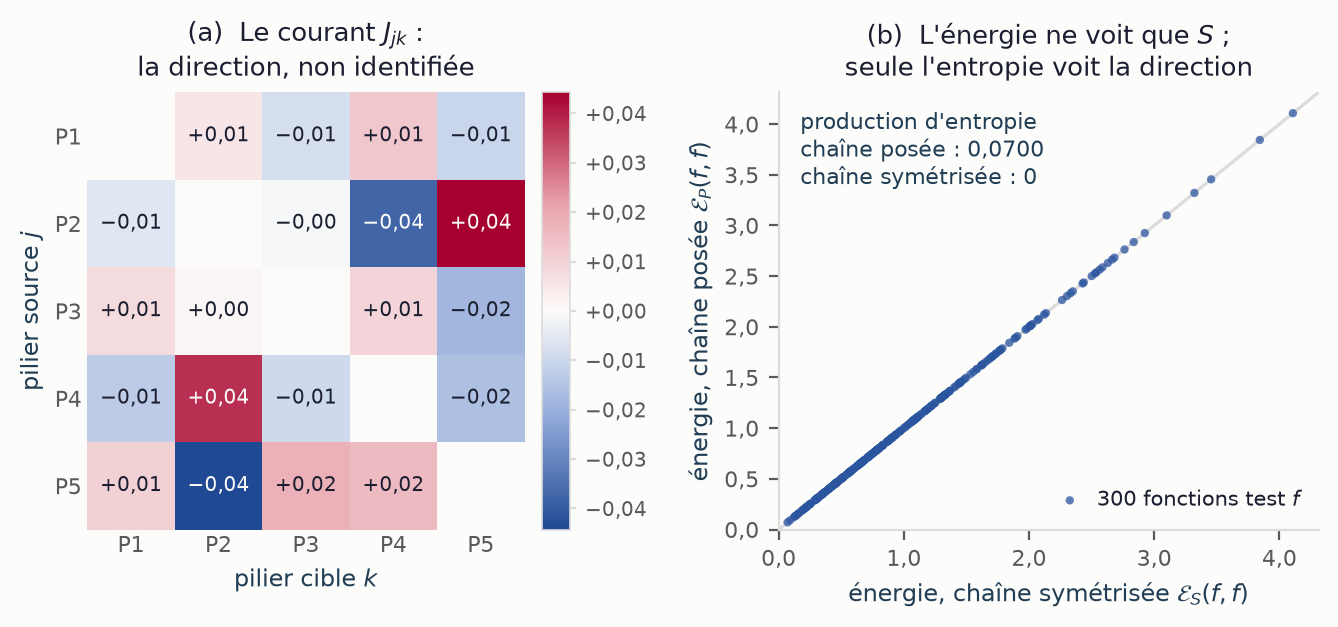
\includegraphics[width=0.95\textwidth]{Z11_reversibilite_martingale.png}
\caption{Direction et réversibilité. (a)~Le courant $J_{jk}=\pi_jP_{jk}-\pi_kP_{kj}$ est non nul, donc
le modèle a une direction. (b)~Pour trois cents fonctions test tirées au hasard, l'énergie de
fluctuation est la même pour la chaîne posée et pour sa symétrisée. Seule la production d'entropie,
nulle pour une chaîne réversible, distingue les deux chaînes.}
\label{fig:reversibilite-rapport}
\end{figure}
% SOURCES-SCRIPTS: 40

\section{Expérience naturelle du choc MOVEit}

En mai 2023, l'exploitation de masse de la faille du logiciel de transfert MOVEit frappe en même
temps des centaines d'organisations. Si la contagion dirigée existe, ce choc exogène, daté et rattaché
au pilier~4, doit élever dans les mois suivants, chez les organisations touchées, le risque de
défaillances relevant d'autres piliers. Une différence de différences sur
188 organisations financières touchées, contre un groupe de contrôle apparié et sur des fenêtres de
$180$~jours, donne $+1{,}17$ jour de déclaration d'incident par organisation (IC bootstrap $[+1{,}07\,;+1{,}27]$).

Calé sur une fausse date un an plus tôt, le même dispositif donne $+1{,}11$. L'effet est donc
compatible avec une régression vers la moyenne du groupe de contrôle sélectionné, et l'effet net de $+0{,}06$ est
indiscernable de zéro. La cible resterait de toute façon non attribuable, car la source classe les
incidents par vecteur d'attaque, avec $32\,\%$ de non déterminés.

% SOURCES-SCRIPTS: 62 35

\section{Corpus de rapports post-incident}
\label{sec:postmortems}

Un rapport post-incident officiel reconstitue la séquence des défaillances de contrôle, ce
qu'aucune base agrégée ne fait. Nous codons sept rapports (Cyber Safety Review Board, FCA et PRA,
GAO, SEC, OCC), dont deux sur des entités financières régulées, en transitions dirigées $j \to k$
telles que le rapport les décrit. L'unité de codage est le couple (incident, paire de piliers).

Sur $17$ transitions, l'asymétrie est de $17$, contre $8{,}4 \pm 2{,}2$ sous un placebo par
permutation, d'où $z=+3{,}93$ ($p=0{,}0004$), là où le pas annuel d'OpRisk donnait $z=-0{,}33$.
Toutes les transitions vont dans le sens dominant de leur paire. P1, la gouvernance, n'est jamais une
cible ($9$ sorties, $0$ entrée) et P2, la gestion des incidents, n'a aucune sortie ($0$ sortie,
$7$ entrées), structure que le classeur qualitatif (la matrice $W$ posée à dire d'expert) posait par jugement.

Le placebo teste la cohérence du codage, mais pas l'exogénéité de la direction. Une enquête
officielle, mandatée pour déterminer une cause racine, conclut en effet souvent à une défaillance de
gouvernance, si bien que P1 peut ressortir comme source par convention d'écriture. S'y ajoutent un
codeur unique, des sources en partie secondaires et un échantillon d'incidents notoires. Le corpus
corrobore donc la structure sans la calibrer, et le coût du biais est borné au
\S\ref{sec:biais-narration}. Une mesure de fiabilité par second codeur en aveugle reste en attente.

Les trois relectures de praticiens reçues ne distinguent pas un ordre de propagation d'une cause
commune, ce qui corrobore la frontière mais pas la matrice. Les deux dernières contestent le sens
unique de deux arcs sans déplacer le capital publié (supplément, \S\ref{sec:relecture-praticien}).
% SOURCES-SCRIPTS: 53

\section{Corpus étendu et matrice ordonnée}
\label{sec:corpus-etendu}

Nous ajoutons les trois rapports d'enquête publique sur CrowdStrike Falcon 2024, Log4Shell
2021--2022 et Raphaels Bank 2015. Le corpus compte alors $22$ transitions et le signal se renforce, y
compris lorsque l'on se restreint aux sources primaires ou à la perspective de l'entité.

\begin{center}\small
\renewcommand{\arraystretch}{1.25}
\begin{tabular}{@{}l r r r r@{}}
\toprule
\textbf{Périmètre} & \textbf{Rapports} & \textbf{Transitions} & \textbf{Asym.\ / nul} & $z$ \\
\midrule
Corpus initial (chapitre, ci-dessus) & $7$ & $17$ & $17$ / $8{,}4\pm2{,}2$ & $+3{,}93$ \\
\textbf{Corpus étendu} & $10$ & $22$ & $22$ / $9{,}5\pm2{,}4$ & $\mathbf{+5{,}12}$ \\
Sources \emph{primaires} seules & $7$ & $18$ & $18$ / $8{,}2\pm2{,}4$ & $+4{,}08$ \\
Perspective \emph{entité} seule & $6$ & $16$ & $16$ / $8{,}0\pm2{,}2$ & $+3{,}62$ \\
\bottomrule
\end{tabular}
\end{center}

\vspace{2pt}
\noindent Chaque incident déclare aussi l'ensemble des piliers défaillants, y compris ceux qui n'ont
rien entraîné. On en tire le dénominateur manquant et la matrice ordonnée complète :
\begin{equation}
\begin{gathered}
  p_{jk} \;=\; \Prob(\text{le rapport documente } j\to k \mid \text{le pilier } j \text{ a cédé}),
  \\
  p_{jk}\mid\text{données} \;\sim\; \mathrm{Beta}\bigl(1+m_{jk},\;1+N_j-m_{jk}\bigr),
\end{gathered}
  \label{eq:pjk}
\end{equation}
où $N_j$ compte les incidents où $j$ a cédé et $m_{jk}$ ceux où le rapport documente $j\to k$. Sur les
vingt liens ordonnés, douze ont un intervalle de crédibilité à $90\,\%$ situé sous $0{,}5$ et aucun au-dessus, si bien
que les transitions documentées y sont rares sans identifier les propagations fortes. Les liens les plus élevés,
$P_3\to P_2$ ($0{,}77$, intervalle $[0{,}48\,;0{,}95]$) et $P_1\to P_4$ ($0{,}68$, $[0{,}40\,;0{,}89]$),
recouvrent encore $0{,}5$.

Les douze liens faibles comprennent les quatre sorties de $P_2$ et trois des quatre entrées de $P_1$,
l'arc $P_5 \to P_1$ n'étant pas classé faible. La corrélation avec le classeur d'expert n'est pas
significative ($\rho=+0{,}08$ sur la matrice, $+0{,}31$ sur sa partie antisymétrique, $p=0{,}19$).
Si l'on ajoute au dénominateur des défaillances non propagées, le niveau moyen de $p_{jk}$ tombe de
$0{,}27$ à $0{,}07$, mais la part de direction $\lVert A\rVert/\lVert W\rVert$ reste à $60\,\%$.
Ce postérieur porte sur la documentation des transitions dans le corpus sélectionné ; l'absence de mention ne prouve pas l'absence de propagation. Le corpus suggère un ordre, sans en fixer l'intensité.
% SOURCES-SCRIPTS: 59

\section{Biais de narration}
\label{sec:biais-narration}

Onze des vingt-deux transitions codées partent de $P_1$, ce qu'une convention de cause racine pourrait
produire. Nous chiffrons ce biais par une loi nulle exacte, obtenue par convolution, et par une borne
adverse sur les $2^{11}$ sous-ensembles d'arêtes partant de $P_1$. Un jackknife montre que le signal
ne tient pas à un rapport isolé.

\begin{center}\small
\renewcommand{\arraystretch}{1.25}
\begin{tabular}{@{}l l l@{}}
\toprule
\textbf{Hypothèse sur les $11$ arêtes de $P_1$} & \textbf{Reste} & $p$ \textbf{exacte} \\
\midrule
Aucune (corpus tel qu'il est codé) & $22$ transitions & $1{,}5\cdot10^{-5}$ \\
$4$ arêtes \emph{retournées}, pire configuration & $22$ transitions & $\mathbf{0{,}084}$ \\
Les $11$ arêtes \emph{retirées} & $11$ transitions & $0{,}0039$ \\
Les $7$ \emph{rapports} concernés retirés & $3$ transitions & $0{,}50$ \\
\bottomrule
\end{tabular}
\end{center}

\vspace{2pt}
\noindent Il faudrait que la convention narrative ait inversé quatre des onze arêtes, dans
l'agencement le plus défavorable, pour perdre la significativité. Retirer tout le rôle de la
gouvernance, la moitié du corpus, ne suffit pas, car la direction subsiste dans les chaînes
$P_3\to P_2$ et $P_4\to P_2$, où $P_1$ ne figure pas. Retirer les sept rapports entiers écarte aussi
des chaînes que le biais ne concerne pas.

En capital, nous dégradons l'émission de $P_1$ par $W_{1k}\to(1-a)\,W_{1k}$ et recalculons la bande
à chaque degré. Le besoin de capital de l'entité notionnelle ($15\,000$~M\euro{} de provisions) passe de $169{,}0$ à
$127{,}1$~M\euro{} lorsque $P_1$ devient muette ($-24{,}8\,\%$) ; le $169{,}0$ est une extrapolation d'ordre de grandeur. Ce déplacement de $41{,}9$~M\euro{} représente
$0{,}81$ fois la largeur de la bande d'identification, $51{,}7$~M\euro, de sorte qu'admettre
l'objection dans toute son ampleur coûte moins que l'ignorance directionnelle déjà publiée. Le pilier
à remédier en premier passe toutefois de $P_1$ à $P_4$ dès $a = 0{,}50$. L'écart entre états de
conformité descend de $+45{,}2\,\%$ à $a=0$ à $+29{,}1\,\%$ à $a=1$ sans s'annuler, car la
conformité agit par $g$ sur toutes les arêtes.

% SOURCES-SCRIPTS: 54
% SOURCES-SCRIPTS: 64 65

\section{Formalisation bayésienne}
\label{sec:bayes}

Nous exploitons le même matériau dans un cadre bayésien, en posant un lien, que la donnée ne permet pas de vérifier, entre la fréquence d'une chaîne dans les rapports et le sens de la propagation. Pour chaque paire
$\{lo,hi\}$ de piliers, on note $\theta$ la probabilité qu'une chaîne documentée aille de $lo$ vers $hi$,
reliée au coefficient antisymétrique par
\[
  A_{lo,hi} \;=\; S_{lo,hi}\,(2\theta - 1),
\]
bijection croissante de $[0,1]$ sur l'intervalle admissible $[-S_{lo,hi},+S_{lo,hi}]$ du
chapitre~\ref{chap:partielle}. Avec $n_{lo}$ chaînes de $lo$ vers $hi$ et $n_{hi}$ dans l'autre sens,
\begin{equation}
  \begin{gathered}
  \theta \sim \mathrm{Beta}(\alpha_0,\beta_0),
  \qquad
  n_{lo}\mid\theta \sim \mathcal{B}\mathrm{in}(n_{lo}+n_{hi},\,\theta)
  \\
  \Longrightarrow\qquad
  \theta \mid \text{données} \;\sim\; \mathrm{Beta}\bigl(\alpha_0+n_{lo},\;\beta_0+n_{hi}\bigr).
  \end{gathered}
  \label{eq:posterieur-beta}
\end{equation}
Les quatre paires que le corpus ne documente pas gardent sous $\mathrm{Beta}(1,1)$ un $\theta$
uniforme, donc un coefficient qui couvre tout l'intervalle admissible. Le postérieur reproduit
l'identification partielle sans la poser. Le capital devient une loi, dont l'intervalle de
crédibilité à $90\,\%$ est $81\,\%$ plus resserré que les bornes de pire cas
(bornes du chapitre~\ref{chap:partielle}). Sous un prior sceptique, la médiane bouge à peine, mais seules deux des six
paires documentées ont un intervalle de crédibilité à $90\,\%$ qui exclut $\theta=1/2$. Nous retenons les bornes et publions l'intervalle à titre informatif.
% SOURCES-SCRIPTS: 56

\section{Frontière d'identification}

\begin{center}\small
\renewcommand{\arraystretch}{1.3}
\begin{tabular}{@{}p{3.2cm} p{7.4cm} p{4.2cm}@{}}
\toprule
\textbf{Objet} & \textbf{Ce que la donnée établit} & \textbf{Posture retenue} \\
\midrule
\textbf{Structure} \newline (P1 amont, P2 aval) &
$17$ transitions sur le corpus initial et $22$ sur le corpus étendu, aucune à contre-sens,
$z=+3{,}9$ puis $+5{,}1$ ; accord de la structure avec le classeur d'expert, non des coefficients ($\rho=+0{,}08$) ; codeur unique &
\textbf{revendiquée}, avec son confondant déclaré \\
\textbf{Direction} \newline paire par paire &
$2$ paires sur $6$ seulement ont un intervalle de crédibilité concluant &
\textbf{non revendiquée} ; les bornes restent \\
\textbf{Amplitude} \newline des coefficients &
aucune information ; même les dix sens connus, une bande de $656$~M\euro{} subsisterait &
\textbf{non identifiable} par cette voie \\
\bottomrule
\end{tabular}
\end{center}

\vspace{4pt}
\noindent Nous revendiquons donc un ordre partiel entre piliers, qui, combiné aux barèmes et aux scénarios retenus, contribue au classement et à l'ordre de remédiation. La donnée fixe par
ailleurs la fréquence marginale d'entrée, l'accumulation par cause commune et l'indice de queue de la
sévérité, et ce qu'elle ne fixe pas se lit en bande. La spécification du registre qui identifierait $W$ et
la valeur en capital de cette information font l'objet de la section~\ref{ch:livrable}.

% SOURCES-SCRIPTS: 55 59 64
          % ex-8
% =====================================================================
% VERSION ENSAE, REDUCTION SFE : chapitre 8, identification partielle et bornes de capital.
% Phase 3 : copie a texte constant de chapitres/10_identification_partielle.tex.
% Phase 4 (1er octobre 2026) : reecrit et condense ; formules, tableaux, figures, renvois,
% citation et nombres conserves. Le texte d'origine reste dans chapitres/ (version Institut)
% et dans l'historique Git.
% Lu par main_ensae.tex seul : ne jamais le faire lire par main_institut.tex,
% qui garde chapitres/.
% Scripts : 30 (bornes), 31 (comparaison des regimes), 33 (relatif/absolu), 34, 61, 67.
% =====================================================================
\chapter{Identification partielle et bornes de capital}
\label{chap:partielle}

La direction de la contagion n'étant pas identifiable (chapitre~\ref{ch:identifiabilite}), on peut
poser $W$ à dire d'expert et publier un besoin de capital ponctuel, ou caractériser l'ensemble des $W$
compatibles avec les contraintes posées et publier des extrema numériques. Nous suivons la seconde voie et la comparons à la
première. Les montants de ce chapitre valent pour le périmètre financier étudié, avec la
sévérité OpRisk, à titre illustratif.

\section{Modèle en couches}

Le socle, indépendant de $W$, regroupe la fréquence d'entrée surdispersée, l'accumulation par cause
commune et la sévérité GPD. Sans contagion ($W = 0$), le besoin de capital est de $5\,275$~M\euro{} dans le calage
de référence (sévérité OpRisk, fréquence de l'état conforme, gain de propagation $g=0{,}90$). Le préprint de cascade climatique \citep{ccrn2026} retire aussi la propagation dans une ablation, comme à $W=0$,
pour mesurer l'apport de la structure.

Toute matrice se décompose de façon unique en
\[
  W \;=\; S + A, \qquad S = \tfrac{1}{2}(W + W^{\top}), \qquad A = \tfrac{1}{2}(W - W^{\top}) .
\]
Ici $A_{jk}>0$ signifie que la contagion va plutôt de $j$ vers $k$, et $A_{jk}<0$ de $k$ vers $j$. Des
données de co-occurrence identifieraient $S$ au premier ordre sous amorce uniforme et faible intensité, mais pas $A$, la direction
(proposition~\ref{prop:nonid}). Faute d'un tel panel, nous posons $S$ à partir du barème d'expert
(chapitre~\ref{chap:cascade}) et ne faisons varier que $A$ : les bornes qui suivent sont donc
conditionnelles à cette partie symétrique posée. Nous définissons l'ensemble admissible par
\[
  \mathcal{W}(t) \;=\; \bigl\{\, S + A \;:\; A^{\top} = -A, \;\; |A_{jk}| \leq t\,S_{jk},
  \;\; \rho(S+A) < 1 \,\bigr\},
\]
où la contrainte $|A_{jk}| \leq S_{jk}$ découle des conditions de positivité $W_{jk}\geq 0$ et
$W_{kj}\geq 0$. Le paramètre $t\in[0,1]$ mesure ce que la donnée ignore de la direction, l'ignorance
totale $t=1$ correspondant aux sources publiques actuelles. Pour chacune des $10$ paires de piliers,
$A_{jk}/S_{jk}$ varie donc entre $-t$ et $t$ : les contraintes de signe définissent un pavé, intersecté avec la contrainte spectrale. Ses $2^{10} = 1\,024$ sommets fixent chaque paire à un extrême ; leur admissibilité est contrôlée avant évaluation.

% SOURCES-SCRIPTS: 31 30

\section{Capital sur l'ensemble admissible}

Nous appelons ici « bornes numériques » le minimum et le maximum calculés aux sommets admissibles, notés $V(1)$. Il ne s'agit pas de bornes globales démontrées sur $\mathcal W(1)$. À $t=1$, on obtient
\[
  \left[\min_{W\in V(1)}\widehat{\mathrm{SCR}}(W),\max_{W\in V(1)}\widehat{\mathrm{SCR}}(W)\right] \;=\; [\,6\,858 \;;\; 8\,697\,]~\text{M\euro{}} ,
\]
avec un facteur $1{,}27$ entre les deux bouts. La contagion ajoute entre $+30\,\%$ et
$+65\,\%$ au socle. Le point d'expert, $8\,110$~M\euro{}, n'est qu'un point de cet ensemble
(figure~\ref{fig:pave-sommets}).

\begin{figure}[H]
  \centering
  \figover{Z_pave_sommets.png}
  \caption{Le pavé admissible et le capital qu'il donne. (a)~Coupe sur deux des dix paires :
$A_{jk}/S_{jk}$ va de $-1$, tout de $k$ vers $j$, à $+1$, tout de $j$ vers $k$. (b)~Capital aux
$1\,024$ sommets et aux $3\,000$ points intérieurs, à $t = 1$ : aucun point intérieur ne sort des bornes.}
  \label{fig:pave-sommets}
\end{figure}

Les sommets ne bornent le capital que si les extrêmes y sont atteints, ce que rien ne garantit
\emph{a priori}. Augmenter $A_{jk}$ élève $W_{jk}$ mais abaisse $W_{kj}$, si bien que la
réponse n'est pas monotone en $A_{jk}$. Les $3\,000$ points intérieurs tirés uniformément restent tous
dans les bornes, en VaR comme en perte moyenne. Cette propriété reste vérifiée
numériquement, mais non démontrée. Ces extrema numériques sont des quantiles de $40\,000$ années
simulées, au bruit non mesuré. À indice de queue élevé, la VaR est peu sensible à la structure de
cascade, la queue annuelle étant dominée par une perte unique. La perte moyenne, bornée
dans $[849\,;1\,100]$~M\euro{} et moins bruitée, et l'ordre de remédiation en rendent mieux compte.

Ramener l'ignorance de $t=1$ à $t=0{,}5$, c'est-à-dire borner l'asymétrie à la moitié de la
co-occurrence, réduirait la largeur des bornes de $1\,839$ à $695$~M\euro{}, soit $-62\,\%$. Ce scénario donne l'ordre de grandeur de ce que le reporting de la section~\ref{ch:livrable} permettrait de gagner, sans le garantir.

% SOURCES-SCRIPTS: 30 61

\section{Comparaison d'une matrice posée et de l'identification partielle}

\begin{center}\footnotesize
\renewcommand{\arraystretch}{1.3}
\begin{tabular}{@{}p{4.1cm} p{4.5cm} p{5.6cm}@{}}
\toprule
 & \textbf{Régime A : on pose $W$} & \textbf{Régime B : modèle en couches} \\
\midrule
Sortie sur le capital & un point, $8\,110$~M\euro{} & socle $5\,275$ + bande $[6\,858\,;8\,697]$ \\
Part indépendante de la direction & aucune, tout repose sur le classeur & $79\,\%$ (socle $61\,\%$, plancher commun aux sommets $18\,\%$), à $S$ posé \\
Panel biaisé & déplace le besoin de capital de $777$~M\euro{} & la bande ne bouge pas si $S$ reste fixé \\
Priorité de remédiation & P1, sans marge d'erreur & tête P1/P4, ordre interne ouvert \\
Si aucun expert ne répond & plus de matrice complète & exploration conditionnelle au $S$ d'expert maintenu \\
\bottomrule
\end{tabular}
\end{center}

\vspace{2pt}
\noindent Faire varier la direction posée à dire d'expert, depuis un panel qui confirmerait le classeur
jusqu'à un panel qui dirait l'inverse au bord du pavé admissible, déplace le besoin de capital du
régime~A de $777$~M\euro{}, soit $10\,\%$. La priorité bascule alors entre trois piliers, sans signal
pour l'utilisateur. La
bande du régime~B ne bouge pas. Sur l'ensemble admissible, P5 n'arrive jamais en tête, P3 dans moins
de $10\,\%$ des cas, et P1 ($45\,\%$) et P4 ($36\,\%$) concentrent $81\,\%$ des matrices testées. Un panel d'experts servirait donc à départager
P1 et P4 et à resserrer la bande ; le questionnaire diffusé est resté sans réponse.

% SOURCES-SCRIPTS: 31

\section{Niveaux et rapports de capital}

\begin{center}\footnotesize
\renewcommand{\arraystretch}{1.25}
\begin{tabular}{@{}p{4.3cm} r r r r@{}}
\toprule
\textbf{Calibration} & \textbf{socle} & \textbf{bornes} &
\textbf{haute/socle} & \textbf{\% indépendant de la direction} \\
\midrule
Référence (OpRisk)   & $5\,275$  & $[6\,858\,;8\,697]$   & $1{,}65$ & $78{,}9\,\%$ \\
Sévérité PRC         & $239$     & $[336\,;424]$         & $1{,}77$ & $79{,}2\,\%$ \\
Fréquence $\times 3$ & $11\,709$ & $[14\,353\,;17\,405]$ & $1{,}49$ & $82{,}5\,\%$ \\
\bottomrule
\end{tabular}
\end{center}

\vspace{2pt}
\noindent La borne haute explorée varie d'un facteur $41$ entre les calibrations PRC et fréquence triplée ; il ne s'agit pas d'un rapport uniforme de tous les niveaux de capital. Les
rapports varient d'au plus $33\,\%$ de leur valeur moyenne, et l'ordre de remédiation place les mêmes
deux piliers, P1 et P4, en tête dans les trois calibrations.

Le rapport le moins stable est la largeur de bande rapportée au socle, qui varie de $32{,}9\,\%$ de sa valeur moyenne et
diminue lorsque la fréquence augmente, la queue annuelle étant alors moins dominée par une perte
unique. Ces rapports et le classement des piliers résistent au changement de source (figure~\ref{fig:partielle}).
% SOURCES-SCRIPTS: 33

\section{Échelle de repli sur la direction}
\label{sec:echelle-u}

On peut écrire la direction par l'excès de propagation propre à la source,
$\operatorname{logit}p_{ij}=\operatorname{logit}p_j+u_{ij}$ ($p_j$ mesure l'attractivité de la cible
$j$), puis limiter $u$ par paliers (crans), de $u$ libre au cran nul où $u=0$. Une direction de rang $1$ (une seule valeur singulière de $u$, figure~\ref{fig:echelle-repli}b) capte $74\,\%$ de la
variance de la direction posée et resserre les bornes de $25\,\%$, au prix d'une
hypothèse de structure. Au cran
nul, P1 et P4 deviennent indiscernables (gains de remédiation $1\,051$ contre $1\,052$~M\euro{}),
alors que $353$~M\euro{} les séparent avec la direction du classeur. C'est donc la direction qui
départage les deux piliers prioritaires.

\begin{figure}[H]\centering
\figover{Z5_echelle_repli.png}
\caption{Échelle de repli sur la direction. (a)~Les bornes du capital se resserrent quand la
direction descend d'un cran : $u$ libre, rang~$1$, classeur, puis cran nul ($u=0$). (b)~Valeurs
singulières de la direction posée : le rang~$1$ en capte l'essentiel. (c)~Gains de remédiation par
pilier avec la direction du classeur et au cran nul.}
% SOURCES-SCRIPTS: 34
\label{fig:echelle-repli}
\end{figure}

\begin{figure}[H]
  \centering
  \figover{Z_identification_partielle.png}
  \caption{Identification partielle de la contagion dirigée. (a)~Les bornes se resserrent quand
l'ignorance directionnelle $t$ diminue. (b)~Le prior d'expert dans des bornes indépendantes du
choix de direction, conditionnelles à la partie symétrique posée. (c)~Priorité de remédiation (regret maximal). (d)~Dominance des
piliers sur l'ensemble admissible : P5 n'arrive jamais en tête, et P1 et P4 concentrent $81\,\%$ des
matrices testées.}
  \label{fig:partielle}
\end{figure}
% SOURCES-SCRIPTS: 30 67

% SOURCES-SCRIPTS: 34

Les capitaux des chapitres~\ref{chap:multietats} et~\ref{chap:resultats} reposent sur la marche auto-évitante ; les extrema ci-dessus, sur la cascade indépendante. Les deux ne se comparent pas directement.
 % ex-9
% =====================================================================
% VERSION ENSAE, REDUCTION SFE (phase 3, 1er octobre 2026) : chapitre 9, resultats.
% Copie a texte constant de chapitres/12_resultats.tex.
% Ne changent que les titres et les renvois repares, listes dans
% reduction/phase3.md.
% Lu par main_ensae.tex seul : ne jamais le faire lire par main_institut.tex,
% qui garde chapitres/.
% =====================================================================

\chapter{Résultats}
\label{chap:resultats}
\label{part:resultats}

Les capitaux valent pour le périmètre financier étudié, non pour un assureur, et pour le
risque opérationnel d'origine informatique, sur deux périmètres de sévérité :
OpRisk, à queue lourde ($\hat\xi=0{,}595$), et PRC, plafonnée à $40$~M\euro{} par sévérité élémentaire ($\hat\xi=1{,}03$).
La variance de la sévérité étant infinie, nous donnons aussi la médiane et l'intervalle à $90\,\%$ du
bootstrap. Le niveau varie d'un facteur $41$ selon la loi de sévérité
et la fréquence (chapitre~\ref{chap:partielle}). Les rapports au socle (borne haute, largeur de bande)
varient d'au plus $33\,\%$ de leur valeur moyenne, et les deux piliers les plus coûteux restent P1 et
P4. Nous interprétons donc les écarts, non les niveaux.

À trois canaux (lecture~C), l'état conforme vaut $5\,932$~M\euro{} et à quatre canaux $6\,049$, soit
plus que le socle sans contagion du chapitre~\ref{chap:partielle}, $5\,275$~M\euro, parce qu'il
conserve une contagion.
% SOURCES-SCRIPTS: 65 66 12 16 63

\section{SCR par état de conformité}

Le besoin de capital croît de façon monotone de l'état conforme à l'état non conforme. Le
tableau~\ref{tab:scretat} donne trois lectures emboîtées : la lecture~A ne retient que la
fréquence, la lecture~B ajoute la propagation de la cascade, la lecture~C le canal de détection.

\begin{table}[htbp]\centering\small
\renewcommand{\arraystretch}{1.25}
\begin{tabular}{@{}l ccc c ccc@{}}
\toprule
& \multicolumn{3}{c}{\textbf{OpRisk} (M\euro)} & & \multicolumn{3}{c}{\textbf{PRC} (M\euro)} \\
\cmidrule(lr){2-4}\cmidrule(lr){6-8}
État & A & B & C & & A & B & C \\
\midrule
Conforme               & 8301  & 6664  & 5932  & & 2589 & 1903 & 1642 \\
Partiellement conforme & 11059 & 9625  & 9625  & & 3653 & 3118 & 3118 \\
Non conforme           & 15074 & 15074 & 16595 & & 5520 & 5520 & 6577 \\
\bottomrule
\end{tabular}
\caption{SCR par état, trois lectures (A~: fréquence ; B~: $+$~propagation ; C~:
$+$~détection). Le canal détection ne joue qu'aux extrêmes (il
% SOURCES-SCRIPTS: 16
abaisse l'état conforme et relève le non conforme), l'état partiel n'étant pas modulé.}
\label{tab:scretat}
\end{table}

\subsection*{Lectures emboîtées de l'écart}
\label{sec:chiffre-de-tete}

Quatre protocoles chiffrent l'écart entre l'état conforme et l'état non conforme, et ne diffèrent
que par le nombre de canaux qu'ils relâchent.

\begin{center}\footnotesize
\renewcommand{\arraystretch}{1.25}
\begin{tabular}{@{}l c r r r@{}}
\toprule
\textbf{Lecture} & \textbf{canaux} & \textbf{conforme} & \textbf{non conf.} & \textbf{facteur} \\
\midrule
Score de conformité seul, $g$ figé au niveau NC & 1 & 7987 & 16\,847 & $2{,}11$ \\
Fréquence $+$ propagation (lecture~B) & 2 & 6664 & 15\,074 & $2{,}26$ \\
$+$ détection (lecture~C) & 3 & 5932 & 16\,595 & $2{,}80$ \\
\textbf{$+$ accumulation P4 (les quatre canaux)} & \textbf{4} & \textbf{6049} & \textbf{20\,188}
& $\mathbf{3{,}34}$ \\
\bottomrule
\end{tabular}
\end{center}

\vspace{4pt}
\noindent La lecture à quatre canaux donne $6\,049 \to 20\,188$~M\euro{} sur le périmètre financier étudié (sévérité OpRisk).
Le facteur est de $3{,}34$ et l'écart de $14\,139$~M\euro{}, d'écart-type $734$~M\euro{} entre quatre graines
(erreur type de la moyenne : $367$~M\euro{}). Elle seule définit l'état conforme sur tous les canaux.
Les autres lectures sont des remédiations partielles : la première conserve la propagation non conforme ; les deux suivantes, la détection ou l'accumulation non conforme.
La première ligne fixe $g$ au niveau NC et diffère de la lecture~A précédente.

Nous
incluons le canal de détection parce que son effet est résolu, avec $2\,928 \pm 343$~M\euro{} en
valeur de Shapley, $4\,562 \pm 819$ en marginal de fermeture (figure~\ref{fig:canaux-rapport}) et
un signe constant sur seize graines. Le facteur entre états repose sur des hypothèses de conformité.
Il ne mesure pas un effet observé de DORA, les états de conformité des entités n'étant pas publiés.

\begin{figure}[H]\centering
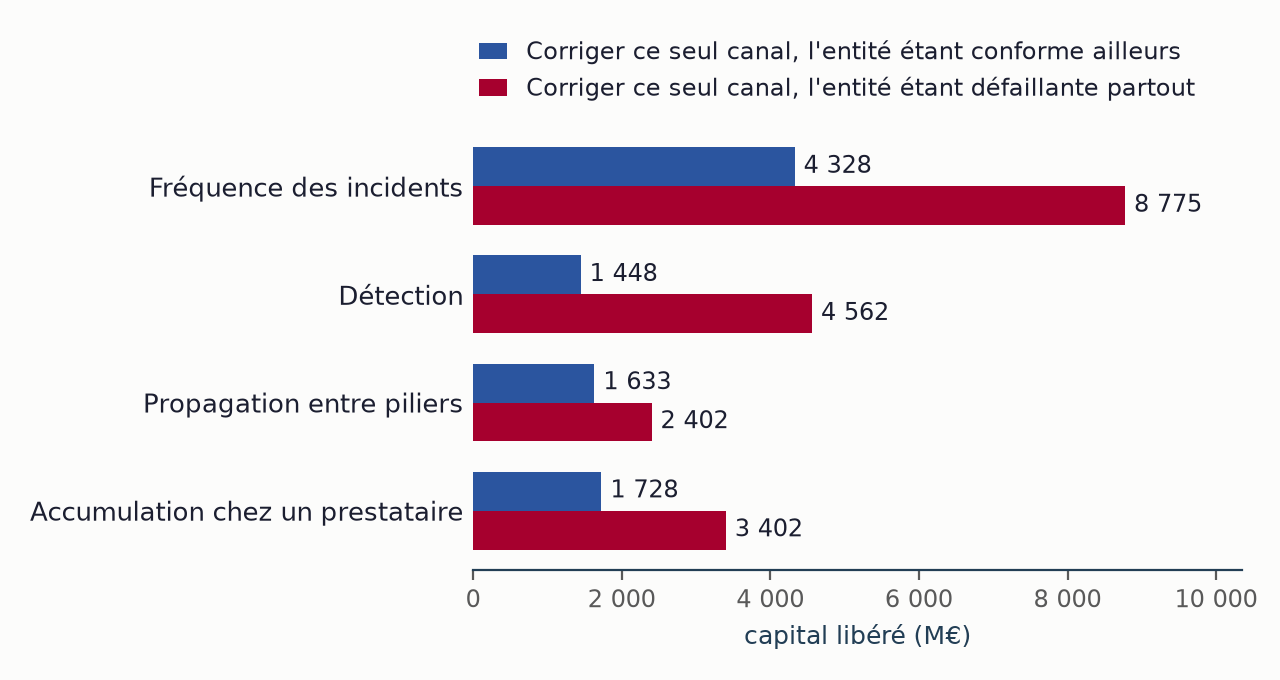
\includegraphics[width=0.72\textwidth]{N1_canaux_note.png}
\caption{Capital libéré par la correction d'un seul canal, selon que l'entité est déjà conforme sur
les trois autres canaux (effet isolé) ou défaillante partout (effet de fermeture), en M\euro{} à
l'échelle du secteur.}
% SOURCES-SCRIPTS: 101 68
\label{fig:canaux-rapport}
\end{figure}

Le facteur se compare d'une lecture à l'autre, non l'écart en euros. Entre les
deux premières lignes, l'écart passe de $8\,860$ à $8\,410$~M\euro{} alors que le facteur monte, la
base conforme passant de $7\,987$ à $6\,664$~M\euro. Les canaux se multiplient presque, le produit
des quatre facteurs isolés étant de $3{,}47$ pour un facteur publié de $3{,}34$
(figure~\ref{fig:treillis-canaux-rapport}). Les quatre effets isolés somment à $9\,138$~M\euro{} et
l'écart de $14\,139$ les dépasse de $5\,001$, l'interaction. Elle correspond à ce que donnerait un
produit des facteurs ($5\,813$~M\euro{} pour un modèle purement multiplicatif) plus qu'à un effet
propre de la cascade (\S\ref{sec:inverse}). Les
trajectoires et la priorisation restent conduites en lecture~B, car elles concernent l'ordre de
remédiation, que le canal ajouté ne déplace pas.

\begin{figure}[H]\centering
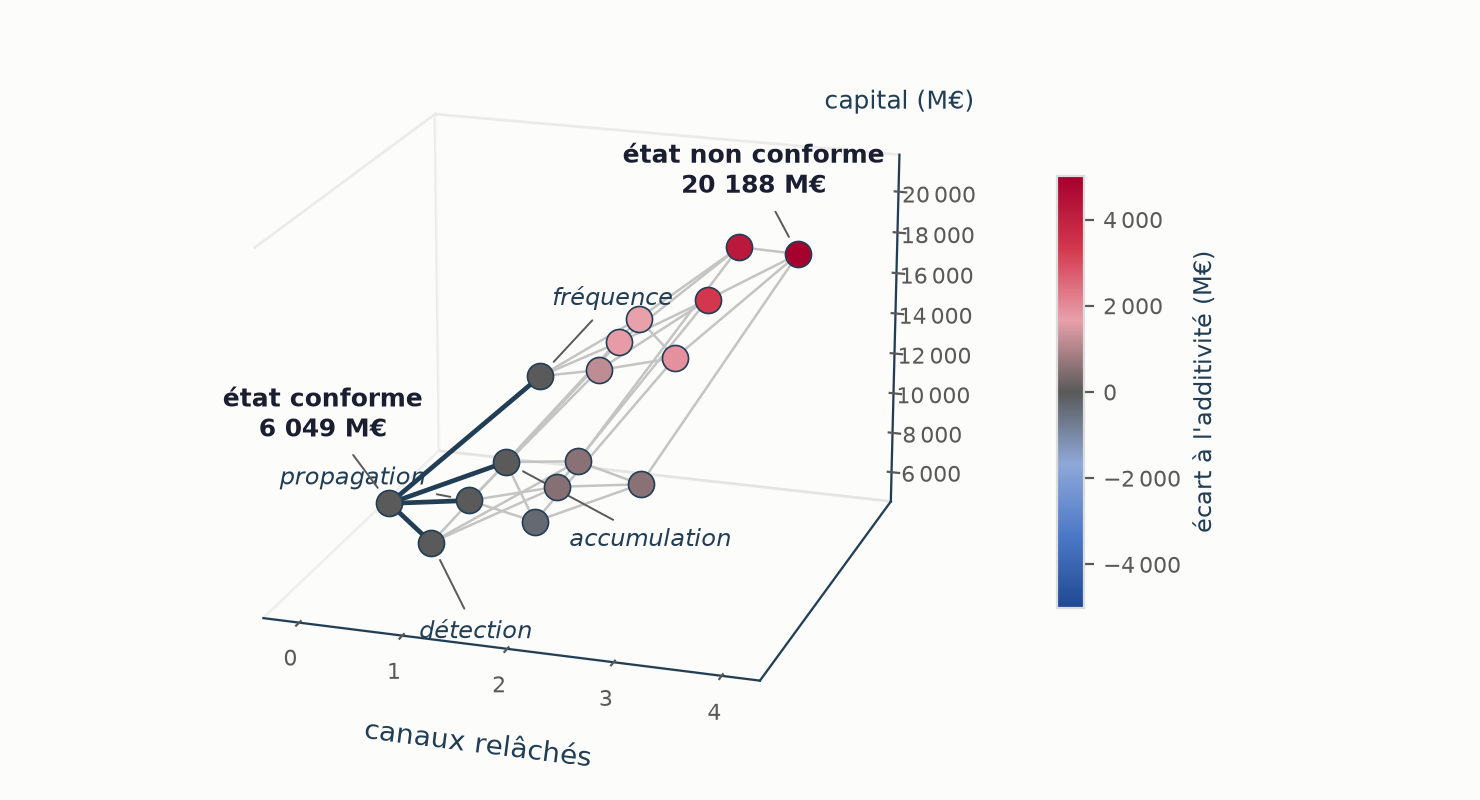
\includegraphics[width=0.95\textwidth]{treillis_canaux.png}
\caption{Les seize configurations des quatre canaux, rangées par nombre de canaux relâchés. La
hauteur est le capital ; les deux extrémités sont les états publiés, $6\,049$ et
$20\,188$~M\euro{}, et tout sommet intermédiaire est une remédiation partielle. Chaque arête monte.
La couleur est l'écart à l'additivité, capital observé moins la somme des quatre effets isolés :
$+5\,001$~M\euro{} au sommet complet, $-330$ sur la seule paire négative, propagation et
accumulation. Le troisième axe sépare les configurations de même rang et ne porte aucune grandeur.}
% SOURCES-SCRIPTS: 68 108
\label{fig:treillis-canaux-rapport}
\end{figure}

Nous obtenons le surcoût $\Delta_{\text{DORA}}=\mathrm{SCR}(\text{NC})-\mathrm{SCR}(\text{C})$, à
graine Monte-Carlo commune, par bootstrap à deux niveaux (multiplicateurs et sévérité), et
$100\,\%$ des tirages sont positifs (tableau~\ref{tab:delta}).

\begin{table}[htbp]\centering\small
\renewcommand{\arraystretch}{1.25}
\begin{tabular}{@{}l cc@{}}
\toprule
& médiane & IC90\,\% \\
\midrule
$\Delta_{\text{DORA}}$ NC vs C (OpRisk) & 7401 & $[2830\,;38793]$ \\
$\Delta_{\text{DORA}}$ PC vs C (OpRisk) & 2556 & $[963\,;12768]$  \\
$\Delta_{\text{DORA}}$ NC vs C (PRC)    & 3668 & $[3201\,;4094]$  \\
$\Delta_{\text{DORA}}$ PC vs C (PRC)    & 1257 & $[1077\,;1466]$  \\
\bottomrule
\end{tabular}
\caption{Surcoût de non-conformité (M\euro), lecture B, bootstrap deux niveaux. Côté OpRisk la
sévérité de queue est ré-échantillonnée sur les $91$ excès réels ; l'intervalle reste large parce
que la queue l'est.}
\label{tab:delta}
\end{table}

La queue d'indice $0{,}60$ explique la largeur de l'intervalle OpRisk ; le surcoût reste positif dans tous les tirages.
Cet intervalle concerne la lecture B. Pour les quatre canaux, seule la dispersion entre graines est donnée (écart-type de $734$~M\euro), sans l'incertitude d'estimation de la queue.
Réinjecter le résidu de conversion de \citet{jacobs2014}, $0{,}523$ en logarithme (facteur $2{,}4$ à $90\,\%$),
laisse l'intervalle PRC étroit et déplace le surcoût de $7\,\%$.

% SOURCES-SCRIPTS: 25 16 43 67 68 100 14 21 74

\section{Décomposition par pilier}

Si l'on bascule un pilier à la fois de conforme à non conforme, le surcoût se décompose selon le
classement $P1>P4>P2>P3>P5$, celui du classement ROOT du modèle qualitatif. Cet accord est attendu et
ne constitue pas une validation indépendante, car les amorces de la cascade sont semées selon ROOT, posé par le même expert que
la matrice dont $W$ est tirée (\S\ref{sec:baremes}).

Les surcoûts isolés ne somment pas au surcoût total, la différence étant une interaction qu'un modèle sans
propagation ne produit pas. Sur la VaR à $99{,}5\,\%$ OpRisk, son signe n'est pas résolu, de $-137$ à
$+1\,395$~M\euro{} sur six graines de $60\,000$ années, positive quatre fois sur six. Elle est
positive sur les six graines en perte moyenne, de $+532$ à $+659$~M\euro{} côté OpRisk et $+827$
côté PRC, et dans la VaR du périmètre PRC, dont le plafond tronque la queue ($+905$~M\euro).

L'attribution par pilier exige donc une règle additive, la valeur de Shapley. Cette
interaction entre piliers ne s'additionne pas à l'interaction de $+5\,001$~M\euro{} entre les quatre
canaux, de signe résolu (\S\ref{sec:kpi}) : elles décomposent l'écart selon deux axes, les piliers et
les canaux, et l'attribution par pilier se lit sur le protocole du tableau~\ref{tab:shapley}.
% SOURCES-SCRIPTS: 16b 20b 68

\section{Allocation du capital par Shapley et Euler}
\label{sec:allocation}

La valeur de Shapley attribue le surcoût aux piliers sources de la non-conformité, interaction
comprise, et indique ainsi qui le supporte. La règle d'Euler, appliquée à la moyenne de queue
de $L$, indique sur quels piliers touchés se loge la perte au-delà du quantile.
% SOURCES-SCRIPTS: 20

\subsection{Attribution par Shapley}

On munit les piliers d'une fonction caractéristique
\[
v(S) \;=\; \mathrm{SCR}\bigl(S \text{ en NC},\ \text{reste C}\bigr)-\mathrm{SCR}(\text{tous C}),
\qquad S \subseteq \{P1,\dots,P5\},
\]
calculée par la cascade sur les $2^5$ configurations à graine Monte-Carlo commune. La valeur de
Shapley
\[
\varphi_j \;=\; \sum_{S \subseteq \{P1,\dots,P5\}\setminus\{j\}}
\frac{|S|!\,\bigl(5-|S|-1\bigr)!}{5!}\,\bigl[v(S\cup\{j\})-v(S)\bigr]
\]
moyenne la contribution de $j$ sur tous les ordres d'arrivée, et
$\sum_j \varphi_j = v(\text{tous}) = \Delta_{\text{DORA}}$ \citep{Shapley1953}. Son
emploi en allocation de capital remonte à \citet{denault2001}, et son usage actuariel sous
Solvabilité~II est documenté \citep{Decupere2011}. Avec cinq piliers, on énumère les $5!$
ordres, sans les algorithmes par échantillonnage \citep{CastroGomezTejada2009, SongNelsonStaum2016}.
Le tableau~\ref{tab:shapley} en donne les valeurs.

\begin{table}[H]\centering\small
\renewcommand{\arraystretch}{1.25}
\begin{tabular}{@{}l rrr c rrr@{}}
\toprule
& \multicolumn{3}{c}{OpRisk} & & \multicolumn{3}{c}{PRC} \\
\cmidrule{2-4}\cmidrule{6-8}
pilier & marginal & $\varphi_j$ & part & & marginal & $\varphi_j$ & part \\
\midrule
P1 gouvernance & 3481 & 3717 & $34{,}0\,\%$ & & 1375 & 1608 & $32{,}4\,\%$ \\
P4 tiers       & 2658 & 2810 & $25{,}7\,\%$ & & 1075 & 1252 & $25{,}3\,\%$ \\
P2 incidents   & 1634 & 1867 & $17{,}1\,\%$ & &  721 &  920 & $18{,}6\,\%$ \\
P3 tests       & 1094 & 1484 & $13{,}6\,\%$ & &  571 &  738 & $14{,}9\,\%$ \\
P5 partage     &  665 & 1048 &  $9{,}6\,\%$ & &  311 &  438 &  $8{,}8\,\%$ \\
\midrule
somme          & 9531 & 10\,927 & $100{,}0\,\%$ & & 4052 & 4957 & $100{,}0\,\%$ \\
\bottomrule
\end{tabular}
\caption{Valeur de Shapley du surcoût $\Delta_{\text{DORA}}$ (M\euro, périmètre financier étudié, trois canaux : fréquence, propagation, détection ; base
conforme $6\,085$ du moteur par pilier, qui s'écarte de quelques pour cent de la lecture~C du tableau~\ref{tab:scretat}).}
% SOURCES-SCRIPTS: 16b
\label{tab:shapley}
\end{table}

Le classement de Shapley reproduit le classement ROOT sur les deux périmètres, en partie
mécaniquement, les amorces étant semées selon ROOT (parts $30/27/18/15/9\,\%$). La part de P1,
$34\,\%$, excède toutefois sa part d'amorce de $30\,\%$, ce qui traduit l'effet propre de la
propagation, P1 étant l'émetteur le plus fort de $W$.
% SOURCES-SCRIPTS: 20

\subsection{Allocation par Euler}

La règle d'Euler \citep{tasche1999} calcule
$C_j = \mathbb{E}\bigl[L_j \mid L \ge \VaR_{99{,}5\,\%}\bigr]$, où $L_j$ est la perte du pilier touché
$j$. Ces contributions somment à $\TVaR_{99{,}5\,\%}(L)$ et non au quantile : c'est une allocation de
la moyenne de queue, lue comme diagnostic de la localisation du capital. Côté PRC, l'allocation est stable et presque plate (P2 $23\,\%$, P4 $23\,\%$, P1 $20\,\%$, P3
$18\,\%$, P5 $17\,\%$), le plafond de sévérité tronquant la queue ($\TVaR = 6\,795 \approx \VaR =
6\,573$~M\euro). Côté OpRisk, les parts moyennes sont stables, mais l'allocation de la queue
extrême ne l'est pas. En effet, avec $\xi \approx 0{,}6 > 0{,}5$, la sévérité est de variance infinie
et le classement conditionnel bascule d'une résolution de simulation à l'autre. Nous retenons donc
l'allocation du périmètre PRC.
% SOURCES-SCRIPTS: 16b

Le besoin de capital publié est partout le quantile $\VaR_{99{,}5\,\%}(L)$ non centré, la perte
attendue d'une non-conformité n'étant pas couverte par une provision. Aucune grandeur de couverture
n'est une TVaR. La mesure de queue ne sert qu'au diagnostic, à deux titres. Elle sert d'abord de
base à l'allocation d'Euler, qui répartit la TVaR et non le quantile. Elle indique aussi la forme de la queue, le rapport
$\TVaR_{99{,}5\,\%}(L)/\VaR_{99{,}5\,\%}(L) \approx 2{,}1$ se comparant à son asymptote
$1/(1-\xi) = 2{,}5$. Ce rapport est de $2{,}10$ à l'état tous non conforme et de $2{,}17$ sur la
calibration de référence. Sous la calibration PRC non plafonnée, $\hat\xi=1{,}033>1$ rend l'espérance infinie, de
sorte que la mesure de queue n'existe pas et ne peut fonder un besoin de capital ; l'allocation du
périmètre PRC porte sur la sévérité plafonnée, dont les moments sont finis.
% SOURCES-SCRIPTS: 20 67 73

\section{Trajectoire du capital}
\label{sec:res-traj}

Le long de la mise en conformité, partant d'une répartition supposée des états (NC~$35\,\%$, PC~$35\,\%$,
C~$30\,\%$), en lecture~B, le capital OpRisk passe de $10\,752$ à $7\,041$~M\euro{} en cinq ans, vers le SCR
conforme. Le surcoût résiduel tend vers zéro, et son intégrale, à un coût de capital près, est le
coût de portage de la non-conformité pendant la remédiation. La bande à $90\,\%$ reste haute en
environnement dégradé, scénario où le capital importe le plus.
% SOURCES-SCRIPTS: 17

\section{Priorisation de la remédiation}
\label{sec:res-prio}

Sous budget contraint, un pilier remédié à la fois, nous énumérons les $120$ ordres, dont
l'optimal, $P1\to P4\to P2\to P3\to P5$, est égal à l'ordre ROOT et distinct de l'ordre glouton par
valeur d'accélération. L'écart de capital intégré entre le pire ordre et l'optimal atteint
$21\,\%$. Remédier au coup par coup le pilier au plus fort gain immédiat coûte plus cher, car les
interactions de cascade imposent de raisonner sur l'horizon entier.
% SOURCES-SCRIPTS: 18

Le test de résistance inverse fixe le capital et cherche les états qui le produisent, la monotonie
du \S\ref{sec:kpi} rendant croissant l'ensemble des configurations atteignant une cible, donc décrit
par ses éléments minimaux. Le canal de fréquence seul atteint $10\,377$~M\euro, soit $1{,}72$ fois
l'état conforme, et les trois autres canaux réunis n'atteignent que $11\,413$ ($1{,}89$ fois).
Toute cible sous le premier seuil se produit par un canal unique, et toute cible au-dessus du second
exige la fréquence. Aucun autre canal seul n'atteint $8\,000$~M\euro{} (\S\ref{sec:inverse}).
% SOURCES-SCRIPTS: 92

\section{Robustesse}
\label{sec:res-robustesse}

Le niveau du capital varie beaucoup avec les leviers testés, l'indice de queue dominant avec
un facteur de l'ordre de $6$. Le signe du surcoût et la priorité de P1 tiennent pourtant sur tous
ces leviers. L'ordre de remédiation optimal ne dépend que des SCR par configuration, et il
est donc invariant aux taux de transition de la chaîne de Markov, qui ne fixent que le calendrier.
% SOURCES-SCRIPTS: 19

Nous menons ces tests à matrice $W$ fixée. Sur l'ensemble admissible (chapitre~\ref{chap:partielle}),
P1 et P4 sont presque à égalité, P1 arrivant premier dans $43{,}6\,\%$ des configurations et P4 dans
$37{,}7\,\%$, avec un écart de regret maximal de $1{,}5\,\%$. P1 et P4 devancent P2, P3 et
P5, et P5 n'arrive jamais en tête. Les rapports post-incident sur-attribuant à la gouvernance, nous
dégradons l'émission de P1 par $W_{1k}\to(1-a)W_{1k}$, et le classement tient jusqu'à $a=0{,}25$
puis bascule vers P4 à $a=0{,}50$. Même à $a=1$, le niveau ne perd que $24{,}8\,\%$, l'équivalent de
$0{,}81$ fois la largeur de la bande d'identification.
% SOURCES-SCRIPTS: 30 64 22 67

\section{Sensibilité aux probabilités de propagation}
\label{sec:sensibilite-propagation}
% SOURCES-SCRIPTS: 15 76 30 66 68

Le niveau de la propagation est un facteur d'échelle posé, qui se stresse, tandis que sa direction
n'est pas identifiable et se borne. Mesurée en élasticités, à perturbation relative de $10\,\%$ d'un paramètre
à la fois, la sensibilité classe les leviers comme suit.

\begin{center}\footnotesize
\renewcommand{\arraystretch}{1.15}
\begin{tabular}{@{}l l r@{}}
\toprule
\textbf{Levier} & \textbf{Statut} & \textbf{Élasticité} \\
\midrule
Indice de queue $\xi$ & estimé & $3{,}79$ \\
Échelle $\sigma$ & estimé & $0{,}97$ \\
Taux de dépassement $p_u$ & estimé & $0{,}82$ \\
Fréquence $\lambda$ & estimé & $0{,}45$ \\
Sur-dispersion $\varphi$ & posé & $-0{,}44$ \\
\textbf{Gain de propagation} $\boldsymbol{g}$ & \textbf{posé} & $\mathbf{0{,}37}$ \\
Seuil $u$ seul & choix de méthode & $0{,}03$ \\
\bottomrule
\end{tabular}
\end{center}

\vspace{4pt}
\noindent La propagation a l'élasticité la plus faible des leviers substantiels, $0{,}37$ contre
$3{,}79$ pour l'indice de queue. Le même classement ressort de l'ablation, qui fait tomber la VaR de
$20\,\%$ en retirant la propagation et de $76\,\%$ en retirant la queue lourde. La thèse ne dépend pas des trois valeurs
posées de $g$, le capital étant croissant en $g$ (\S\ref{sec:invariance-g}). Nous bornons la direction.
À ignorance totale, la largeur de l'ensemble admissible s'élève à $1\,839$~M\euro, soit $34{,}9\,\%$
du socle, et elle croît avec le degré d'ignorance ($336$, $695$, $1\,083$ puis $1\,839$~M\euro{} pour
degrés d'ignorance de $0{,}25$, $0{,}50$, $0{,}75$ et $1$). Le déplacement
conjoint du seuil et des paramètres de queue réajustés ($\xi$, $\sigma$, $p_u$) fait passer le
surcoût de $4\,862$ à $12\,944$~M\euro, sur la base propre du tornado, distincte du chiffre de tête.
Le seuil seul pèse peu ($0{,}03$), et l'incertitude numérique tient d'abord à l'ajustement de la queue.
% SOURCES-SCRIPTS: 81

\section{Comparaison de modèles de dépendance}
\label{sec:benchmark}

Comme la cascade remplace l'agrégation par copule d'un modèle LDA, nous la confrontons à des modèles à copule
de mêmes marges par pilier, à graines communes, sur le périmètre OpRisk. À corrélation
calée, la copule gaussienne retombe sur le SCR de la cascade ($+0{,}1\,\%$ sur une graine,
$+4{,}8\,\%$ en moyenne sur quatre, sous son propre bruit). En queue lourde, le quantile annuel
tient à la perte unique dominante, et le niveau n'identifie pas la dépendance. La Student
($\nu = 4$) le surestime de $17\,\%$ en forçant des co-extrêmes que la cascade ne produit pas
($2{,}28$ piliers extrêmes par année de queue contre $1{,}12$). Le préprint de cascade climatique
\citep{ccrn2026} emploie le même protocole.

Basculer un pilier en non-conformité est cependant une intervention. Le modèle à copule y donne un
surcoût inférieur de $38\,\%$, $6\,760$~M\euro{} contre $10\,927$ pour la cascade, la copule n'ayant
pas de mécanisme de propagation. Son interaction moyenne est nulle par construction, tandis que la
cascade en produit $+560$~M\euro{}. La priorité qu'il implique s'inverse sur P2 et P3. Sa dépendance
ne durcit pas non plus lorsque la conformité se dégrade, alors que c'est le canal de propagation que la non-conformité
déplace ($g$ de $0{,}45$ à $0{,}90$).
% SOURCES-SCRIPTS: 23 80 67

\section{Comparaison avec les cadres réglementaires}
\label{sec:regard-reglementaire}

Sur le même écart de capital entre profil conforme et profil non conforme, trois cadres expriment des
fractions différentes de l'effet de la conformité (tableau~\ref{tab:benchmark-sf}).

\begin{table}[H]\centering\small
\renewcommand{\arraystretch}{1.25}
\begin{tabular}{@{}l r r@{}}
\toprule
\textbf{Cadre} & \textbf{$\Delta$ capital C$\to$NC} & \textbf{part de l'effet cascade} \\
\midrule
Formule Standard (Solvabilité~II) & $0$~M\euro{} & $0\,\%$ \\
LDA-copule (dépendance symétrique) & $6\,760$~M\euro{} & $62\,\%$ \\
Cascade dirigée & $10\,927$~M\euro{} & $100\,\%$ (référence) \\
\bottomrule
\end{tabular}
\caption{Fraction de l'effet DORA que chaque cadre sait exprimer (périmètre financier étudié, trois
canaux, accumulation exclue, protocole du tableau~\ref{tab:shapley}).}
\label{tab:benchmark-sf}
\end{table}

La charge de risque opérationnel de l'équation~\eqref{reg:eq:scrop} ne dépend que du volume. Elle
est identique pour une entité exemplaire et pour une entité défaillante sur DORA. La copule capte
$62\,\%$ de l'effet, par les canaux fréquence et détection, mais manque la propagation.
% SOURCES-SCRIPTS: 27 67

\section{Descente à l'échelle d'une entité}
\label{sec:ancrage}

Pour l'entité notionnelle, le repère forfaitaire de la Formule Standard est d'environ
$450$~M\euro. Le socle sans contagion du périmètre financier étudié vaut $5\,275$~M\euro{} ;
les deux ne se comparent pas. Au niveau du
sinistre unique, le quantile de sévérité ($663$~M\euro) et sa moyenne de queue ($1\,752$~M\euro)
sont en revanche du même ordre que les grandes pertes cyber observées ($1\,288$ à $2\,208$~M\euro). À matrice $W$ et moteur inchangés, une entité d'actifs $A$ reçoit une fréquence et une
sévérité lues à sa taille :
\begin{equation}\label{eq:descente}
\begin{gathered}
\lambda(A)=\lambda_c\Big(\frac{A}{A_c}\Big)^{b_\lambda},\qquad
m(A)=\Big(\frac{A}{A_m}\Big)^{b},\\
X=m(A)\sum_{k\in S_a}Y_k,\qquad
\mathcal{B}(A)=\VaR_{99{,}5\,\%}\Big(\sum_{n=1}^{N}X_n\Big),
\end{gathered}
\end{equation}
où $N$ suit la binomiale négative de moyenne $\lambda(A)$ et de surdispersion $\varphi$, $S_a$ est
l'ensemble des piliers touchés depuis l'amorce $a$ et les $Y_k$ les sévérités GPD calibrées. Nous
estimons les élasticités à $b_\lambda = 0{,}074$ et $b = 0{,}087$, d'où $m = 0{,}854$ à la taille
de l'entité notionnelle.

\begin{table}[htbp]\centering
\small
\begin{tabular}{lrrrr}
\toprule
Lecture & $\lambda$ (an$^{-1}$) & sévérité & SCR $99{,}5\,\%$ & Perte moyenne \\
\midrule
Secteur financier mondial & $21{,}56$ & $\times 1$ & $8\,123$~M\euro & $983$~M\euro \\
Seuil \og{}$\geq 10$ événements\fg{} & $0{,}210$ & $\times 1$ & $488$~M\euro & $9{,}7$~M\euro \\
Seuil \og{}toutes firmes\fg{} & $0{,}100$ & $\times 1$ & $229$~M\euro & $4{,}6$~M\euro \\
$\lambda$ lu à la taille de la cible & $0{,}092$ & $\times 1$ & $198$~M\euro & $4{,}3$~M\euro \\
\textbf{Les deux canaux composés} & $\mathbf{0{,}092}$ & $\mathbf{\times 0{,}854}$ &
$\mathbf{169}$~M\euro & $\mathbf{3{,}6}$~M\euro \\
\bottomrule
\end{tabular}
\caption{Le même modèle lu à plusieurs échelles ; seules la fréquence d'amorce et l'échelle de
sévérité changent. La dernière ligne prend fréquence et sévérité à la taille de l'entité notionnelle.}
\label{tab:echelle}
\end{table}

Diviser $\lambda$ par $235$ divise la perte moyenne par $270$ mais le capital par $48$ seulement, car
le quantile extrême dépend du plus grand sinistre. Le chiffre d'entité est une bande,
$[131{,}5\,;183{,}3]$~M\euro{} sur les $1\,024$ sommets admissibles, qui ne traduit que l'ignorance de
la direction, et les $169$~M\euro{} restent une extrapolation d'ordre de grandeur
(\S\ref{sec:entites-reelles}). À cette échelle, la bande
d'identification mesure $51{,}7$~M\euro. L'indice de queue, parcouru sur son intervalle à $90\,\%$
($\xi \in [0{,}304\,;0{,}831]$), fait varier le
besoin de capital de l'entité de $51{,}5$~M\euro, de $140{,}9$ à $191{,}6$~M\euro.

Le gain de propagation pris à ses trois valeurs d'état ($0{,}45$, $0{,}68$, $0{,}90$) fait passer le
besoin de capital de l'entité de $116$ à $143$ puis $169$~M\euro, soit $+45\,\%$ par le seul canal de contagion
(figure~\ref{fig:invariance-g-rapport}). Le repère forfaitaire reste à $450$~M\euro. Ce scénario d'écartement repose sur une correspondance
posée entre état et $g$. Les correspondances testées entre état et $g$ conservent le signe de l'écart (\S\ref{sec:invariance-g}) ; cette vérification sur grille ne démontre pas la monotonie générale du moteur de marche.
% SOURCES-SCRIPTS: 60 49

\begin{figure}[H]\centering
\figover{S23_invariance_conformite.png}
\caption{Capital d'entité et valeurs du gain de propagation $g$. (a)~Le capital croît avec $g$, sur
vingt points de grille à nombres aléatoires communs, quand la charge forfaitaire ne dépend pas de
l'état. (b)~Cinq correspondances entre état et $g$, de très étroite à large : toutes respectent
l'ordre du capital, et le forfait reste plat. (c)~L'amplitude de l'écart ne dépend que de
l'écartement $g_{NC}-g_C$ ; la valeur retenue est marquée, et elle seule relève du scénario.}
% SOURCES-SCRIPTS: 66 67
\label{fig:invariance-g-rapport}
\end{figure}

\section{Application à quatre entités}
\label{sec:entites-reelles}

L'entité notionnelle est posée à $20\,000$~M\$ d'actifs et $15\,000$~M\euro{} de provisions. Nous
appliquons la méthode à quatre assureurs à partir de leurs rapports SFCR de l'exercice 2024, qui
donnent provisions techniques, fonds propres éligibles et SCR. Le besoin de chaque entité est
$\mathcal{B}(A)$ de l'équation~\eqref{eq:descente}, en point au gain de propagation non conforme et
en bande sur les sommets admissibles. Aucun module DORA n'existant en Formule Standard, ce besoin
relève de l'ORSA (section~\ref{chap:reglementaire}), et son rapport au SCR publié est une mise à
l'échelle, pas une part. Nous désignons les entités par leur classe, car le modèle n'utilise que leur
bilan, leur état de conformité étant supposé.

\begin{center}\small
\renewcommand{\arraystretch}{1.25}
\begin{tabular}{@{}l r r r r r@{}}
\toprule
\textbf{Entité} & \textbf{Actifs} & \textbf{SCR publié} & \textbf{Besoin ORSA} &
\textbf{Bande} & \textbf{Rapport} \\
 & M\euro & M\euro & M\euro & M\euro & \\
\midrule
Assureur non-vie A & $2\,319$ & $425$ & $112$ & $[88\,;122]$ & $26{,}4\,\%$ \\
Assureur non-vie B & $5\,305$ & $812$ & $136$ & $[104\,;146]$ & $16{,}7\,\%$ \\
Assureur vie C & $37\,845$ & $1\,587$ & $196$ & $[149\,;213]$ & $12{,}3\,\%$ \\
\textbf{Assureur vie D} & $\mathbf{309\,800}$ & $\mathbf{14\,800}$ & $\mathbf{294}$ &
$\mathbf{[233\,;316]}$ & $\mathbf{2{,}0\,\%}$ \\
\midrule
\emph{Entité notionnelle} & $19\,231$ & -- & $169$ & $[132\,;183]$ & -- \\
\bottomrule
\end{tabular}
\end{center}

\vspace{2pt}
\noindent Les quatre SCR sont publiés, les deux assureurs non-vie les donnant dans leur état
S.25.01, à $425$ et $812{,}5$~M\euro. Seul le total d'actif de trois entités est déduit, par
l'identité comptable, et l'approximation est conservatrice. Les mêmes états publient également le
module de risque opérationnel. Le repère de $3\,\%$ des provisions donne $54{,}1$ contre $59$ publié
sur la première entité non-vie, et $62{,}1$ contre $39{,}7$ sur la seconde, soit $-8\,\%$ et $+56\,\%$. Ce
repère n'est donc qu'un ordre de grandeur, jamais une borne.

Sur la plus grande entité, $310$~Md\euro{} d'actifs, le besoin représente $2{,}0\,\%$ de son SCR
publié, avec $294$~M\euro{} en point et $[233\,;316]$ en bande. L'écart entre états de conformité
subsiste à toutes les tailles, de $+41\,\%$ à $+49\,\%$. La charge décroît toutefois bien moins vite
que la taille, puisqu'un facteur $134$ sur les actifs ne divise la sévérité que par $1{,}53$ et la
fréquence que par $1{,}44$. Le rapport passe ainsi de $2{,}0\,\%$ à $26{,}4\,\%$.

Un critère de $10\,\%$ du SCR total pour un seul risque de non-conformité, posé et non mesuré, place
la bascule entre $37\,845$ et $309\,800$~M\euro{} d'actifs. Le levier propre des entités, de
$4{,}2$ à $18{,}3\,\%$, module aussi cet ordre de grandeur. L'élasticité corrige l'échelle de la
sévérité, mais sa forme reste celle de grandes institutions financières. L'entité notionnelle, à
$19\,231$~M\euro{} d'actifs, se situe sous cette bascule, dans une zone où la mise à l'échelle reste incertaine. Les $169$~M\euro{} sont donc une extrapolation, dont rien ne garantit qu'elle majore le besoin réel ; le critère de poids dans le SCR ne fixe pas de domaine de validité statistique. Au levier médian des quatre entités ($10{,}0\,\%$), qui donne
$1\,932$~M\euro{} de SCR, la charge en représenterait $9\,\%$, sous le critère. L'argument de taille justifie une réserve d'extrapolation, sans prouver que le chiffre surestime le risque réel.

La thèse concerne l'écart entre états, un rapport, qui survit à une erreur de niveau commune aux
trois états. Comme les entités ne publient pas leur état de conformité, nous mesurons une exposition
sous un état supposé, jamais une non-conformité constatée.
% SOURCES-SCRIPTS: 65

\section{Agrégation au capital total}
\label{sec:agregation-scr}

Sous Solvabilité~II, le risque opérationnel n'entre pas dans la matrice de corrélation du BSCR,
selon l'identité $\mathrm{SCR} = \mathrm{BSCR} + \mathrm{Adj} + \mathrm{SCR}_{Op}$ de la
section~\ref{chap:reglementaire}. Nous comparons deux conventions hypothétiques pour agréger un écart $D$ en ORSA : l'ajouter en entier, comme le SCR opérationnel, après en avoir retranché le risque informatique que celui-ci couvre déjà, ou le traiter comme un module corrélé à $\rho$ avec le BSCR :
\begin{equation}\label{eq:agregation}
\Delta\mathrm{SCR}_{\text{additif}} = D,\qquad
\Delta\mathrm{SCR}_{\rho}=\sqrt{\mathrm{BSCR}^2+2\rho\,\mathrm{BSCR}\,D+D^2}-\mathrm{BSCR}
=\tau(\rho,d)\,D,
\end{equation}
\begin{equation}\label{eq:tau}
\tau(\rho,d)=\frac{\sqrt{1+2\rho d+d^2}-1}{d}
=\rho+\frac{d}{2}\bigl(1-\rho^2\bigr)+O(d^2),\qquad d=\frac{D}{\mathrm{BSCR}} .
\end{equation}
Pour $D$ petit devant le BSCR, la convention corrélée en retient environ $\rho D$, la convention additive $D$. Le BSCR n'étant pas publié, nous le minorons par $\mathrm{SCR}-\mathrm{SCR}_{Op}$ si $\mathrm{Adj}\le0$, et par $\mathrm{SCR}/1{,}3$ si les frais des unités de compte sont nuls ($Exp_{ul}=0$) ; pour les assureurs vie, où ce n'est pas vérifié, les valeurs du tableau ne sont pas des majorants garantis.

\begin{center}\small
\renewcommand{\arraystretch}{1.25}
\begin{tabular}{@{}l r r r r@{}}
\toprule
\textbf{Entité} & \textbf{Écart $D$, contagion} & \textbf{$d = D/\mathrm{BSCR}$} &
\textbf{$\tau$ à $\rho = 0{,}25$} & \textbf{additif / corrélé} \\
 & M\euro & & & \\
\midrule
Assureur non-vie A & $34{,}9$ & $0{,}0954$ & $29{,}4\,\%$ & $3{,}41$ \\
Assureur non-vie B & $44{,}4$ & $0{,}0575$ & $27{,}7\,\%$ & $3{,}62$ \\
Assureur vie C & $62{,}7$ & $0{,}0514$ & $27{,}4\,\%$ & $3{,}65$ \\
Assureur vie D & $86{,}0$ & $0{,}0076$ & $25{,}4\,\%$ & $3{,}94$ \\
\bottomrule
\end{tabular}
\end{center}

\vspace{2pt}
\noindent L'écart $D$, limité à la contagion, est un plancher. À $\rho = 0{,}25$, le facteur $1/\tau$
va de $3{,}4$ à $3{,}9$ pour des tailles dans un rapport $134$, et de $2{,}6$ à $3{,}8$ en lecture de niveau.
L'écart représente $0{,}58\,\%$ à $8{,}21\,\%$ du SCR publié et est reconnu intégralement en convention additive.
Pour l'assureur non-vie~A, le besoin atteint $2{,}21$ fois le plafond de $0{,}3\,\mathrm{BSCR}$ du risque opérationnel.
À $\rho=0{,}25$ (posé), un euro d'écart compte trois à quatre fois plus en additif qu'en corrélé, sans économie reconnue par le régulateur.
% SOURCES-SCRIPTS: 95 65

\section{Détention du capital et transfert du risque}
\label{sec:detenir-transferer}
% SOURCES-SCRIPTS: 60

Le portage annuel est fixé à $\mathrm{CoC}\times\mathrm{SCR}$ : $6\,\%$, puis $4{,}75\,\%$ au 30 janvier 2027 (directive (UE)~2025/2).
Le ratio sinistres/primes de $48{,}5\,\%$ donne une prime d'environ $2{,}1$ fois la perte attendue.
Les $169$~M\euro{} de capital pour $3{,}6$~M\euro{} de perte moyenne donnent un multiple de $47$, contre $8{,}3$ sur le périmètre étudié.

Un traité annuel en excès de perte, sans rétention, cède $\min(L,\ell)$ de la charge $L$, pour une portée $\ell$.
Son coût de financement est
\begin{equation}\label{eq:cout-transfert}
C(\ell)=\frac{\E\bigl[\min(L,\ell)\bigr]}{\mathrm{LR}}
+\mathrm{CoC}\cdot\VaR_{99{,}5\,\%}\bigl(L-\min(L,\ell)\bigr),
\end{equation}
où $\mathrm{LR}$ est le ratio de sinistralité et $\mathrm{CoC}$ le taux de coût du capital. Le minimum,
en $\ell^\star=\mathrm{SCR}=169$~M\euro{}, fait passer le coût de $8{,}0$ à $2{,}9$~M\euro{} par
an, soit $-64\,\%$. Pertes conservées comprises, il passe de $11{,}67$ à $5{,}12$~M\euro{} ($-56\,\%$).
Capacité du marché, exclusions et contrepartie réduisent ce gain idéalisé.

Face au meilleur traité, détenir le risque coûte moins cher au-delà de $64\,\%$ de portée sans allègement de capital,
ou $81{,}5\,\%$ pertes conservées comprises.
Si la conformité ramène $\lambda$ de $0{,}092$ à $0{,}046$, le coût optimal baisse de $60\,\%$.

Une simple mise à l'échelle préserve le rapport détention/transfert. La descente d'échelle change aussi la forme des pertes ;
le seul balayage disponible borne cet effet à $+36\,\%$ (de $2{,}78$ à $3{,}78$).
% SOURCES-SCRIPTS: 58 67
                % ex-10
% =====================================================================
% VERSION ENSAE, REDUCTION SFE (phase 3, 1er octobre 2026) : chapitre 10, robustesse, limites et recommandations.
% Copie a texte constant de chapitres/13_inventaire_hypotheses.tex puis chapitres/13b_donnee_manquante_livrable.tex (devenu la derniere section).
% Ne changent que les titres et les renvois repares, listes dans
% reduction/phase3.md.
% Lu par main_ensae.tex seul : ne jamais le faire lire par main_institut.tex,
% qui garde chapitres/.
% =====================================================================

% ---------------------------------------------------------------------
% STATUT : RÉDIGÉ (transplanté de exploratory/cascade_qualitative/
%          chapitre_robustesse.tex, préambule retiré).
% FAIT (août 2026) : la ligne u_ij est au tableau des paramètres, avec sa
%          sensibilité mesurée par l'échelle de repli du ch. 10, ainsi qu'une
%          ligne pour l'élasticité sévérité/taille calibrée au ch. 5.
% ---------------------------------------------------------------------
\chapter{Robustesse, limites et recommandations}
\label{ch:robustesse}
\label{part:limites}

Sur les plages étudiées, le signe du surcoût de non-conformité et la présence de P1 et P4
parmi les piliers prioritaires résistent aux variantes testées. Le niveau du capital et l'amplitude
de l'écart dépendent de la loi de sévérité, de la fréquence et des paramètres posés, et nous les
lisons donc en écarts, en rapports et en classements. Les tests figurent au
chapitre~\ref{chap:resultats}, l'inventaire des paramètres à l'annexe~\ref{sec:ann-parametres}.

\section{Synthèse de robustesse}

Un verdict \rob{} indique que la conclusion tient aux variantes testées, \ass{} un choix déclaré dont l'effet est
mesuré, \feat{} une propriété recherchée par la construction.

% LONGTABLE ET NON tabular DANS UN center, depuis le 1er octobre 2026 au soir (demande de Kelian). Un
% tabular ne se coupe pas : le tableau partait en bloc sur la page suivante, avec le titre de la
% section, et laissait la page d'ouverture du chapitre presque vide. longtable le pose sous
% l'introduction et le coupe entre deux pages, en-tete repete. Lignes et cellules inchangees.
{\footnotesize
\renewcommand{\arraystretch}{1.3}
\begin{longtable}{@{}p{4.5cm} p{4.6cm} p{4.4cm} c@{}}
\toprule
\textbf{Conclusion} & \textbf{Ce qu'on fait varier} & \textbf{Effet mesuré} & \textbf{Verdict} \\
\midrule
\endfirsthead
\toprule
\textbf{Conclusion} & \textbf{Ce qu'on fait varier} & \textbf{Effet mesuré} & \textbf{Verdict} \\
\midrule
\endhead
\bottomrule
\endlastfoot
L'écart $\Delta_{\text{DORA}}$ entre état non conforme et état conforme est positif, de plusieurs milliers de M\euro{} pour le périmètre financier étudié &
source de sévérité (OpRisk / PRC), famille de copule ($\theta\in[1,4]$) &
facteur ${\sim}1{,}9$ entre sources ; $\Delta_{\text{DORA}}$ varie $<1{,}4\,\%$ sur $\theta$ &
\rob \\
Priorité de remédiation P1 puis P4 (les \emph{sources}) &
cadre de dépendance (cascade vs copule), branchement vs marche &
P1 et P4 en tête dans tous les cadres ; SCR $\pm 4\,\%$ (branchement) &
\rob \\
L'\emph{asymétrie} de $W$ décide de l'ordre entre P1 et P4 &
suppression de la partie antisymétrique de $W$ (3\,000 tirages), placebo par permutation (chapitre~\ref{ch:identifiabilite}) &
sans la direction, P1 et P4 ne se distinguent plus ; l'essentiel du surcoût de contagion reste porté par la partie symétrique &
\ass \\
La cascade est retenue sans couche de Hawkes &
noyau exponentiel puis à retard, logique en deux phases &
non distinguable de la cascade à la résolution disponible (\S\ref{sec:trois-etages}) ; excitation intra-journalière (pic $3{,}3$ h) ; endogénéité de $0{,}551$ à ${\sim}0$ si les
co-occurrences du jour passent en exogène &
\ass \\
Les deux lois du socle prédisent une période qu'elles n'ont pas vue &
origine glissante, douze années notées hors échantillon &
fréquence : couverture $91{,}7\,\%$ pour la binomiale négative contre $75{,}0\,\%$ pour le Poisson, log-score en
sa faveur ; forme de queue non rejetée ($p=0{,}4087$) ; douze années offrent trop peu de puissance, et ce résultat va dans le sens du choix sans le démontrer &
\ass \\
Le besoin de capital \emph{réagit} à la conformité et à la contagion &
score de conformité $q\in[0,1]$, gain $g\in[0{,}05\,;0{,}90]$ &
facteur $3{,}34$ de C à NC sur les quatre canaux ($-53\,\%$ sur le seul score) ; $\times 1{,}6$ sur la plage de $g$ &
\feat \\
Le besoin de capital est une distribution large, pas un point &
incertitude de paramètre (bootstrap deux niveaux) &
facteur ${\sim}2{,}5$ sur le quantile d'un sinistre par la seule incertitude de calibration &
\ass \\
Le \emph{niveau} de sévérité ne tient pas hors échantillon &
notation d'une seule année à la fois, seuil ré-estimé sur l'apprentissage &
quantiles dépassés trois fois trop souvent ; l'échelle de queue dérive de $4{,}00\,\%$ par an,
soit au moins $+24{,}7\,\%$ sur le quantile de sévérité &
\ass \\
Le \emph{signe} de $\Delta_{\text{DORA}}$ ne dépend pas de l'additivité des coûts d'un sinistre &
exposant $\theta\in[0{,}70\,;1{,}30]$ sur le nombre de piliers touchés &
écart de $9\,706$ à $20\,487$~M\euro{} : signe et ordre conservés, \emph{amplitude} non
($76\,\%$ de l'écart publié) &
\ass \\
\end{longtable}
}

\vspace{4pt}
\noindent Les deux premières lignes concernent le signe et l'ordre de grandeur de l'effet DORA et la
hiérarchie des piliers, et tiennent sous les variations testées. La troisième, sur le rôle de la
direction, est assumée : P1 et P4 sont presque à égalité sur l'ensemble admissible, et leur ordre
dépend de la direction posée (chapitre~\ref{chap:resultats}). La quatrième et la cinquième, sur
l'auto-excitation et le comportement prédictif des lois du socle, le sont aussi. La sixième décrit un
capital qui bouge avec la conformité, ce que la Formule Standard ne fait pas
(chapitre~\ref{chap:resultats}). Les trois dernières sont des limites. La queue de sévérité domine
l'incertitude sur le niveau. La dérive de l'échelle de sévérité, unique limite relevée hors
échantillon, déplace ce niveau d'au moins $+24{,}7\,\%$ sur le quantile de sévérité
(\S\ref{soc:sec:backtest}), et l'additivité des coûts d'un sinistre multi-piliers pèse sur l'écart
sans en renverser le signe (\S\ref{sec:additivite-couts}).

% SOURCES-SCRIPTS: 25 29 47 63 61 66 67 74 08h 89

\section{Limites du domaine et limites du travail}
\label{sec:deux-natures-limites}

% SOURCES-SCRIPTS: 110

Deux natures de limites se mêlent dans le tableau et dans le registre de la section~\ref{ch:livrable}.
Les unes tiennent à ce qu'aucune source disponible ne permet à quiconque de calibrer, les autres à ce
que nous avons choisi de ne pas faire.

La direction de la contagion entre domaines de contrôle n'est enregistrée par aucune source. Le
schéma VERIS prévoit le champ du domaine de contrôle défaillant, renseigné dans $0{,}12\,\%$ des
$10\,591$ incidents de sa base publique, et une chronologie datée sur au moins deux étapes, dans
$1{,}19\,\%$. Leur intersection
compte un incident, hors du secteur financier (section~\ref{ch:livrable}). Ces constats établissent une limite des sources examinées ; ils ne prouvent pas l'impossibilité d'identifier la propagation dans tout autre dispositif d'observation.

Le coût d'un sinistre touchant plusieurs piliers n'est observé par aucune source. La sévérité cyber
en euros n'existe à cette profondeur que dans des bases de risque opérationnel bancaire, ce qui
fixe le périmètre de calibration du chapitre~\ref{chap:socle} et motive les réserves d'extrapolation du \S\ref{sec:entites-reelles}. Aucun seuil de validité statistique n'est démontré. Devant ces grandeurs, nous montrons la
non-identifiabilité, calculons des extrema numériques aux sommets de l'ensemble admissible et vérifions que la
conclusion tient sur les points intérieurs testés. L'amplitude du surcoût est un scénario, mais son signe et son ordre sont
des résultats.

Les autres limites relèvent de nos choix. L'élicitation structurée, préparée et diffusée, est restée
sans réponse (supplément, \S\ref{ch:elicitation}). La calibration n'est plus modifiée, sauf pour
corriger des erreurs. Nous citons Hackmageddon, source de structure non recalculable, et publions trois écarts
d'estimation involontaires avec leur sens au lieu de les corriger. Les premières limites se
lèveraient avec le registre d'incidents de la section~\ref{ch:livrable}, les secondes en reprenant
ces choix.

\section{Incertitude du besoin de capital en trois étages}
\label{sec:trois-etages}
\label{sec:etage-modele-hors-bande}

L'incertitude sur le besoin de capital se répartit sur trois étages. Au premier, celui du paramètre, l'intervalle
de confiance de $\xi$ dilate le quantile d'un sinistre d'un facteur $2{,}5$. Le deuxième est
l'identification, la direction de $W$ se lisant en bande (chapitre~\ref{chap:partielle}), et le
troisième le modèle, c'est-à-dire le choix de la famille. Lus sur la même grandeur, la charge annuelle
agrégée du périmètre financier étudié, au calage de référence (sévérité OpRisk), les trois étages donnent, en M\euro{} :
% SOURCES-SCRIPTS: 63 46 48 71 60

\begin{center}\footnotesize
\renewcommand{\arraystretch}{1.25}
\begin{tabular}{@{}l l r@{}}
\toprule
\textbf{Étage, lu sur la charge annuelle} & \textbf{Bande} & \textbf{Facteur} \\
\midrule
Paramètre ($\xi$ sur son IC$_{90}$) & $[3\,042\,;\,27\,152]$ & $8{,}93$ \\
Identification (direction de $W$) & $[6\,858\,;\,8\,697]$ & $1{,}27$ \\
Modèle, axe dépendance & $[5\,322\,;\,9\,806]$ & $1{,}84$ \\
Modèle, axe famille de queue & $[4\,330\,;\,39\,901]$ & $9{,}21$ \\
\bottomrule
\end{tabular}
\end{center}

\vspace{4pt}
\noindent Le quantile annuel amplifie l'incertitude de paramètre, si bien que le facteur
$2{,}5$ ne mesure pas l'effet du paramètre sur le capital. L'étage de modèle est du même ordre que
l'étage de paramètre, et les deux dominent l'identification. Sur l'axe de dépendance, la cascade
($8\,318$~M\euro{} dans cette simulation, $8\,123$ au \S\ref{sec:ancrage} : même calage, deux tirages) se place entre une copule gaussienne et une copule de Gumbel. Ces plages font varier $\xi$ seul, $\sigma$ restant fixé : sans leur covariance, elles ne forment ni des majorants ni un intervalle de confiance conjoint, et nous ne les cumulons pas. La plage des familles est un scénario de modèle, qu'on ne pourrait moyenner qu'avec des poids que rien ne justifie ici. L'ordre d'amorce $P1>P4>P2>P3>P5$, posé par ROOT, ne dépend pas de la famille.

Le diagnostic disponible ne permet pas d'attribuer fiablement le regroupement temporel à une auto-excitation : une
cascade sans auto-excitation, ajustée comme une chronologie réelle, donne un ratio de branchement (nombre moyen d'incidents déclenchés par un incident) de
$0{,}480$ au jour contre $0{,}551$ mesuré. Nous retenons la cascade par parcimonie, puisqu'elle
décrit aussi la structure entre piliers.
% SOURCES-SCRIPTS: 85

\section{Contrôle du moteur d'agrégation}
\label{sec:triangulation-agregation}

La charge annuelle du modèle étant une somme composée, on peut aussi calculer son quantile sans
simuler. L'inversion de Fourier de sa fonction génératrice, méthode numérique distincte de la récursion de \citet{panjer1981}, donne $5\,945$ et $19\,890$~M\euro{} contre $6\,049$ et $20\,188$ par Monte-Carlo.
L'écart, de $0{,}75$ et $0{,}59$ erreur type de la référence simulée, n'est donc pas résolu. L'approximation par perte unique \citep{bockerkluppelberg2005} reste à moins de dix pour cent
au second ordre. Ce contrôle, qui ne teste pas la vérité du modèle, vérifie l'agrégation : le quantile publié ne
diffère pas du quantile calculé sans simulation au-delà du bruit de simulation.

% SOURCES-SCRIPTS: 96

\section{Quantile de sévérité prédictif et robuste}
\label{sec:predictive-robuste}
\label{sec:posture-retenue}

Prendre le quantile à $99{,}5\,\%$ d'une loi estimée en un point, le \emph{plug-in}, est fragile,
car le quantile d'un objet incertain, cité seul, ne rend pas compte de son incertitude. Le quantile
de sévérité prédictif intègre
l'incertitude de paramètre avant le quantile, par mélange des lois sur la distribution bootstrap de
$(\xi,\sigma)$, et donne $645$~M\euro{} contre $657$ pour le \emph{plug-in}, avec un bruit de
simulation de $7$~M\euro{}. Le risque d'estimation n'est donc pas un biais de point à ce niveau, mais
il le devient en profondeur ($+4\,\%$ à $99{,}9\,\%$).

Le quantile robuste, qui prend la borne haute du quantile de sévérité sur l'ensemble d'ambiguïté, atteint
$1\,037$~M\euro{} à $95\,\%$ ($1{,}6$ fois le \emph{plug-in}) et $1\,331$~M\euro{} pour le pire cas
de famille lourde. La robuste à $95\,\%$ est aussi la borne haute de l'intervalle publié, les deux
étant le quantile $95\,\%$ de la même loi bootstrap.

Nous publions donc le \emph{plug-in} avec sa bande, la robuste restant un axe prudentiel déclaré,
pour trois raisons. Le capital de solvabilité est défini comme un quantile de la loi de perte, et une
borne haute sur une famille de lois répond à une autre question. La prédictive, préférable en théorie,
se distingue peu du \emph{plug-in}, son écart n'excédant pas deux fois le bruit de simulation, et l'écart de
sa moyenne au point (5~M\euro) étant du même ordre que ce bruit. Enfin, les postures
robustes sont les moins reproductibles, avec des écarts-types de simulation de $13$, $9$ et
$24$~M\euro{}, celui du point étant nul.

La VaR robuste pourrait servir à dimensionner une couverture ; elle n'est pas utilisée au \S\ref{sec:detenir-transferer}.
Un écart durable entre VaR prédictive et \emph{plug-in} conduirait à revoir ce choix.

% SOURCES-SCRIPTS: 46 51 63

\section{Taux de dépassement et sens des écarts connus}
\label{sec:pu-coherence}

Le modèle POT combine le seuil $u$, le taux empirique de dépassement $p_u$ et les paramètres $(\xi,\sigma)$ des excès. À seuil et échantillon fixés, $p_u$ se calcule par comptage ; il ne constitue pas un paramètre libre supplémentaire. La
calibration publie $u=20{,}03$~M\euro{} et $p_u=0{,}1509$, mais ce seuil laisse $91$ excès sur
$582$ pertes ($0{,}1564$). Le $0{,}1509$ correspond à $88/583$, taux d'un filtrage antérieur. Au
taux cohérent, le quantile de sévérité à $99{,}5\,\%$ passerait de $662{,}78$ à $678{,}60$~M\euro{}
($+2{,}4\,\%$, ou $15{,}8$~M\euro).

À autres paramètres fixés, relever $p_u$ augmente stochastiquement la sévérité du moteur et donc son quantile ; une recalibration complète, incluant $(\xi,\sigma)$ et la fréquence, peut modifier cette conclusion. Nous
le déclarons sans le corriger, car une recalibration déplacerait des
centaines de nombres publiés sans qu'aucun déplacement soit attribuable à la correction. Le tableau
donne le sens des écarts connus.

% LONGTABLE ET NON tabular DANS UN center, depuis le 1er octobre 2026 au soir, meme motif que le tableau de
% synthese du \S 10.1 : passe en bloc a la page suivante, il laissait un tiers de page vide. Le
% « \\* » apres chaque intitule de groupe interdit d'en separer la premiere ligne. Lignes et
% cellules inchangees.
{\footnotesize
\renewcommand{\arraystretch}{1.3}
\begin{longtable}{@{}p{5.6cm} p{2.9cm} p{5.6cm}@{}}
\toprule
\textbf{Écart} & \textbf{Sens} & \textbf{Taille} \\
\midrule
\endfirsthead
\toprule
\textbf{Écart} & \textbf{Sens} & \textbf{Taille} \\
\midrule
\endhead
\bottomrule
\endlastfoot
\multicolumn{3}{@{}l}{\emph{Écarts de calibration et d'incertitude}} \\*
Taux de dépassement gelé ($p_u$) & sous-estime & $+2{,}4\,\%$ sur le quantile de sévérité \\
Couverture réelle de l'IC$_{90}$ de $\xi$ & incertitude sous-estimée & $86\,\%$ au lieu de $90\,\%$ ; demi-largeur à élargir d'environ $10\,\%$ \\
Taux $p_u$, calibré par incident, appliqué à chaque pilier touché & majore & $3{,}66$ incidents matériels par an à l'état conforme, $5{,}67$ aux paramètres de base, contre $3{,}37$ dans la donnée \\
Échelle de sévérité non stationnaire & sous-estime & dérive de $4{,}00\,\%$ par an dans la queue ($p=0{,}0386$), dont la moitié d'inflation monétaire ; au moins $+24{,}7\,\%$ sur le quantile, borne basse (\S\ref{soc:sec:backtest}) \\
\midrule
\multicolumn{3}{@{}l}{\emph{Choix posés, tous deux prudents}} \\*
Charge systémique $a$ & majore & $0{,}60$ posé, au-delà de la borne haute empirique $0{,}22$ \\
Sur-dispersion du moteur $\varphi$ & majore & $9{,}20$ posé contre $2{,}24$ mesuré \\
\midrule
\multicolumn{3}{@{}l}{\emph{Limites de périmètre et de transposition, de sens opposés}} \\*
Attritionnel absent de la donnée & sous-estime & non chiffrable : la base est tronquée à son seuil de collecte, les petits sinistres n'y figurent pas \\
Sévérité non plafonnée à l'échelle d'entité & majore & élasticité sévérité/taille $0{,}087$ $[0{,}026\,;0{,}148]$, presque nulle ; affecte le \emph{niveau} d'entité, et peut modifier les écarts entre états \\
\midrule
\multicolumn{3}{@{}l}{\emph{Hypothèse dont le sens n'est pas déterminable}} \\*
Additivité des coûts au sein d'un sinistre multi-piliers & \textbf{indéterminé} & élasticité de l'écart $1{,}20$ ; $[9\,706\,;20\,487]$~M\euro{} pour $\theta\in[0{,}70\,;1{,}30]$, soit $76\,\%$ de l'écart publié (\S\ref{sec:additivite-couts}) \\
\end{longtable}
}

\vspace{4pt}
\noindent À autres paramètres fixés, le taux de dépassement gelé et la dérive d'échelle font sous-estimer le capital ; la sous-couverture de l'intervalle porte sur l'incertitude, non sur le niveau. Les choix posés vont du côté prudent, sans garantir que le capital majore le risque réel. La dérive de l'échelle
pèse un quart, contre quelques pour cent pour les deux premiers écarts. Son effet sur l'écart
entre états est de $-1{,}9\,\%$, non résolu.

% SOURCES-SCRIPTS: 08b 47 57 60 63 65 74 78 89 90 91 118

\section{Défaillances simultanées et additivité des coûts}
\label{sec:additivite-couts}

À l'état non conforme, $62{,}31\,\%$ des sinistres touchent plusieurs piliers
par la cascade seule, hors choc commun P4 ($73{,}25\,\%$ avec lui), contre $31{,}15\,\%$ à l'état conforme.
L'additivité désigne trois objets différents.

L'addition des coûts entre piliers est une hypothèse non testée : chaque pilier tire une perte calibrée sur des incidents complets.
Sans choc commun P4, les moyennes par incident sont $1{,}38$ pilier (état conforme) et $1{,}93$ (non conforme).
À taux de dépassement élémentaire de base fixé, son quantile à $99{,}5\,\%$ représente $1{,}27$ ou $1{,}58$ fois celui d'un incident.
Le choc P4 du moteur à quatre canaux porte ces valeurs à $2{,}44$ piliers et $1{,}85$ dans l'état non conforme.
Ces rapports chiffrent le double comptage, sans le corriger ni mesurer son effet sur le capital annuel.

Selon les piliers non conformes, le capital est presque
additif, comme le mesure un $R^2=0{,}9945$ sur les $32$ configurations. En fonction des quatre canaux,
il est super-additif en euros, $+5\,001$~M\euro{} d'interaction sur $14\,139$ ($+35\,\%$,
chapitre~\ref{chap:resultats}), car les canaux se composent presque multiplicativement
(\S\ref{sec:inverse}).

Nous faisons varier l'additivité des coûts par un exposant. La perte d'un sinistre touchant $k$ piliers
devient $\bigl(\sum_j X_j\bigr)k^{\,\theta-1}$, et $\theta=1$ redonne le modèle publié. Pour $\theta$ dans $[0{,}70\,;1{,}30]$, l'écart entre états parcourt
$[9\,706\,;20\,487]$~M\euro, soit $76\,\%$ de l'écart publié et $15$~fois l'écart-type de $734$~M\euro{}
entre quatre graines. La plage de $\theta$ est posée ; les élasticités la résument, et un autre intervalle demande un nouveau calcul.

Les élasticités sont de $0{,}95$ à l'état non conforme contre $0{,}39$ à l'état
conforme (facteur $2{,}42$). L'exposant agit seulement sur les sinistres multi-piliers,
ce qui explique cette différence et l'interaction avec la propagation.

Sur toute la plage, l'écart garde son signe et son ordre de grandeur, et seule son amplitude dépend
de l'hypothèse. Son sens n'est pas déterminable, car la mutualisation de la remédiation et la
saturation de la capacité de réponse tirent en sens contraire, et aucune source ne les sépare.
Un plafond adossé à l'exposition, appliqué à chaque sévérité élémentaire, atténue l'effet de l'additivité sans l'annuler.
Il réduit l'écart entre états sans le compenser.

% SOURCES-SCRIPTS: 74 68 69 86 109 118

\section{Recommandations sur la donnée manquante}
\label{ch:livrable}

Les trois sources agrégées échouent pour des raisons distinctes. La chronologie américaine manque de
taxonomie et de volume informatif, SAS OpRisk de résolution temporelle, et VERIS possède les bons
champs sans les renseigner. La proposition~\ref{prop:nonid} précise la donnée qui identifierait $W$.

Un registre d'incidents TIC devrait horodater la survenance au mois ou à la semaine et classer par
domaine de contrôle au lieu du vecteur d'attaque. Il devrait de plus consolider une cause commune en
un événement à $N$ victimes, et consigner pour chaque incident les piliers qui ont cédé. Même sans
horodatage, cette loi jointe distingue une matrice de sa transposée. Sur la matrice publiée, la part
des sinistres multi-piliers passe de $62{,}31\,\%$ sous $W$ à $50{,}77\,\%$ sous $W^\top$.

Le registre d'information du règlement d'exécution \citep{eu2024_2956} identifie les prestataires et
leur sous-traitance, ce qui sert la consolidation des causes communes.

Les deux premiers champs existent dans VERIS, mais sont presque toujours vides (\S\ref{sec:deux-natures-limites}).
Nous recommandons de les rendre obligatoires dans la notification des incidents majeurs,
ce que DORA permet d'imposer au-delà d'une collecte volontaire.
% SOURCES-SCRIPTS: 28 52 08b 98 110
% SOURCES-SCRIPTS: 52 08b

On chiffre cette information en restreignant l'ensemble admissible du chapitre~\ref{chap:partielle}
aux configurations compatibles avec elle, puis en mesurant le rétrécissement de la bande de capital.

\begin{definition}[Valeur d'information d'une contrainte]\label{def:voi}
Soit $\mathcal{W}$ l'ensemble admissible et $\mathrm{SCR}:\mathcal{W}\to\R_+$ la fonctionnelle de
capital. La largeur de bande associée à un sous-ensemble $\mathcal{V}\subseteq\mathcal{W}$ est
\begin{equation}
  L(\mathcal{V}) \;=\; \sup_{W\in\mathcal{V}}\mathrm{SCR}(W)\;-\;\inf_{W\in\mathcal{V}}\mathrm{SCR}(W).
  \label{eq:largeur-bande}
\end{equation}
Une information $\mathcal{I}$ qui restreint l'ensemble à $\mathcal{W}_{\mathcal{I}}\subseteq
\mathcal{W}$ a pour valeur le rétrécissement relatif qu'elle produit :
\begin{equation}
  V(\mathcal{I}) \;=\; 1-\frac{L(\mathcal{W}_{\mathcal{I}})}{L(\mathcal{W})} \;\in\;[0,1].
  \label{eq:voi}
\end{equation}
\end{definition}

Six directions sont documentées au chapitre~\ref{ch:identifiabilite}, dont deux concluantes au \S\ref{sec:bayes}.
Chaque coefficient reste libre entre zéro et son maximum. Filtrer une grille commune ($-S$, $0$ ou $S$ par coefficient)
selon ces directions réduit la plage de $32{,}7\,\%$ en moyenne sur quatre graines ($22$ à $44\,\%$).

La largeur initiale varie de $1\,572$ à $1\,894$~M\euro{} selon la graine. La grille ne garantit pas les extrema continus.
Fixer les dix directions réduit la plage de $57{,}9\,\%$, sans identifier l'amplitude.

Fixer une direction à la fois classe les données manquantes (figure~\ref{fig:voi}).
Quatre dépendances réduisent la largeur de $11{,}2$ à $13{,}3\,\%$ en moyenne ; les deux premières sont absentes du corpus.
Leur ordre varie entre graines. Les cinq dernières réduisent la largeur de $0{,}7$ à $2{,}3\,\%$.
% SOURCES-SCRIPTS: 66 55 33 117

\begin{figure}[H]
  \centering
  \figover{valeur_information_grille.png}
  \caption{Valeur de l'information sur quatre graines. (a)~grille commune, chaque coefficient à $-S$, $0$ ou $S$ : six directions connues réduisent la plage de $32{,}7\,\%$ en moyenne ; barres de la graine de référence. (b)~quelle dépendance documenter en
priorité, moyenne et étendue ; en bleu, celles que le corpus couvre déjà.}
  \label{fig:voi}
\end{figure}
% SOURCES-SCRIPTS: 55 116 117
               % ex-11 et 12
% =====================================================================
% VERSION ENSAE, REDUCTION SFE : conclusion.
% Phase 3 : copie de chapitres/14_conclusion.tex. Phase 4 (1er octobre 2026) : reecrite selon la
% regle n°2 de la mission et ramenee a deux pages, en suivant les consignes MS (situer le point
% d'arrivee, ce qui a pu etre realise, ce qui n'a pu l'etre, la suite possible). Rapport :
% reduction/chapitres/conclusion.md, qui liste ce qui est parti et ou.
% Reprise le 1er octobre 2026 tard le soir (« une ecriture plus humaine ») : registre cale sur
% des memoires d'actuariat publies avant 2022 (style/registre_humain.md), longueur inchangee, la
% derniere page etant pleine. Fond inchange.
% Lu par main_ensae.tex seul : ne jamais le faire lire par main_institut.tex.
% =====================================================================

\chapter*{Conclusion}
\phantomsection
\addcontentsline{toc}{chapter}{Conclusion}
\markboth{Conclusion}{}

\section*{Résultats}
Les montants concernent le risque opérationnel d'origine informatique du périmètre financier étudié, et non celui d'un assureur.
Le besoin de capital passe de $6\,049$ à $20\,188$~M\euro{} entre les états conforme et non conforme des quatre canaux (fréquence, détection, propagation, accumulation),
soit un facteur $3{,}34$. L'écart de $14\,139$~M\euro{} compare deux états posés, sans mesurer un effet observé de DORA.
Son écart-type est de $734$~M\euro{} entre quatre graines de simulation.

Les canaux isolés en expliquent
$9\,138$~M\euro{} et leur interaction $5\,001$~M\euro{}, soit $35\,\%$ de l'écart, ce que donnerait à
peu près un produit des facteurs. Un plan de remédiation doit donc citer l'effet d'un canal fermé
depuis l'état non conforme. Relâcher la seule fréquence fait passer le capital de l'état conforme à
$10\,377$~M\euro{}, et toute cible au-delà de $11\,413$~M\euro{} exige ce canal.

La cascade distingue des ordres d'atteinte qu'un score statique des seuls piliers touchés ne représente pas :
$22$ des $26$ ensembles de piliers changent de criticité (note de $1$ à $10$) selon l'ordre d'atteinte.
La normalisation de Leontief garantit la stabilité de la contagion, cycles compris. Un processus de Hawkes
ne se distingue pas de la cascade à la résolution disponible, et nous retenons la cascade par parcimonie.

La queue de sévérité ($\hat\xi = 0{,}5954$ au seuil publié) et la fréquence d'entrée sont calibrées sur
les données ; la propagation et l'accumulation sont posées. Hors échantillon, la binomiale négative
couvre $91{,}7\,\%$ des années contre $75\,\%$ pour le Poisson, et la forme de la queue n'est pas rejetée
($p = 0{,}4087$), mais douze années donnent peu de puissance. Le niveau de la charge annuelle est rejeté
(Kolmogorov-Smirnov, $p = 0{,}0042$), en raison d'une dérive mesurée de l'échelle de sévérité. La
Formule Standard n'exprime pas cet effet.

% SOURCES-SCRIPTS: 28 39 43 68 92 47 89 91 85 100 74 32

\section*{Non-identifiabilité de la direction}
La direction de la contagion n'est pas identifiable sur les données publiques, et les trois sources
étudiées (chronologie américaine, SAS OpRisk, VERIS) échouent pour des raisons distinctes. La meilleure expérience naturelle disponible,
le choc de chaîne d'approvisionnement MOVEit, a un effet net nul une fois un placebo retranché. Le
schéma VERIS, standard de description d'incidents de la profession, prévoit bien les deux champs
manquants, mais leur intersection n'est renseignée que dans \emph{un} incident sur $10\,591$.

Le socle sans
contagion ne dépend pas de la direction, seule grandeur non identifiable ; il garde des paramètres posés
(surdispersion, accumulation), voir le chapitre~\ref{ch:robustesse}. Au-dessus de lui, dans le calage de référence (sévérité OpRisk), le capital du périmètre financier étudié se situe entre
$6\,858$ et $8\,697$~M\euro{} sur les $1\,024$ sommets de l'ensemble admissible. Cette plage, large de $1\,839$~M\euro{}, est calculée aux sommets et n'intègre pas l'incertitude sur la partie symétrique posée par l'expert.

% SOURCES-SCRIPTS: 30 34 28 110

\section*{Conséquences pour le régulateur et pour l'entité}
Ces trois échecs indiquent la donnée qui rendrait la contagion mesurable : un registre d'incidents.
Il horodaterait la survenance à la semaine et classerait chaque incident selon le domaine de
contrôle en cause, plutôt que selon le vecteur d'attaque. Il consoliderait une cause commune en un
événement unique et consignerait l'ensemble des piliers touchés. La loi jointe de ces ensembles
suffit à distinguer une matrice de sa transposée.

Les deux premiers champs existent déjà dans le schéma VERIS, et la notification d'incident majeur
prévue par DORA peut en rendre le remplissage obligatoire, ce qu'une base déclarative volontaire ne
peut pas. Sur une grille commune, fixer le sens des six dépendances documentées par sept rapports post-incident réduit la plage de $32{,}7\,\%$ en moyenne,
de $22$ à $44\,\%$ selon la graine. Ce résultat dépend de la grille et du barème d'expert. Les dépendances les plus utiles à documenter, dont celle entre
gouvernance et gestion des incidents, en lèveraient chacune de $11$ à $13\,\%$ en moyenne, sans que leur ordre soit
résolu.

% SOURCES-SCRIPTS: 66 55 117

Remédier, détenir ou transférer le risque se comparent ensuite en euros par an, avec une prime de réassurance
calculée sur un ratio de sinistralité de $48{,}5\,\%$. Pour l'entité de $15\,000$~M\euro{} de provisions,
dont le besoin de capital ($169$~M\euro{}) est une extrapolation d'ordre de grandeur, le coût annuel
de détention représente plus de deux fois la sinistralité attendue. Avec le traité en excès de perte idéalisé,
le coût de financement baisse d'environ deux tiers, et de plus de moitié pertes conservées comprises.
La capacité du marché, les exclusions et le risque de contrepartie réduisent ce gain.



% SOURCES-SCRIPTS: 58 65 67

\section*{Limites}
L'élicitation structurée a été préparée et diffusée, mais elle est restée sans réponse (supplément,
\S\ref{ch:elicitation}). La lecture centrale de la direction repose donc sur un barème d'expert
qualitatif. Deux hypothèses pèsent le plus sans être testables sur la donnée : les niveaux de
propagation, posés, et l'additivité des coûts entre piliers touchés. L'élasticité de cette dernière atteint $0{,}95$ à
l'état non conforme contre $0{,}39$ à l'état conforme (\S\ref{sec:additivite-couts}).
Dans les deux cas, le signe et l'ordre de l'écart tiennent sur toute la plage étudiée, mais pas
son amplitude.

Sur les sensibilités étudiées, le signe du surcoût et les deux piliers les plus coûteux, la gouvernance et la gestion des
prestataires tiers, sont conservés. L'ordre de remédiation entre ces deux piliers dépend en revanche du
niveau d'émission de la gouvernance : il tient tant que celle-ci n'est dégradée que du
quart, et bascule à la moitié. Le niveau absolu du capital, du secteur comme de l'entité, est illustratif : l'incertitude de queue impose de le présenter en distribution.

% SOURCES-SCRIPTS: 74 64 65

\section*{Ouvertures}
L'élicitation structurée, si un panel y répondait, resserrerait la bande de capital. Une mesure de la maîtrise des risques par pilier permettrait de remplacer le gain de propagation
posé par une grandeur observée.
                  % ex-13
% Enseignements du stage (ex-14), hors du plan cible de la mission mais EXIGES par les consignes
% MS : enseignements de l'ENSAE appliques, part du maitre de stage et des tiers, prise de recul.
% =====================================================================
% VERSION ENSAE, REDUCTION SFE (phase 3, 1er octobre 2026) : enseignements du stage.
% Copie a texte constant de chapitres/19_enseignements_stage.tex.
% Ne changent que les titres et les renvois repares, listes dans
% reduction/phase3.md.
% Lu par main_ensae.tex seul : ne jamais le faire lire par main_institut.tex,
% qui garde chapitres/.
% =====================================================================

% =====================================================================
% ENSEIGNEMENTS DU STAGE
%
% CHAPITRE PROPRE À LA VERSION ENSAE. Seul main_ensae.tex l'appelle : le barème
% de l'école note sur 6 l'analyse et la réflexion sur le contexte et les outils,
% demande de préciser la part d'influence du maître de stage et des tiers, et
% attend un recul sur l'expérience. Un mémoire d'actuariat n'a rien à porter de
% tout cela, et l'Institut ne le demande pas.
%
% RÉÉCRIT EN ENTIER LE 18 SEPTEMBRE 2026, sur consigne de Kélian. Trois règles
% commandent cette version et il ne faut pas les défaire :
%   - registre strictement factuel et concis. Aucune anecdote, aucune mise en
%     scène, aucun récit d'erreur : la version antérieure portait un paragraphe
%     « sept fois j'ai rédigé... et sept fois la sortie l'a démentie » et une
%     série d'anecdotes de vérification de chiffres, tous retirés ;
%   - PAS DE MENTION D'OUTILS D'IA GÉNÉRATIVE DANS CE CHAPITRE. Le paragraphe
%     d'usage qui y existait depuis le 16 septembre en a été retiré le 18, et il
%     n'a pas à y revenir : ce chapitre porte le recul sur la mission, pas la
%     déclaration d'outillage.
%     ATTENTION, CETTE RÈGLE A CHANGÉ DE SENS LE 21 SEPTEMBRE. Elle ne vaut plus
%     que pour CE fichier. Le mémoire, lui, DÉCLARE cet usage, parce que le § 4.5
%     des Recommandations Jury de l'Institut exige une transparence totale et
%     prévoit l'ajournement << sans besoin d'une autre motivation >> en cas de
%     manquement. La déclaration vit donc à deux endroits, et il ne faut les
%     supprimer ni l'un ni l'autre :
%       - le paragraphe d'usage en fin de résumé (chapitres/01_resume.tex),
%         exigé au § 5.1.c ;
%       - l'annexe d'inventaire (chapitres/23_inventaire_ia.tex), exigée au
%         § 5.1.h.
%   - encadrement nommé et traité sobrement : Hugo Rapior en entreprise,
%     Caroline Hillairet à l'ENSAE. Les répondants au formulaire de relecture,
%     eux, ne sont PAS nommés, décision de Kélian du 9 septembre.
%
% La première personne est admise ici, et ici seulement : le barème de l'école
% exige le recul personnel. Le reste du mémoire reste à la voix impersonnelle.
%
% AUCUN RENVOI VERS LES ANNEXES DÉPORTÉES. Les trois \ref vers sec:ann-harnais
% et celui vers sec:ann-intervalle95 ont disparu avec cette réécriture : leurs
% étiquettes n'existent plus depuis le déport des annexes B, D et E.
% =====================================================================

\chapter*{Enseignements du stage}
\phantomsection
\addcontentsline{toc}{chapter}{Enseignements du stage}
\markboth{Enseignements du stage}{}
\label{ens:ch}
\label{part:stage}

% HARNAIS-HORS-SECTION: chapitre de recul sur la mission. Il ne publie aucun
% resultat chiffre : les seules valeurs qu'il evoque sont etablies et sourcees
% dans le corps du memoire, et il n'en reprend aucune en chiffres.


% Reprise le 1er octobre 2026 tard le soir (« une ecriture plus humaine ») : registre cale sur des
% memoires d'actuariat publies avant 2022 (style/registre_humain.md), « je » du recul personnel
% employe plus franchement. Faits inchanges, aucun nombre ajoute.

\section*{Cadre de la mission}
\label{ens:cadre}

J'ai effectué mon stage chez Nexialog Consulting, cabinet de conseil en risques pour le secteur
financier. La mission portait sur la quantification du besoin de capital associé à la
non-conformité au règlement DORA, qui est le sujet de ce mémoire. Quatre contraintes propres à ce
cadre ont orienté le travail.

\subsection*{Livrables}
Outre le mémoire, le stage a donné lieu à un livrable pour le cabinet : l'analyse actuarielle de
l'édition $2026$ d'une étude de marché sur la cyberassurance en France. Je l'ai co-écrite avec mon
maître de stage, et le cabinet l'a publiée \citep{RapiorKaddouri2026}. Cette étude décrit un
marché observé, alors que je construis un modèle sur des états hypothétiques. Elle constate
également, du point de vue de praticiens qui suivent ce marché, que l'exposition cyber ne se traduit
pas en besoin de capital réglementaire, ce qui est la prémisse du mémoire.

\subsection*{Donnée sous licence}
La base de pertes opérationnelles utilisée pour calibrer la sévérité est sous licence et ne peut pas
être redistribuée. Elle n'est donc pas versionnée avec le code, et un lecteur ne peut pas rejouer la
chaîne de calcul depuis la donnée brute. Ce sont les \emph{sorties} des scripts qui sont versionnées,
et le contrôle porte sur la correspondance entre ces sorties et le document. La traçabilité remplace
ainsi la reproductibilité complète, ce que le rapport indique.

\subsection*{Anonymisation des entités}
L'application à quatre assureurs réels est anonymisée. Les sources sont des rapports publics, mais
le modèle n'utilise que le bilan et l'état de conformité y est supposé : nommer une entité
reviendrait à lui attribuer une non-conformité que rien n'observe. La table de correspondance existe
cependant, dans un script, de sorte que le travail reste vérifiable.

\subsection*{Gel de la calibration}
J'ai gelé la calibration à mi-parcours. Il s'agit d'une décision de conduite de projet : un modèle
qui bouge encore, une fois de nombreux résultats écrits, invalide en silence ce qui a déjà été
rédigé. Le gel sépare la correction d'erreur, toujours autorisée, de la recalibration, qui ne l'est
plus. Son prix figure au chapitre~\ref{ch:robustesse}, où des écarts connus sont publiés chiffrés
sans être corrigés.

\section*{Enseignements de l'ENSAE}
\label{ens:ensae}

Le sujet a mobilisé plusieurs enseignements à la fois. La statistique des valeurs extrêmes sert à
modéliser la sévérité, et les modèles à variable latente gaussienne la dépendance entre états de
conformité. Les processus stochastiques décrivent la dynamique de ces états ainsi que le processus
de branchement. La statistique inférentielle fournit les tests d'adéquation et de couverture, les
méthodes de Monte-Carlo les lois de perte simulées, la théorie des jeux coopératifs l'attribution
par canal, et l'assurance non-vie la charge de capital elle-même.

Deux apports ont pesé davantage que les autres. Le premier est l'économétrie de l'identification :
un paramètre mal estimé appelle davantage de données, un paramètre \emph{non identifié} une autre
approche. Reconnaître qu'un paramètre relevait du second cas a changé la méthode
retenue (chapitre~\ref{ch:identifiabilite}). Le second est la lecture de l'indice de queue comme
condition d'existence des moments, qui m'a permis d'écarter deux variantes de modèle au motif qu'un
moment y cesse d'exister. La programmation scientifique a compté autant que ces deux apports,
car maintenir une chaîne de scripts reproductible pendant plusieurs mois relève de l'ingénierie
logicielle.

\section*{Encadrement et tiers}
\label{ens:encadrement}

L'encadrement a été double. En entreprise, Hugo Rapior, mon maître de stage, a tenu avec moi un
point hebdomadaire, préparé sous la forme d'un jeu de diapositives. À l'ENSAE, Caroline Hillairet,
ma tutrice, a suivi le travail lors d'échanges plus espacés.

Leurs demandes n'ont pas porté sur des calculs. Celles de mon maître de stage m'ont conduit à
retirer des lectures que la mesure ne soutenait pas, et à préciser un vocabulaire dont l'imprécision
masquait une borne prise à l'envers. Celles de ma tutrice ont porté sur le traitement de
l'incertitude et ont donné lieu à deux sections du mémoire, le quantile prédictif et la sensibilité
aux probabilités de propagation. J'en retiens qu'une relecture extérieure est surtout utile parce
qu'elle interroge un énoncé hors du contexte qui l'avait justifié.

Le traitement des processus auto-excités appelle une mention particulière, puisque c'est le domaine
de recherche de ma tutrice. L'écartement de cet outil a été testé contre ses propres variantes de
noyau, puis reformulé en cours de travail en équivalence observationnelle suivie d'un choix de
parcimonie (chapitre~\ref{ch:robustesse}).

\subsection*{Sollicitations extérieures}
J'ai lancé deux sollicitations extérieures. J'ai d'abord demandé à un collègue du cabinet un second
codage en aveugle du corpus de rapports post-incident. Ce codage n'était pas reçu à la date de
rédaction, et le dispositif d'accueil, prêt et testé, ne produit aucune donnée en son absence.

J'ai ensuite sollicité trois praticiens du secteur pour une relecture critique des affirmations
qualitatives du modèle, et les trois ont répondu. Le premier n'en a contredit aucune, mais son
exemple admet deux lectures opposées : il illustre la frontière d'identifiabilité sans la lever. Le
deuxième en a contredit deux et a avancé la cause commune comme explication concurrente de la
contagion, tandis que le troisième conteste les deux mêmes affirmations, ce qui répète le désaccord
sans l'élargir. Ces retours sont déclarés sans être intégrés au modèle, ce qui supposerait de
recalibrer, et ils ne déplacent pas les bornes publiées, calculées sans fixer la direction de
propagation. Les répondants ne sont pas nommés, et le détail figure au
\S\ref{sec:relecture-praticien}.

\section*{Bilan personnel}
\label{ens:retiens}

\subsection*{Méthodes quantitatives et objet réglementaire}
La mission a consisté à traduire un texte réglementaire, qui énonce des exigences d'organisation, en
paramètres d'une loi de perte. Cela suppose de décider ce que le texte permet d'affirmer et ce que
la donnée permet d'estimer, puis de maintenir la distinction entre les deux dans chaque énoncé
publié.

\subsection*{Paramètres estimés, posés et non identifiés}
La modélisation de la conformité DORA mêle trois statuts de paramètre. Certains sont estimés sur
données, d'autres sont posés faute de source, et la direction de propagation entre domaines de
contrôle n'est identifiée par aucune des sources disponibles. Afficher chaque paramètre sous son
statut permet à un tiers de discuter le résultat.

\subsection*{Vérifiabilité des résultats}
En conseil, un résultat doit pouvoir être contrôlé par quelqu'un qui n'a pas fait le calcul.
Rattacher chaque nombre publié au calcul qui le produit répond à cette exigence, et ce travail a
occupé une part importante de mon stage. C'est la différence la plus nette que j'aie observée entre
un exercice académique et une mission.

\section*{Recul sur la démarche}
\label{ens:autrement}

Avec le recul, j'aurais mis en place le dispositif de vérification dès le début du stage : construit
à mi-parcours, il m'a obligé à rattacher après coup chaque section du document à ses scripts.
J'aurais aussi gelé la calibration plus tôt, car plusieurs semaines de recalibrations partielles ont
fait bouger des nombres déjà écrits avant que la décision soit prise.


% BIBLIOGRAPHIE AVANT LES ANNEXES : ordre des consignes MS (sommaire, introduction,
% developpements, conclusion, bibliographie, annexes).
\bibliographystyle{plainnat-fr}
% Interligne simple et entrees resserrees dans la bibliographie (1er octobre 2026, demande de
% Kelian : faire la place des figures remontees du supplement). La police reste le Times 12 des
% consignes MS ; l'interligne 1,5 vaut pour le texte courant, comme dans les tableaux.
{\NoAutoSpacing\singlespacing\small\setlength{\bibsep}{0pt plus 0.5pt}\bibliography{references_ensae}}

% =====================================================================
\appendix
% Plus de page de partie : une ligne « Annexes » au sommaire, en tete de la notice.
\clearpage
\phantomsection
\addcontentsline{toc}{part}{Annexes}

% -----------------------------------------------------------------------------
% NOTICE D'ORGANISATION DES ANNEXES. Les annexes B (demonstrations du socle EVT),
% D (pieces justificatives) et E (complements aux chapitres du corps) ont ete
% deportees le 18 septembre 2026 vers materiel_complementaire/ et ne sont plus
% appelees ; les renvois vers elles passent par la macro \matcomp. Depuis la phase 3
% de la reduction, trois autres contenus sont partis dans supplement/ (S1 a S3) ; les
% quatre etiquettes que le corps vise encore y sont relayees ci-dessous.
% -----------------------------------------------------------------------------
\chapter*{Organisation des annexes et matériel complémentaire}
\addcontentsline{toc}{chapter}{Organisation des annexes et matériel complémentaire}
\markboth{Annexes}{}

Ce rapport garde en annexe les démonstrations du modèle de cascade, la table des paramètres et des
notations, et l'inventaire de l'usage de l'intelligence artificielle générative.

Le \emph{matériel complémentaire} de la version complète du mémoire, destinée à l'Institut des
actuaires (démonstrations des théorèmes standards des valeurs extrêmes, pièces justificatives,
compléments de chapitres), est déposé de façon pérenne sur Zenodo, sous l'identifiant
\texttt{10.5281/zenodo.22874524} :
\url{https://doi.org/10.5281/zenodo.22874524}

Le supplément de ce rapport, auquel conduisent les renvois numérotés S1 à S4, réunit les
adaptations par pilier (S1), les pistes pour de futurs mémoires (S2), le questionnaire
d'élicitation (S3), et les compléments retirés du corps du rapport, dont le protocole d'élicitation
et les retours de praticiens (S4). Il est déposé
au même identifiant Zenodo, dans le fichier \texttt{supplement\_rapport\_ENSAE.pdf}.% ETIQUETTES RELAIS : fichier ecrit par reduction/relais_supplement.py, a relancer apres tout
% deplacement vers le supplement.
% =====================================================================
% ETIQUETTES RELAIS VERS LE SUPPLEMENT, ecrites par reduction/relais_supplement.py :
% ne pas editer a la main, relancer le script apres tout deplacement. Chaque ligne
% redefinit une etiquette que le corps vise et que seul le supplement definit ; elle
% imprime sa place dans le supplement et mene a la notice des annexes.
% HARNAIS-HORS-SCRIPT: etiquettes relais ; les nombres sont des numeros de sections du supplement, pas des resultats.
% =====================================================================
\etiquettesupplement{ch:elicitation}{S4.63}%
\etiquettesupplement{don:fig:mep}{S4.6}%
\etiquettesupplement{sec:inverse}{S1.4.1}%
\etiquettesupplement{sec:kpi}{S1.4}%
\etiquettesupplement{sec:p4-accumulation}{S1.2}%
\etiquettesupplement{sec:relecture-praticien}{S4.68}%


% =====================================================================
% Annexe A revenue du supplement le 1er octobre 2026 tard le soir (« enrichissons le memoire ») :
% c'est l'annexe A du plan cible. Le supplement passe a S1-S4.
% =====================================================================
% VERSION ENSAE, REDUCTION SFE (phase 3, 1er octobre 2026) : annexe A, demonstrations.
% Copie a texte constant de chapitres/15b_demonstrations_cascade.tex.
% Ne changent que les titres et les renvois repares, listes dans
% reduction/phase3.md.
% Lu par main_ensae.tex seul : ne jamais le faire lire par main_institut.tex,
% qui garde chapitres/.
%
% PARTI AU SUPPLEMENT (S5) le 1er octobre 2026 au soir, pour tenir sous 100 pages ; REVENU EN
% ANNEXE A le meme soir, demande de Kelian (« enrichissons le memoire et allons chercher les
% 100 pages ») : c'est l'annexe A du plan cible de la mission. Le supplement passe a S1-S4. Les
% demonstrations sont inchangees ; seule la section sur l'efficience de Shapley est reprise dans
% le registre de la mission (sentence et justification retirees, intertitres en gras supprimes, renvoi
% a « l'annexe des adaptations par pilier » corrige en supplement S1).
% =====================================================================

\chapter{Démonstrations du modèle de cascade}
\label{ann:cascade}

% HARNAIS-HORS-SCRIPT: chapitre de demonstrations de la cascade : memes constantes d'enonce ; les valeurs numeriques correspondantes sont verifiees au chapitre cascade, qui cite ses scripts.

Cette annexe démontre les propriétés énoncées à la section~\ref{sec:formalisation}. Les
notations sont celles du chapitre~\ref{chap:cascade} : $P=\{1,\dots,5\}$, $W\in[0,1]^{P\times P}$
avec $W_{jj}=0$, et la cascade indépendante de la définition~\ref{def:cascade}.

\section*{Forme réduite et descendance espérée (proposition~\ref{prop:reduite})}

\begin{proof}
Par définition du produit matriciel, la somme sur les marches dirigées
$a=v_0\to v_1\to\cdots\to v_n=k$ de $\prod_t W_{v_{t-1}v_t}$ vaut $(W^n)_{ak}$. La série
$\sum_{n\ge0}W^n$ est la série de Neumann de $W$ ; elle converge vers $(I-W)^{-1}$ si et seulement si
$\rho(W)<1$.

Soit $\mathcal C_n(a,k)$ le nombre de chemins vivants de longueur $n$ de $a$ vers $k$, un chemin
étant une marche sans pilier répété. Les arêtes d'un chemin sont distinctes, donc indépendantes, et
un chemin est vivant avec probabilité $\prod_t W_{v_{t-1}v_t}$. Ce n'est pas le cas d'une marche qui
repasse par une arête, celle-ci n'étant tirée qu'une fois. Les chemins formant une partie des
marches, $\mathbb E\,\mathcal C_n(a,k)\le (W^n)_{ak}$. L'indicatrice $\mathbf 1\{k\in S_a\}$ vaut $1$
dès qu'\emph{au moins un} chemin vivant relie $a$ à $k$, donc
$\mathbf 1\{k\in S_a\}\le \sum_{n\ge0}\mathcal C_n(a,k)$ presque sûrement. En prenant l'espérance
puis en sommant sur $k$,
\[
  \mathbb E\,|S_a|=\sum_k \mathbb P(k\in S_a)\le \sum_k\bigl((I-W)^{-1}\bigr)_{ak}
  =\bigl[(I-W)^{-1}\mathbf 1\bigr]_a .
\]
L'inégalité est stricte dès que la série compte des marches qui répètent un pilier, ou deux
chemins distincts vers un même pilier : l'écart mesure ces deux contributions.
\end{proof}

\section*{Sous-criticité par normalisation (proposition~\ref{prop:leontief})}

\begin{proof}
Par construction~\eqref{eq:norm}, $W=(g/s_{\max})\,\mathrm{TRANS}\ge 0$ et, pour toute ligne
$j$, $\sum_k W_{jk}=(g/s_{\max})\sum_k \mathrm{TRANS}_{jk}\le (g/s_{\max})\,s_{\max}=g$, puisque
$s_{\max}$ est la plus grande somme de ligne de $\mathrm{TRANS}$. Pour une matrice à
coefficients positifs, le rayon spectral est majoré par toute norme d'opérateur subordonnée,
en particulier la norme infinie, qui est le maximum des sommes de lignes :
$\rho(W)\le\lVert W\rVert_\infty=\max_j\sum_k W_{jk}\le g\le 1$. Pour $g<1$, on a $\rho(W)<1$ et la
série de Neumann converge donc
et $(I-W)^{-1}=\sum_{n\ge0}W^n$ existe, à coefficients positifs. À la borne $g=1$ du domaine, cette
majoration ne donne que $\rho(W)\le 1$ : la convergence tient alors par la valeur calculée de
$\rho(W)$, strictement inférieure à $1$ (chapitre~\ref{chap:cascade}).
\end{proof}

\section*{Loi exacte de l'ensemble atteint (proposition~\ref{prop:loi})}

\begin{proof}
Fixons $A\ni a$. L'événement $\{S_a=A\}$ est l'intersection de deux événements portant sur des
arêtes disjointes, donc indépendants : (i) aucune arête ne relie $A$ à son complémentaire (sans
quoi $S_a$ dépasserait $A$), et (ii) $a$ atteint tout $A$ par les seules arêtes internes à $A$.
L'événement (i) ne concerne que les arêtes $j\to k$ avec $j\in A$, $k\notin A$, chacune absente
avec probabilité $1-W_{jk}$ indépendamment ; sa probabilité est $B(A)=\prod_{j\in A,k\notin A}(1-W_{jk})$.
L'événement (ii) ne concerne que les arêtes internes à $A$ ; notons $R(A)$ sa probabilité.
Par indépendance, $\mathbb P(S_a=A)=R(A)\,B(A)$.

Pour $R(A)$, on partitionne selon le sous-ensemble $A'$ atteint par les arêtes internes. $A'$
contient $a$, et il est \emph{propre} ($A'\subsetneq A$) si et seulement si $A$ n'est pas atteint
tout entier. Sachant que les arêtes internes atteignent exactement $A'$, aucune arête ne va de $A'$
vers $A\setminus A'$ : cet événement a pour probabilité
$\prod_{j\in A',k\in A\setminus A'}(1-W_{jk})$ et il est indépendant de la réalisation interne à
$A'$. On somme les probabilités de ces sous-ensembles propres, puis on passe au complémentaire :
\[
  R(A)=1-\sum_{\substack{A'\subsetneq A\\ a\in A'}} R(A')\!\!\prod_{j\in A',k\in A\setminus A'}\!\!(1-W_{jk}),
\]
avec $R(\{a\})=1$. La récursion sur les sous-ensembles emboîtés est finie et détermine $R$ de
proche en proche.
\end{proof}

\section*{Monotonie stochastique (proposition~\ref{prop:mono})}

\begin{proof}
On construit un \emph{couplage}. Soit $(U_{jk})$ une famille de variables uniformes sur $[0,1]$
indépendantes, commune aux deux matrices. Pour une matrice $M$, déclarons l'arête $j\to k$
vivante si $U_{jk}<M_{jk}$ ; le graphe obtenu a la bonne loi (arête vivante avec probabilité
$M_{jk}$). Si $W\le W'$ terme à terme, alors $U_{jk}<W_{jk}\Rightarrow U_{jk}<W'_{jk}$ : toute
arête vivante sous $W$ l'est sous $W'$. Le graphe sous $W$ est donc un sous-graphe de celui sous
$W'$, et l'accessibilité étant croissante par ajout d'arêtes, $S_a(W)\subseteq S_a(W')$ presque
sûrement. Pour toute fonctionnelle $\varphi$ croissante pour l'inclusion,
$\varphi(S_a(W))\le\varphi(S_a(W'))$ p.s., d'où la domination stochastique et la monotonie de
l'espérance et des quantiles. Enfin, pour une perturbation antisymétrique $A$, l'entrée $W_{jk}$
croît quand $W_{kj}$ décroît : les deux effets jouent en sens contraire sur $S_a$, la monotonie
en $A_{jk}$ n'a plus lieu, et aucune monotonie coordonnée ne garantit l'optimum aux sommets du pavé $\{|A_{jk}|\le t\,S_{jk}\}$. Leur exploration exhaustive reste un contrôle numérique limité.
\end{proof}

\section*{Dépendance à l'ordre et co-occurrence (propositions~\ref{prop:ordre} et~\ref{prop:nonid})}

\begin{proof}
\emph{Ordre.} Pour une chaîne de deux piliers, $\ell(i,j)=\mathrm{ROOT}_i\,\mathrm{TRANS}_{ij}$ et
$\ell(j,i)=\mathrm{ROOT}_j\,\mathrm{TRANS}_{ji}$ : l'invariance par permutation équivaut à
$\mathrm{ROOT}_i\,\mathrm{TRANS}_{ij}=\mathrm{ROOT}_j\,\mathrm{TRANS}_{ji}$. Une invariance valable
pour toute longueur l'impose en particulier aux chaînes de deux piliers, d'où la nécessité. Au-delà
de deux piliers, la condition ne suffit pas : même avec $\mathrm{TRANS}$ symétrique et des poids
d'amorce égaux, $\ell(1,2,3)$ et $\ell(1,3,2)$ diffèrent dès que
$\mathrm{TRANS}_{12}\mathrm{TRANS}_{23}\neq\mathrm{TRANS}_{13}\mathrm{TRANS}_{32}$. Le barème donne
$\mathrm{ROOT}_1\,\mathrm{TRANS}_{12}\neq\mathrm{ROOT}_2\,\mathrm{TRANS}_{21}$, donc l'ordre de la paire (P1, P2) change la vraisemblance. La différence des criticités arrondies se vérifie séparément dans l'exemple numérique ; elle ne découle pas en général d'une différence de vraisemblance. Un
score additif est une fonction de l'ensemble. Une copule, échangeable ou non, décrit la loi jointe
des indicatrices de défaillance, donc elle aussi une fonction de l'ensemble atteint et non de
l'ordre d'atteinte. Aucun des deux ne reproduit cette dépendance.

\emph{Co-occurrence.} La décomposition $W=\tfrac12(W+W^\top)+\tfrac12(W-W^\top)=S+A$ est
unique car $S$ est symétrique, $A$ antisymétrique, et cette somme directe est celle des
matrices en parties symétrique et antisymétrique.

(i) Pour que $j$ et $k$ soient tous deux atteints depuis une amorce $a\notin\{j,k\}$, il faut au
moins deux arêtes vivantes, événement de probabilité $O(\lVert W\rVert^2)$. Depuis l'amorce $j$,
le pilier $k$ est atteint par l'arête directe avec la probabilité $W_{jk}$, et par tout autre
chemin, de longueur au moins deux, avec une probabilité $O(\lVert W\rVert^2)$ ; symétriquement
depuis l'amorce $k$. En sommant sous l'amorce uniforme, la probabilité de co-occurrence vaut
$r\,(W_{jk}+W_{kj})+O(\lVert W\rVert^2)$, et le terme d'ordre un, $2r\,S_{jk}$, est le même pour
$W$ et pour $W^\top$.

(ii) Deux contre-exemples suffisent. Sous une amorce non uniforme de poids $r_a$, le terme
d'ordre un devient $r_j W_{jk}+r_k W_{kj}$, qui change par transposition dès que $r_j\neq r_k$ et
$W_{jk}\neq W_{kj}$. Sous l'amorce uniforme, prenons trois piliers avec $W_{12}=W_{13}=w>0$ et
toutes les autres entrées nulles. Sous $W$, une amorce en $1$ touche $2$ et $3$ ensemble avec la
probabilité $w^2$, si bien que la paire $\{2,3\}$ co-occurre avec la probabilité $r\,w^2>0$. Sous
$W^\top$, les seules arêtes vont de $2$ et de $3$ vers $1$, et aucun sinistre ne touche $2$ et $3$
ensemble. Les deux matrices ont la même partie symétrique : la co-occurrence d'ordre deux
distingue la fourche du collisionneur, ce qui est la structure en V de l'identification des
graphes causaux \citep{verma1990equivalence}.

(iii) Un changement de signe de $A$ modifie la loi de l'ensemble atteint, donc la loi de la perte
et le SCR en général ; la section~\ref{sec:verif-proprietes} en donne la mesure sur la matrice
publiée.
\end{proof}

\section*{Efficience de la valeur de Shapley}
\label{sec:ann-efficience-shapley}

Le chapitre~\ref{chap:resultats} attribue le surcoût de capital aux piliers par la valeur de
Shapley, dont les parts somment à cent. Cette somme est la propriété d'efficience
\citep{Shapley1953}. Elle permet de présenter l'attribution comme une \emph{partition} du surcoût,
et non comme une pondération arbitraire.

\begin{proposition}[Efficience]
\label{prop:efficience}
Soit $v$ une fonction caractéristique sur $\{1,\dots,n\}$ avec $v(\emptyset)=0$, et
\[
  \varphi_i \;=\; \frac1n \sum_{u \subseteq \{1,\dots,n\}\setminus\{i\}} \binom{n-1}{|u|}^{-1}
                  \bigl[v(u \cup \{i\}) - v(u)\bigr].
\]
Alors $\sum_{i=1}^{n} \varphi_i = v(\{1,\dots,n\})$.
\end{proposition}

\begin{proof}
La démonstration repose entièrement sur la réécriture du poids. Pour $|u|=s$,
\begin{equation}
  \frac1n \binom{n-1}{s}^{-1} \;=\; \frac1n \cdot \frac{s!\,(n-1-s)!}{(n-1)!}
  \;=\; \frac{s!\,(n-s-1)!}{n!},
  \label{eq:poids-shapley}
\end{equation}
de sorte que $\varphi_i$ est exactement la moyenne, sur les $n!$ permutations de
$\{1,\dots,n\}$, de la contribution marginale de $i$ à l'ensemble de ses prédécesseurs. En effet,
un sous-ensemble $u$ de cardinal $s$ ne contenant pas $i$ est l'ensemble des prédécesseurs de $i$
dans exactement $s!\,(n-s-1)!$ permutations : $s!$ ordres pour les éléments de $u$, puis
$(n-s-1)!$ pour ceux qui suivent $i$. En notant $\Pi$ l'ensemble des permutations et $P_i(\pi)$
les prédécesseurs de $i$ dans $\pi$,
\[
  \varphi_i \;=\; \frac{1}{n!} \sum_{\pi \in \Pi}
              \bigl[v\bigl(P_i(\pi) \cup \{i\}\bigr) - v\bigl(P_i(\pi)\bigr)\bigr].
\]
Sommons alors sur $i$ \emph{à permutation fixée}. Si $\pi = (\pi(1),\dots,\pi(n))$, posons $S_0=\emptyset$ et $S_j=\{\pi(1),\dots,\pi(j)\}$ pour $1\le j\le n$. Ainsi $P_{\pi(j)}(\pi)=S_{j-1}$, et la somme des contributions marginales est télescopique :
\[
  \sum_{i=1}^{n} \bigl[v\bigl(P_i(\pi)\cup\{i\}\bigr)-v\bigl(P_i(\pi)\bigr)\bigr]
  \;=\; \sum_{j=1}^{n} \bigl[v(S_j)-v(S_{j-1})\bigr]
  \;=\; v(\{1,\dots,n\}) - v(\emptyset),
\]
et cette valeur ne dépend pas de $\pi$. En moyennant sur les $n!$ permutations,
$\sum_i \varphi_i = v(\{1,\dots,n\})$, puisque $v(\emptyset)=0$.
\end{proof}

L'efficience fait de l'attribution une partition du surcoût, quels que soient l'interaction et son
signe : rien n'est perdu ni compté deux fois. Elle ne fait pas de la part d'un joueur une
prédiction de ce qu'on obtiendrait en l'écartant seul ; cette prédiction est la contribution
marginale, qui ne somme pas au total. Le chapitre~\ref{chap:resultats} tient cette distinction
entre les lectures d'un même canal, et le supplément S1 donne l'identité correspondante pour
chaque colonne. Une part de Shapley est donc une convention d'attribution, pas un budget de
remédiation : deux des quatre canaux du modèle sont bornés et non calibrés.

La réécriture~\eqref{eq:poids-shapley} rend aussi le calcul praticable : elle ramène l'évaluation à
une moyenne sur les permutations, forme sur laquelle reposent les algorithmes d'approximation en
temps polynomial \citep{CastroGomezTejada2009, SongNelsonStaum2016}, nécessaires quand la dimension
croît. Avec cinq piliers, les $5!$ permutations et les $2^5$ valeurs de $v$ sont énumérées en
entier : les valeurs publiées sont exactes au bruit de simulation de $v$ près, sans erreur
d'approximation combinatoire.
        % A, ex-A (le supplement l'appelait S5)
% =====================================================================
% VERSION ENSAE, REDUCTION SFE (phase 3, 1er octobre 2026) : annexe B, parametres et notations.
% Copie a texte constant de chapitres/17b_table_parametres.tex puis chapitres/16_notations.tex, les deux anciennes annexes devenant les sections B.1 et B.2.
% Ne changent que les titres et les renvois repares, listes dans
% reduction/phase3.md.
% Lu par main_ensae.tex seul : ne jamais le faire lire par main_institut.tex,
% qui garde chapitres/.
% =====================================================================

% =====================================================================
% TABLE DES PARAMÈTRES  --  annexe.
%
% REMISE DANS LE MÉMOIRE LE 18 SEPTEMBRE 2026, quelques heures après le déport
% des annexes B, D et E. Elle vivait au \S sec:ann-parametres de l'annexe D
% (17_pieces_justificatives.tex) et elle est partie avec elle ; Kélian a demandé
% de la remettre le jour même. Elle a été RETIRÉE du fichier déporté, pas
% recopiée : le même tableau à deux endroits divergerait.
%
% POURQUOI ELLE SEULE REVIENT, quand les vingt et une autres sections de
% l'annexe D restent dehors. C'est la table qu'un jury lit en premier pour
% savoir ce qui est calibré, ce qui est posé et ce qui n'est pas identifié, et
% le chapitre 11 annonce qu'elle existe « pour qu'aucun chiffre du mémoire ne
% soit sans origine déclarée » : la laisser dehors rendait cette phrase fausse.
%
% ELLE EST EN longtable ET NON EN tabular, depuis le 17 août 2026. Un tabular ne
% peut pas se couper entre deux pages : il débordait de 102 pt et hyperref
% émettait l'annotation hors page qui accompagne toujours ce débordement.
%
% SES NEUF SCRIPTS SOURCES SONT NÉCESSAIRES. La ligne
% « % SOURCES-SCRIPTS: 08b 22 25 34 47 60 67 99 43 » couvre les soixante et
% quelques nombres de la table ; en retirer un sort des valeurs du contrôle.
% =====================================================================

\chapter{Paramètres et notations}
\label{sec:ann-parametres}

\section{Nature et sensibilité des paramètres}

Trois natures sont distinguées : calibré sur données (avec son incertitude),
\emph{posé} par jugement d'expert ou choix normatif (non identifiable, cf.\
chapitre~\ref{ch:identifiabilite}), et semi-ancré sur un proxy externe non
spécifique au périmètre.

\vspace{0.25cm}
% PASSEE DE tabular A longtable LE 17 AOUT 2026. Cette table tenait sur une page tant que rien
% ne la precedait dans le chapitre ; l'ajout de la section sur le dispositif de verification l'a
% decalee et elle a debordé de 102 pt, avec l'annotation hyperref hors page qui accompagne
% toujours ce debordement. Un tabular NE PEUT PAS se couper entre deux pages : le piege est
% documente et il vient de mordre. longtable le peut, et l'en-tete se repete.
{\footnotesize
\renewcommand{\arraystretch}{1.28}
\begin{longtable}{@{}>{\raggedright\arraybackslash}p{2.7cm}
                    >{\raggedright\arraybackslash}p{2.6cm}
                    >{\raggedright\arraybackslash}p{1.7cm}
                    >{\raggedright\arraybackslash}p{4.0cm}
                    >{\raggedright\arraybackslash}p{3.6cm}@{}}
\toprule
\textbf{Paramètre} & \textbf{Valeur} & \textbf{Nature} & \textbf{Justification} & \textbf{Sensibilité du SCR} \\
\midrule
\endfirsthead
\toprule
\textbf{Paramètre} & \textbf{Valeur} & \textbf{Nature} & \textbf{Justification} & \textbf{Sensibilité du SCR} \\
\midrule
\endhead
\bottomrule
\endlastfoot
Queue de sévérité $\xi$ & $0{,}5954$ (OpRisk, chiffre de tête) ; PRC $1{,}03$ ; $0{,}90$ posé en pire cas de modèle & calibré, incertain & GPD sur pertes réelles ; hétérogène par catégorie ($0{,}87$--$1{,}37$) & \textbf{forte} : de $0{,}60$ à $0{,}38$ quand le seuil monte au-dessus de celui retenu, dans l'IC90 $[0{,}30\,;0{,}83]$ ; pilote la queue \\
Échelle GPD $\sigma$, seuil $u$, $p_u$ & $57{,}97$ M\euro{} ; $20{,}03$ M\euro{} ; $0{,}15$ & calibré & POT au percentile $84{,}4$ ; $p_u$ gelé et en écart de $+3{,}6\,\%$ avec ce seuil, effet chiffré au \S\ref{sec:pu-coherence} & modérée (via la queue) \\
Fréquence $\lambda$ & ${\sim}21{,}6$/an (OpRisk) & convention de calage & événements collectés / 27 ans ; période à réconcilier & sous-linéaire sur le niveau \\
Multiplicateur de fréquence par état & $\times 1{,}525$ partiel ; $\times 2{,}487$ non conforme ($\lambda$ de $21{,}56$ à $53{,}62$) & semi-ancré & parts Hackmageddon et fourchettes posées sur des effets publiés (chapitre~\ref{chap:multietats}) ; aux bornes, $\lambda$ de $41{,}7$ à $65{,}6$ & \textbf{forte} : canal dominant du chiffre de tête \\
Sur-dispersion $\phi$ & $9{,}20$ & \textbf{posé} (prudent) & $2{,}24$ mesuré sur la série annuelle détendancée, maintenu entre scénarios & élasticité $-0{,}44$ sur l'écart entre états \\
Choc commun fréquence $a$ & $0{,}60$ & \textbf{posé} (prudent) & dépasse l'IC empirique haut ($0{,}22$) : conservateur & enveloppe le modèle à paquets ($\times 2{,}5$) \\
Structure $W = g\,\texttt{TRANS}/\max_k s_k$ & classeur qualitatif & \textbf{posé} / normatif & jugement d'expert consigné ; direction non identifiable & l'asymétrie départage les deux piliers de tête ; l'essentiel du surcoût de contagion vient de la partie symétrique \\
Gain de propagation $g$ & $0{,}90$ base ; par état $0{,}45/0{,}68/0{,}90$ & \textbf{posé} & amplitude de $W$, bornée par Leontief $\rho(W)\le g<1$ & \textbf{levier} : $\times 1{,}6$ sur $[0{,}05\,;0{,}90]$ \\
Score de conformité $q$ / états & continu $[0,1]$ (ou NC/PC/C) & \textbf{posé} & décrit le profil, subsume 3 ou 5 niveaux & \textbf{levier} : $-53\,\%$ de NC à C sur le seul score ; facteur $3{,}34$ sur les quatre canaux \\
Multiplicateur de matérialité par état & $0{,}85/1{,}00/1{,}20$ & \textbf{posé} & module $p_u$ selon la conformité & modérée (canal détection) \\
Charge systémique $\gamma$ & $0{,}68$ & semi-ancré & proxy concentration cloud (AWS+Azure+GCP, Synergy 2025) & modérée \\
Seuil de crise $\theta_{\text{crise}}$ & $-2{,}5$ & \textbf{posé} & déclenche le régime de co-mouvement extrême & agit sur la seule queue crise \\
Probabilités d'état $P(\text{NC/PC/C})$ & $0{,}35/0{,}35/0{,}30$ & semi-ancré & enquêtes conformité DORA ${\sim}50\,\%$ non conformes (Deloitte, ESA) & déplace le mélange, pas les états \\
Copule de dépendance $\theta$ & Gumbel $1{,}8$ & \textbf{posé} & queue supérieure entre briques & \textbf{négligeable} : $\Delta_{\text{DORA}}$ $<1{,}4\,\%$ sur $[1,4]$ \\
Excès de source $u_{ij}$ & $\operatorname{logit}p_{ij}=\operatorname{logit}p_j+u_{ij}$ & \textbf{non identifié} & la direction elle-même ; normalisation $\sum_i u_{ij}=0$ (repérage, non information) & mesurée par l'échelle de repli (ch.~\ref{chap:partielle}) : rang~$1$ capte $74\,\%$ et resserre les bornes de $25\,\%$ ; à $u=0$ P1 et P4 deviennent indiscernables \\
Élasticité sévérité/taille $b$ & $0{,}087$ $[0{,}026\,;0{,}148]$ & calibré, tronqué & EMV lognormale tronquée au seuil de collecte (ch.~\ref{chap:donnees}) & faible : $\times 0{,}86$ sur la sévérité transposée \\
Plafond de sévérité & $40$ M\euro{} & \textbf{posé} & capacité de réassurance ($\xi\ge 1$) ; appliqué par pilier touché & borne la queue extrême \\
\end{longtable}
}

\vspace{4pt}
% SOURCES-SCRIPTS: 08b 22 25 34 47 60 67 99 43 76

Les paramètres à forte sensibilité sont soit calibrés sur données (la queue $\xi$, dont
l'incertitude est chiffrée), soit des \emph{leviers voulus} ($g$, $q$, le multiplicateur de
fréquence), qui portent l'effet de la conformité et de la contagion sur le capital. Les paramètres purement posés qui
ne sont pas des leviers ($\theta$ de copule, $\gamma$, $\theta_{\text{crise}}$, probabilités d'état,
matérialité) ont une influence faible à modérée et documentée. Aucune conclusion ne
repose sur un paramètre à la fois non calibré \emph{et} déterminant hors de son rôle attendu.

\section{Table des notations}

% MIGRÉ depuis memoire/main.tex (plages 3230-3259).
% RELECTURE FAITE (août 2026) : la table héritée ne portait AUCUN symbole du
% modèle de cascade (W, S, A, TRANS, ROOT, g, s_j, e_j, R_0, t, kappa), alors
% que c'est le modèle central. Elle est réécrite et organisée en cinq blocs.
\label{not:ann:notations}

\noindent Les symboles sont regroupés par brique du modèle, dans l'ordre où le mémoire les
introduit. La colonne de droite renvoie au chapitre qui les définit.

% LONGTABLE ET NON TABULAR. Un tabular ne peut pas se couper : la table dépassait le
% bas de page, et hyperref plaçait alors les liens \ref des sept dernières lignes à des
% coordonnées NÉGATIVES (sept avertissements « Annotation out of page boundary » à la
% compilation). Les renvois fonctionnaient mais pointaient sur la mauvaise page du PDF.
% longtable répartit la table sur plusieurs pages et rejoue l'en-tête à chaque page.
\renewcommand{\arraystretch}{1.22}
{\small
\begin{longtable}{>{\raggedright}p{3.3cm} >{\raggedright\arraybackslash}p{10.2cm} c}
\toprule
\rowcolor{lightblue}
\textbf{Symbole} & \textbf{Signification} & \textbf{Ch.} \\
\midrule
\endfirsthead
\toprule
\rowcolor{lightblue}
\textbf{Symbole} & \textbf{Signification} & \textbf{Ch.} \\
\midrule
\endhead
\bottomrule
\multicolumn{3}{r@{}}{\footnotesize\itshape suite page suivante} \\
\endfoot
\bottomrule
\endlastfoot
\multicolumn{3}{@{}l}{\emph{\textcolor{navy}{Piliers et cascade dirigée}}} \\
$P_1,\dots,P_5$ & Les cinq piliers DORA : gouvernance, gestion des incidents, tests de résilience, prestataires tiers, partage d'informations & \ref{chap:cascade} \\
$\mathrm{TRANS}$ & Matrice d'influence brute du classeur qualitatif, asymétrique, non normalisée & \ref{chap:cascade} \\
$\mathrm{ROOT}$ & Propension de chaque pilier à \emph{amorcer} une chaîne ; répartit les amorces du moteur & \ref{chap:cascade} \\
$\mathrm{GBASE}$ & Gravité intrinsèque de chaque pilier s'il cède seul, barème ordinal du modèle qualitatif, absent du moteur de capital & \ref{chap:cascade} \\
$s_j$ & Somme de la ligne $j$ de $\mathrm{TRANS}$ ; $s_{\max}=\max_j s_j$ & \ref{chap:cascade} \\
$g$ & Gain de propagation, part de contagion du pilier le plus exposé. \textbf{Mesure une criticité, jamais un montant} : à ne pas confondre avec l'échelon de sévérité par pilier & \ref{chap:cascade} \\
$W$ & Matrice de contagion normalisée à la Leontief, $W=g\,\mathrm{TRANS}/s_{\max}$. \textbf{Convention : $W_{jk}$ va de la source $j$ vers la cible $k$ ; la ligne émet, la colonne reçoit} & \ref{chap:cascade} \\
$e_j$ & Propension à propager depuis $j$, $e_j=g\,s_j/s_{\max}$ & \ref{chap:cascade} \\
$\rho(W)$ & Rayon spectral de $W$ ; $\rho(W)\le g<1$ garantit la stabilité & \ref{chap:cascade} \\
$(I-W)^{-1}$ & Inverse de Leontief, descendance espérée avec multiplicité & \ref{chap:cascade} \\
$M,\ R_0$ & Matrice de génération suivante et son rayon spectral (extinction si $R_0<1$) & \ref{chap:cascade} \\
$S_a$ & Ensemble des piliers atteints depuis l'amorce $a$ & \ref{chap:cascade} \\
$K_j,\ u_j$ & Seuil sur la latente ; seuil de matérialité observable (art.~18) & \ref{chap:cascade} \\
\midrule
\multicolumn{3}{@{}l}{\emph{\textcolor{navy}{Identifiabilité et identification partielle}}} \\
$S,\ A$ & Parties symétrique et antisymétrique de $W$ ; $S$ est posé à dire d'expert, $A$ est exploré sous contraintes & \ref{ch:identifiabilite} \\
$J_{jk}$ & Courant de probabilité $\pi_jP_{jk}-\pi_kP_{kj}$ ; nul ssi réversibilité & \ref{ch:identifiabilite} \\
$\pi,\ \tilde P$ & Loi stationnaire ; noyau adjoint (chaîne renversée dans le temps) & \ref{ch:identifiabilite} \\
$\mathcal{E}(f,f)$ & Forme de Dirichlet de la chaîne auxiliaire stationnaire ; ne dépend que de la symétrisée pondérée $S_\pi$ & \ref{ch:identifiabilite} \\
$\sigma$ & Production d'entropie ; nulle ssi la chaîne est réversible & \ref{ch:identifiabilite} \\
$T(M),\ z$ & Statistique d'asymétrie et son écart réduit au placebo par permutation & \ref{ch:identifiabilite} \\
$t$ & Degré d'ignorance directionnelle, $|A_{jk}|\le t\,S_{jk}$ ; $t=1$ = ignorance totale & \ref{chap:partielle} \\
$\mathcal{W}(t)$ & Ensemble admissible conditionnel au $S$ d'expert et aux contraintes posées ; les extrema aux sommets ne sont pas des bornes globales démontrées & \ref{chap:partielle} \\
$u_{ij}$ & Excès de propagation propre à la source, $\operatorname{logit}p_{ij}=\operatorname{logit}p_j+u_{ij}$ & \ref{chap:partielle} \\
$L(\mathcal{V}),\ V(\mathcal{I})$ & Largeur de bande de capital ; valeur d'une information & \ref{ch:livrable} \\
\midrule
\multicolumn{3}{@{}l}{\emph{\textcolor{navy}{Socle : fréquence et sévérité}}} \\
$\xi,\ \sigma_{\text{GPD}},\ u$ & Indice de queue, échelle et seuil POT de la GPD de sévérité & \ref{chap:socle} \\
$\zeta_u=p_u$ & Probabilité de dépassement du seuil par une sévérité élémentaire, $\Prob(X>u)$ & \ref{chap:socle} \\
$N_u$ & Nombre d'excès au-delà de $u$ & \ref{chap:socle} \\
$\lambda_{ref}$ & Fréquence de référence PRC ($341$/an) : \emph{clé de répartition} par vecteur, n'alimente pas le moteur & \ref{chap:donnees} \\
$\lambda$ & Fréquence d'entrée du moteur, incidents TIC enregistrés ($21{,}6$/an au secteur) & \ref{chap:donnees} \\
$\varphi,\ a$ & Facteur de surdispersion ; charge systémique commune du mélange lognormal & \ref{chap:socle} \\
$r,\ p$ & Paramètres de la loi binomiale négative de fréquence & \ref{chap:socle} \\
$b$ & Élasticité de la sévérité à la taille de la firme & \ref{chap:donnees} \\
\midrule
\multicolumn{3}{@{}l}{\emph{\textcolor{navy}{Conformité multi-états}}} \\
$C^\star_j,\ \Theta$ & Capacité de conformité latente du pilier $j$ ; facteur systémique commun & \ref{chap:multietats} \\
$\gamma$ & Charge systémique de la latente de conformité ($0{,}68$) & \ref{chap:multietats} \\
$K_{\text{bas}},K_{\text{haut}}$ & Seuils ordonnés découpant les états NC / PC / C & \ref{chap:multietats} \\
$Q$ & Générateur de la chaîne de Markov de mise en conformité (séjours de type phase) & \ref{chap:multietats} \\
$S_0,S_1,S_2$ & Scénarios conforme / partiel / non conforme (multiplicateurs de fréquence) & \ref{chap:socle} \\
\midrule
\multicolumn{3}{@{}l}{\emph{\textcolor{navy}{Capital, allocation et décision}}} \\
$\VaR_\alpha(L)$, $\TVaR_\alpha(L)$ & Value-at-Risk et Tail-VaR de la charge \textbf{annuelle agrégée} $L$, au niveau $\alpha=99{,}5\,\%$ : mesures de risque utilisées pour le capital & \ref{chap:socle} \\
$\qsev_\alpha(X),\ \qbarsev_\alpha(X)$ & Quantile de \textbf{sévérité} d'un sinistre unique et sa moyenne de queue. \emph{Ne pas confondre avec les précédents} : le niveau $99{,}5\,\%$ n'a de sens réglementaire que sur un horizon annuel, et une perte isolée n'en porte aucun. Objets \emph{descriptifs}, jamais un besoin de capital & \ref{chap:socle} \\
$\Delta_{DORA}$ & Surcoût de capital imputable à la non-conformité & \ref{chap:resultats} \\
$AC_k,\ \phi_j$ & Contribution d'Euler ; valeur de Shapley du pilier $j$ & \ref{chap:resultats} \\
$\mathrm{CoC}$ & Taux de coût du capital de la marge de risque ($6\,\%$, révisé à $4{,}75\,\%$) & \ref{chap:resultats} \\
$\ell,\ \ell^\star$ & Portée d'un traité en excès de perte annuel ; portée optimale & \ref{chap:resultats} \\
$\kappa$ & Coefficient d'inefficacité du transfert (capacité, base, contrepartie) & \ref{chap:resultats} \\
$\theta$ & Paramètre de la copule de Gumbel, \emph{utilisée comme axe de comparaison} et non comme modèle & \ref{ch:robustesse} \\
\end{longtable}
}

\clearpage

% =====================================================================

% SOURCES-SCRIPTS: 63 67 22 50
  % B, ex-D et ex-E
% =====================================================================
% VERSION ENSAE, REDUCTION SFE (phase 3, 1er octobre 2026) : annexe D, usage de l'IA generative.
% Copie a texte constant de chapitres/23_inventaire_ia.tex.
% Ne changent que les titres et les renvois repares, listes dans
% reduction/phase3.md.
% Lu par main_ensae.tex seul : ne jamais le faire lire par main_institut.tex,
% qui garde chapitres/.
% =====================================================================

% =====================================================================
% INVENTAIRE DE L'UTILISATION DE L'INTELLIGENCE ARTIFICIELLE GENERATIVE
%
% ANNEXE EXIGEE PAR L'INSTITUT DES ACTUAIRES. Recommandations Jury du
% 1er avril 2026, § 5.1.h : la seconde des deux annexes exigees est
% << L'inventaire, le cas echeant, de l'utilisation de l'intelligence
% artificielle generative >>, et << cet inventaire se doit d'etre exhaustif et
% doit comprendre les mesures prises pour verifier la validite des resultats
% par l'utilisation de l'intelligence artificielle generative >>.
%
% LE § 4.5 FIXE L'ENJEU : << La transparence quant a l'usage de l'intelligence
% artificielle doit etre totale. Tout manquement a cette regle conduira
% l'etudiant a etre ajourne par le jury, sans besoin d'une autre motivation. >>
% C'est le seul manquement du referentiel dont la sanction soit automatique.
% Le meme § 4.5 rappelle que l'usage lui-meme n'est PAS interdit, sous trois
% conditions : fondements theoriques et references maitrises, explicabilite
% identique a celle d'un travail sans assistance, transparence totale.
%
% CREE LE 21 SEPTEMBRE 2026, RESSERRE LE 22.
%
% RESSERRAGE DU 22 SEPTEMBRE, demande de Kelian : meme registre que la
% declaration de F. Dountio, sobre et brave. Six pages ramenees a deux. CE QUI A
% ETE RETIRE EST DE LA MISE EN SCENE, PAS DE LA DECLARATION : l'encadre qui
% reexposait le referentiel, l'encadre d'avertissement, les titres de section
% narratifs et trois tetes de paragraphe qui annoncaient ce que la phrase
% suivante disait. L'INVENTAIRE RESTE EXHAUSTIF et les mesures de verification
% restent decrites, parce que le § 5.1.h exige les deux et qu'une declaration
% incomplete vaut absence de declaration.
%
% LA LIMITE DU DISPOSITIF EST CONSERVEE, et elle a meme GAGNE en visibilite :
% elle vivait dans un encadre au milieu d'une section, elle a desormais sa
% propre section. La note d'honnetete du projet interdit de rendre une reserve
% moins visible ; resserrer le texte autour d'elle ne la rend pas moins visible,
% la supprimer l'aurait fait.
%
% TROIS COMPTES ETAIENT PERIMES et sont releves le 22 septembre sur le harnais
% lui-meme : 1 824 nombres (c'est 1 881), 22 chapitres (19 en publient), 112
% sorties versionnees (111). Les recompter avant toute nouvelle compilation
% finale : ils bougent a chaque chapitre touche.
%
% KELIAN : CETTE ANNEXE EST UN SOCLE A RELIRE, PAS UN TEXTE FINI.
% Elle decrit l'usage tel que le depot en porte la trace : CLAUDE.md, le journal
% de session REPRISE.md, les quatre agents de .claude/agents/, les commits
% co-signes. Ce que seul toi peux trancher :
%   - le perimetre reel de l'aide a la redaction, chapitre par chapitre si
%     l'usage a varie ;
%   - s'il y a eu recours a d'autres outils que celui dont le depot garde la
%     trace ;
%   - la formulation de la derniere section, qui engage ta responsabilite
%     d'auteur.
% Dans le doute, declarer plus.
%
% HARNAIS : cette annexe cite des comptes qui decrivent le DISPOSITIF DE
% VERIFICATION lui-meme (nombres controles, chapitres, sorties) et non des
% resultats du modele. Aucun script ne les produit, d'ou la declaration hors
% script ci-dessous, posee AVANT la premiere \section pour couvrir tout le
% fichier.
% =====================================================================

% =====================================================================
% REDUITE LE 1er OCTOBRE 2026 AU SOIR, demande de Kelian (« reduire l'annexe B sur l'IA ») :
% environ 840 mots ramenes a 520, trois pages a deux. La section de la reduction est fondue dans
% l'usage declare ; les mesures de verification sont resserrees ; la LIMITE DU DISPOSITIF GARDE SA
% PROPRE SECTION (motif du 22 septembre, plus haut) ; le paragraphe sur la redaction assistee, qui
% plaidait, est remplace par les deux decisions de fond qu'il citait.
% NOMBRES RETIRES VOLONTAIREMENT : la decomposition « cinq / une / une / une » des huit erreurs
% semantiques, qui se lisait 5 + 3 = 8 quand le journal du projet range le renvoi, le superlatif et
% le comptage PARMI les cinq erreurs de relation ; et le « 100 % » de la phrase de cloture.
% COMPTE CORRIGE : 1 254 -> 1 261 nombres verifiables dans le rapport (la passe de style en a retire
% six, repetitions de chiffres de tete ; les figures remontees le meme soir en ont ajoute treize).
% 1 502 au supplement et 117 sorties : inchanges. A RECOMPTER apres toute retouche d'un chapitre
% (somme des lignes chapitres_sfe/ de ci/harnais_strict.py).
% Cette annexe est devenue l'annexe C le meme soir, les demonstrations redevenant l'annexe A.
% RECOMPTE DU 1er OCTOBRE, plus tard : 1 261 -> 1 267 nombres dans le rapport (la figure des
% domaines d'attraction du chapitre 4 en ajoute six) et 117 -> 118 sorties (112.txt).
% PARAGRAPHE RETIRE LE MEME SOIR, demande de Kelian (« enleve cela ») : le recit de la reduction
% du 1er octobre et de la reprise du registre. L'usage reste declare par le point 1 de la liste
% (redaction et reformulation du manuscrit), garde tel quel : le retirer rendrait la declaration
% inexacte. Nombres retires volontairement : 199 et 100 (pages), 2022.
% =====================================================================

\chapter{Usage de l'intelligence artificielle générative}
\label{ann:ia}

% HARNAIS-HORS-SCRIPT: inventaire de l'usage de l'IA generative : les nombres y decrivent le dispositif de verification du memoire (nombres sous controle, chapitres balayes, sorties versionnees, erreurs semantiques trouvees), pas des grandeurs du modele. Ils ne sortent d'aucun script d'analyse et se constatent sur le depot.

Des outils d'intelligence artificielle générative ont servi dans ce travail, de deux façons. Ils
ont aidé à rédiger et à reformuler le manuscrit, et à écrire les scripts d'analyse. Ils ont aussi
servi à relire le texte et le code, pour signaler des incohérences que l'auteur a ensuite vérifiées
et corrigées lui-même.

\section{Ce qui relève de l'auteur}

La problématique, les choix de modélisation, dont la cascade dirigée et le capital publié en
bornes, la qualification des sources et de leurs biais, la hiérarchie des limites et
l'interprétation des résultats sont de l'auteur, qui en répond. C'est notamment lui qui a réfuté
l'hypothèse qui donnait au travail son titre initial.

\section{Vérification des résultats}

Chaque nombre publié est rattaché au script qui le produit, et un programme vérifie qu'il se
retrouve dans les sorties versionnées de ce script. Ce contrôle établit l'origine d'un nombre, non
la justesse de la phrase qui l'entoure : la relecture des énoncés qui comparent, comptent ou
renvoient reste manuelle.

% =====================================================================
                    % C, ex-G

% NOTES DE SYNTHESE EN FIN DE FICHIER, ordre impose par les consignes MS : le rapport, les
% annexes, la note en francais, la note en anglais.
\clearpage
\phantomsection
\addcontentsline{toc}{part}{Notes de synthèse}
% =====================================================================
% VERSION ENSAE, REDUCTION SFE (phase 4, 1er octobre 2026) : notes de synthese.
% Consignes MS 2025-2026 du service des stages : deux notes autonomes, francaise puis
% anglaise, d'une a deux pages chacune, en fin de fichier. La version de quatre pages
% chacune, avec la figure LUCY et la figure N1, reste celle de la version Institut
% (chapitres/20_notes_synthese.tex) et l'historique Git de ce fichier.
% Lu par main_ensae.tex seul : ne jamais le faire lire par main_institut.tex.
%
% Chaque nombre est une valeur publiee dans le corps ; la note n'en calcule aucun. Elle cite
% ses scripts comme une section, pour rester sous harnais.
% =====================================================================

\providecommand*{\notesec}[1]{\par\smallskip\noindent{\bfseries #1}\par}

\chapter*{Note de synthèse}
\addcontentsline{toc}{chapter}{Note de synthèse}
\markboth{Note de synthèse}{}

% SOURCES-SCRIPTS: 28 30 43 48 60 63 67 68 74 91 92 95 110 08b 89 99 65 66 76 38

\notesec{Contexte et objectif}
Depuis janvier 2025, le règlement européen DORA impose aux banques et aux assureurs de maîtriser
cinq domaines de résilience numérique, que nous appelons piliers : la gouvernance du risque
informatique (P1), la gestion des incidents (P2), les tests (P3), les prestataires tiers (P4) et le
partage d'informations (P5). Le règlement et Solvabilité~II ne disent pas ce que coûte une non-conformité : la charge de risque opérationnel de la Formule Standard est la même, qu'une entité soit conforme ou non. Dans ce stage, mené chez Nexialog
Consulting sous la direction de Hugo Rapior, nous chiffrons en capital l'écart entre ces deux
situations.

Le risque mesuré est le risque opérationnel d'origine informatique de l'entité. Les pénalités réglementaires et le risque de souscription des polices cyber
qu'un assureur vend ne sont pas modélisés. Nous répartissons l'écart entre les cinq piliers et entre
quatre paramètres du modèle que la non-conformité modifie, que nous appelons canaux : la fréquence
des incidents, leur détection, leur propagation d'un pilier à l'autre et la dépendance à un
prestataire commun. Le résultat est un besoin de capital au sens de l'ORSA (évaluation interne des risques), non un SCR réglementaire.

Les montants sont en millions d'euros et valent pour le périmètre financier étudié ($21{,}6$ incidents par an), non pour un assureur ; l'ordre de grandeur d'une entité de $15\,000$~M\euro{} de provisions figure avec les résultats.
Le niveau change d'un facteur $22$ selon la seule source de sévérité : nous interprétons l'écart
entre les deux états et l'ordre des piliers, pas le niveau.

\notesec{Démarche}
La base SAS OpRisk Global fournit $582$ pertes informatiques d'institutions financières. La fréquence conserve un dénominateur conventionnel de $27$ ans, à réconcilier avec les événements antérieurs à 2000. Une loi de Pareto généralisée, ajustée au-delà de $20{,}03$~M\euro{} sur $91$ excès, décrit les
pertes élevées (indice de queue $0{,}5954$). Le nombre annuel d'incidents suit une loi binomiale négative. Un incident naît sur
un pilier, puis se transmet aux autres selon une matrice d'influence dirigée, posée à dire d'expert
puis bornée.  Le
capital est le quantile à $99{,}5\,\%$ de la charge annuelle, calculé dans chaque état.

La non-conformité n'ajoute pas de pénalité : elle change la valeur de quatre paramètres. La fréquence est multipliée par $2{,}49$ : les parts des vecteurs d'attaque de la base
Hackmageddon sont pondérées par des surcroîts d'incidents tirés de résultats publiés.
La détection agit sur chaque pilier touché. Nous multiplions sa probabilité de sévérité supérieure à
$20{,}03$~M\euro{} par $0{,}85$ à l'état conforme et par $1{,}20$ à l'état non conforme.
La probabilité obtenue est de $0{,}128$ contre $0{,}181$ par pilier touché.

Le gain de la cascade, nombre de piliers
que le pilier le plus contagieux touche directement, vaut $0{,}45$ à l'état conforme et $0{,}90$ à
l'état non conforme. L'accumulation chez un prestataire commun passe de $0$ à
$0{,}68$, valeur fixée d'après un indicateur de concentration des fournisseurs de cloud.

Ces écarts entre états sont posés. Cinq correspondances état--gain donnent le même classement. La fréquence est testée de $41{,}7$ à $65{,}6$ incidents/an. L'accumulation fait varier le capital de $7\,694$ à $10\,096$~M\euro{} entre $0$ et $0{,}68$. Les multiplicateurs de détection ne sont pas balayés ; seule l'élasticité au taux de dépassement, $0{,}82$, est mesurée.

\begin{center}\footnotesize
\renewcommand{\arraystretch}{1.1}
\begin{tabular}{@{}l l r r r r@{}}
\toprule
\textbf{Canal} & \textbf{Paramètre} & \textbf{Conforme} & \textbf{Non conforme} &
\textbf{Effet isolé} & \textbf{Effet de fermeture} \\
\midrule
Fréquence & incidents par an & $21{,}6$ & $53{,}6$ & $4\,328$ & $8\,775$ \\
Détection & dépassement par pilier & $0{,}128$ & $0{,}181$ & $1\,448$ & $4\,562$ \\
Propagation & gain de la cascade & $0{,}45$ & $0{,}90$ & $1\,633$ & $2\,402$ \\
Accumulation & prestataire commun & $0$ & $0{,}68$ & $1\,728$ & $3\,402$ \\
\midrule
\multicolumn{2}{@{}l}{\textbf{Besoin de capital} (M\euro)} & $6\,049$ & $20\,188$ & & \\
\bottomrule
\end{tabular}
\end{center}

\notesec{Résultats}
À l'échelle du périmètre financier étudié, le besoin de capital est multiplié par $3{,}34$ entre
l'entité conforme et l'entité non conforme sur les quatre canaux, soit un écart de $14\,139$~M\euro.
Les canaux pris un à un en expliquent $9\,138$~M\euro, et leurs interactions $5\,001$~M\euro, soit
$35\,\%$. L'effet isolé est le capital ajouté par un canal seul, depuis l'état conforme. L'effet de
fermeture est le capital retiré en corrigeant ce canal seul, depuis l'état non conforme sur les trois
autres : un plan de remédiation doit citer ce second effet.

La fréquence seule (le nombre d'incidents informatiques) porte le capital
à $10\,377$~M\euro, alors que les trois autres canaux réunis n'atteignent que $11\,413$~M\euro. Les données publiques ne disent pas quel pilier entraîne l'autre : nous calculons le capital aux
$1\,024$ sommets de l'ensemble des matrices d'influence admissibles, la structure symétrique étant
posée à dire d'expert. Dans le calage de référence (fréquence conforme, gain $0{,}90$), les valeurs aux sommets vont de $6\,858$ à
$8\,697$~M\euro.  Pour une entité notionnelle de $15\,000$~M\euro{} de provisions, le capital du secteur est
ramené à sa taille : le besoin est de l'ordre de $169$~M\euro, une extrapolation d'ordre de grandeur. Ces valeurs dépendent de la structure posée à dire d'expert et de la calibration.

\notesec{Limites et recommandations}
La propagation et l'accumulation sont posées. Pour la propagation, les correspondances testées conservent le signe de l'écart ; son amplitude dépend de ces choix. L'hypothèse la plus lourde est que les coûts des
piliers touchés par un même incident s'additionnent.

Le choix de la loi binomiale négative s'appuie sur un test du rapport de vraisemblance, qui rejette
la loi de Poisson (statistique de $130{,}5$). Un backtest sur $2004$--$2025$ place ensuite $11$
années sur $12$ dans l'intervalle à $90\,\%$ de la loi binomiale négative, contre $9$ sur $12$ pour
Poisson, ce qui conforte le choix sans le démontrer sur douze années. Le backtest détecte aussi une dérive de l'échelle des pertes, qui rend le niveau publié plutôt trop bas. Le quantile à $99{,}5\,\%$ ne peut être testé sur aucun historique existant : il faudrait $1\,811$ années.

Pour l'entité, la priorité est de maîtriser la fréquence de ses incidents informatiques, et de chiffrer toute remédiation par son effet de fermeture. Pour le
régulateur, un registre d'incidents daté, classé par domaine de contrôle et consignant tous les
piliers touchés rendrait la direction de la propagation mesurable. VERIS prévoit déjà ces champs ; ils sont renseignés ensemble dans un incident sur $10\,591$.

% =====================================================================

\chapter*{Executive summary}
\addcontentsline{toc}{chapter}{Executive summary}
\markboth{Executive summary}{}

% SOURCES-SCRIPTS: 28 30 43 48 60 63 67 68 74 91 92 95 110 08b 89 99 65 66 76 38

\begin{otherlanguage*}{english}
\notesec{Context and objective}
Since January 2025, the European DORA regulation has required banks and insurers to master five
areas of digital operational resilience, which we call pillars: IT risk governance (P1), incident
management (P2), testing (P3), third-party providers (P4) and information sharing (P5). The
regulation does not say what non-compliance costs, and neither does Solvency~II: the Standard
Formula operational risk charge is the same for a compliant entity and for one that is not. In this
internship, carried out at Nexialog Consulting under the supervision of Hugo Rapior, we express in
capital terms the gap between these two situations.

The risk measured is the entity's own IT-related operational risk, that is its own incidents.
Regulatory penalties and the underwriting risk of the cyber policies an insurer sells are not
modelled. We split the gap across the five pillars and across four model parameters that
non-compliance changes, which we call channels: incident frequency, detection, propagation from one
pillar to another, and dependence on a shared provider. The result is a capital need in the ORSA
sense, the internal assessment of risks and solvency. It is not a regulatory SCR.

The amounts are in millions of euros and are for the financial sample taken as a whole
($21.6$ incidents a year in the loss database), not for one insurer; the order of magnitude for an
entity with $15\,000$~M\euro{} of provisions is given with the results. The level changes by a factor of $22$ with the severity source alone: we interpret the gap
between the two states and the ordering of pillars, not the level.

\notesec{Approach}
SAS OpRisk Global provides $582$ IT losses at financial institutions. Frequency retains a conventional $27$-year denominator, which requires reconciliation with events before 2000. A generalised Pareto distribution, fitted above $20.03$~M\euro{} on $91$ exceedances, describes
the high losses (tail index $0.5954$). The annual
incident count is negative binomial. An incident starts in one pillar, then spreads to the others
through a directed influence matrix, posited by expert judgement and then bounded.  Capital is the $99.5\,\%$ quantile
of the annual loss, computed in each state.

Non-compliance does not add a penalty: it changes the value of four parameters. Frequency is multiplied by $2.49$: the attack-vector shares of the Hackmageddon database are
weighted by excess incident rates taken from published results. Detection acts on each affected pillar.
We multiply its probability of a severity above $20.03$~M\euro{} by $0.85$ in the compliant state and by $1.20$ in the non-compliant state.
This gives $0.128$ against $0.181$ per affected pillar.

The cascade gain, the number of pillars directly hit by the most contagious
pillar, is $0.45$ in the compliant state and $0.90$ in the non-compliant one.
Accumulation at a shared provider goes from $0$ to $0.68$, a value set from a cloud-provider
concentration indicator.

These differences between states are posited. Five state--gain mappings preserve the ranking. Frequency is tested from $41.7$ to $65.6$ incidents/year. Accumulation takes capital from $7\,694$ to $10\,096$~M\euro{} between $0$ and $0.68$. Detection multipliers are not swept; only the elasticity to the exceedance rate, $0.82$, is measured.

\begin{center}\footnotesize
\renewcommand{\arraystretch}{1.1}
\begin{tabular}{@{}l l r r r r@{}}
\toprule
\textbf{Channel} & \textbf{Parameter} & \textbf{Compliant} & \textbf{Non-compliant} &
\textbf{Standalone} & \textbf{Closure} \\
\midrule
Frequency & incidents per year & $21.6$ & $53.6$ & $4\,328$ & $8\,775$ \\
Detection & exceedance per pillar & $0.128$ & $0.181$ & $1\,448$ & $4\,562$ \\
Propagation & cascade gain & $0.45$ & $0.90$ & $1\,633$ & $2\,402$ \\
Accumulation & shared provider & $0$ & $0.68$ & $1\,728$ & $3\,402$ \\
\midrule
\multicolumn{2}{@{}l}{\textbf{Capital need} (M\euro)} & $6\,049$ & $20\,188$ & & \\
\bottomrule
\end{tabular}
\end{center}

\notesec{Results}
At the scale of the financial sample, capital need is multiplied by $3.34$ between the
compliant entity and the entity that is non-compliant on all four channels, a gap of $14\,139$~M\euro.
The channels taken one by one explain $9\,138$~M\euro, and their interactions $5\,001$~M\euro, or
$35\,\%$. The standalone effect is the capital added by one channel alone, from the compliant state. The
closure effect is the capital removed by fixing that channel alone, from the state that is
non-compliant on the other three: a remediation plan should quote the second.

Frequency alone, that is the number of IT incidents at the entity, takes capital to
$10\,377$~M\euro, while the three other channels together reach only $11\,413$~M\euro. Public data do not say which pillar drives the other: we compute capital at the $1\,024$
vertices of the set of admissible influence matrices, the symmetric structure being set by expert
judgement. In the reference calibration (compliant-state frequency, gain $0.90$),
the vertex values range from $6\,858$ to $8\,697$~M\euro.  For a notional entity with $15\,000$~M\euro{} of provisions, sector capital is scaled down to its
size: the need is about $169$~M\euro, an extrapolated order of magnitude. These values depend on the structure set by expert judgement and on the calibration.

\notesec{Limitations and recommendations}
Propagation and accumulation are posited. For propagation, the tested mappings preserve the sign of the gap; its size depends on these choices. The heaviest assumption is that the costs of the pillars hit
by one incident add up.

The choice of the negative binomial rests on a likelihood ratio test that rejects the Poisson
distribution (statistic of $130.5$). A backtest over $2004$--$2025$ then places $11$ years out of
$12$ inside the $90\,\%$ interval of the negative binomial, against $9$ out of $12$ for the Poisson.
This supports the choice without proving it over twelve years. The backtest also detects a drift in loss scale, which makes the published level probably too low. The $99.5\,\%$ quantile cannot be tested on any existing history: it would take $1\,811$ years.

For the entity, the priority is to control the number of IT incidents, that is the frequency of its
operational risk, and to cost any remediation by its closure effect. For the regulator, a dated
incident register, classified by control domain and recording every pillar hit, would make the
direction of propagation measurable. VERIS already provides these fields; they are filled in together in only one incident out of
$10\,591$.
\end{otherlanguage*}


\end{document}
